% ******************************* PhD Thesis Template **************************
% Please have a look at the README.md file for info on how to use the template

\documentclass[a4paper,12pt,times,numbered,print,index]{Classes/PhDThesisPSnPDF}

% ******************************************************************************
% ******************************* Class Options ********************************
% *********************** See README for more details **************************
% ******************************************************************************

% `a4paper'(The University of Cambridge PhD thesis guidelines recommends a page
% size a4 - default option)
%
% `11pt' or `12pt'(default): Font Size 10pt is NOT recommended by the University
% guidelines
%
% `oneside' or `twoside'(default): Printing double side (twoside) or single
% side.
%
% `print': Use `print' for print version with appropriate margins and page
% layout. Leaving the options field blank will activate Online version.
%
% `index': For index at the end of the thesis
%
% `draftclassic': For draft mode without loading any images (same as draft in book)
%
% `draft': Special draft mode with line numbers, images, and water mark with
% timestamp and custom text. Position of the text can also be modified.
%
% `abstract': To generate only the title page and abstract page with
% dissertation title and name, to submit to the Student Registry
%
% `chapter`: This option enables only the specified chapter and it's references
%  Useful for review and corrections.
%
% ************************* Custom Page Margins ********************************
%
% `custommargin`: Use `custommargin' in options to activate custom page margins,
% which can be defined in the preamble.tex. Custom margin will override
% print/online margin setup.
%
% *********************** Choosing the Fonts in Class Options ******************
%
% `times' : Times font with math support. (The Cambridge University guidelines
% recommend using times)
%
% `fourier': Utopia Font with Fourier Math font (Font has to be installed)
%            It's a free font.
%
% `customfont': Use `customfont' option in the document class and load the
% package in the preamble.tex
%
% default or leave empty: `Latin Modern' font will be loaded.
%
% ********************** Choosing the Bibliography style ***********************
%
% `authoryear': For author-year citation eg., Krishna (2013)
%
% `numbered': (Default Option) For numbered and sorted citation e.g., [1,5,2]
%
% `custombib': Define your own bibliography style in the `preamble.tex' file.
%              `\RequirePackage[square, sort, numbers, authoryear]{natbib}'.
%              This can be also used to load biblatex instead of natbib
%              (See Preamble)
%
% **************************** Choosing the Page Style *************************
%
% `default (leave empty)': For Page Numbers in Header (Left Even, Right Odd) and
% Chapter Name in Header (Right Even) and Section Name (Left Odd). Blank Footer.
%
% `PageStyleI': Chapter Name next & Page Number on Even Side (Left Even).
% Section Name & Page Number in Header on Odd Side (Right Odd). Footer is empty.
%
% `PageStyleII': Chapter Name on Even Side (Left Even) in Header. Section Number
% and Section Name in Header on Odd Side (Right Odd). Page numbering in footer

% Uncomment to change page style
%\pagestyle{PageStyleII}

% ********************************** Preamble **********************************
% Preamble: Contains packages and user-defined commands and settings
% ******************************************************************************
% ****************************** Custom Margin *********************************

% Add `custommargin' in the document class options to use this section
% Set {innerside margin / outerside margin / topmargin / bottom margin}  and
% other page dimensions
\ifsetCustomMargin
  \RequirePackage[left=37mm,right=30mm,top=35mm,bottom=30mm]{geometry}
  \setFancyHdr % To apply fancy header after geometry package is loaded
\fi

% Add spaces between paragraphs
%\setlength{\parskip}{0.5em}
% Ragged bottom avoids extra whitespaces between paragraphs
\raggedbottom
% To remove the excess top spacing for enumeration, list and description
%\usepackage{enumitem}
%\setlist[enumerate,itemize,description]{topsep=0em}

% *****************************************************************************
% ******************* Fonts (like different typewriter fonts etc.)*************

% Add `customfont' in the document class option to use this section

\ifsetCustomFont
  % Set your custom font here and use `customfont' in options. Leave empty to
  % load computer modern font (default LaTeX font).
  %\RequirePackage{helvet}

  % For use with XeLaTeX
  %  \setmainfont[
  %    Path              = ./libertine/opentype/,
  %    Extension         = .otf,
  %    UprightFont = LinLibertine_R,
  %    BoldFont = LinLibertine_RZ, % Linux Libertine O Regular Semibold
  %    ItalicFont = LinLibertine_RI,
  %    BoldItalicFont = LinLibertine_RZI, % Linux Libertine O Regular Semibold Italic
  %  ]
  %  {libertine}
  %  % load font from system font
  %  \newfontfamily\libertinesystemfont{Linux Libertine O}
\fi

% *****************************************************************************
% **************************** Custom Packages ********************************

% ************************* Algorithms and Pseudocode **************************

%\usepackage{algpseudocode}


% ********************Captions and Hyperreferencing / URL **********************

% Captions: This makes captions of figures use a boldfaced small font.
%\RequirePackage[small,bf]{caption}

\RequirePackage[labelsep=space,tableposition=top]{caption}
\renewcommand{\figurename}{Fig.} %to support older versions of captions.sty


% *************************** Graphics and figures *****************************

%\usepackage{rotating}
%\usepackage{wrapfig}

% Uncomment the following two lines to force Latex to place the figure.
% Use [H] when including graphics. Note 'H' instead of 'h'
%\usepackage{float}
%\restylefloat{figure}

% Subcaption package is also available in the sty folder you can use that by
% uncommenting the following line
% This is for people stuck with older versions of texlive
%\usepackage{sty/caption/subcaption}
\usepackage{subcaption}

% ********************************** Tables ************************************
\usepackage{booktabs} % For professional looking tables
\usepackage{multirow}

%\usepackage{multicol}
%\usepackage{longtable}
%\usepackage{tabularx}


% *********************************** SI Units *********************************
\usepackage{siunitx} % use this package module for SI units


% ******************************* Line Spacing *********************************

% Choose linespacing as appropriate. Default is one-half line spacing as per the
% University guidelines

% \doublespacing
% \onehalfspacing
% \singlespacing


% ************************ Formatting / Footnote *******************************

% Don't break enumeration (etc.) across pages in an ugly manner (default 10000)
%\clubpenalty=500
%\widowpenalty=500

%\usepackage[perpage]{footmisc} %Range of footnote options


% *****************************************************************************
% *************************** Bibliography  and References ********************

%\usepackage{cleveref} %Referencing without need to explicitly state fig /table

% Add `custombib' in the document class option to use this section
\ifuseCustomBib
   \RequirePackage[square, sort, numbers, authoryear]{natbib} % CustomBib

% If you would like to use biblatex for your reference management, as opposed to the default `natbibpackage` pass the option `custombib` in the document class. Comment out the previous line to make sure you don't load the natbib package. Uncomment the following lines and specify the location of references.bib file

%\RequirePackage[backend=biber, style=numeric-comp, citestyle=numeric, sorting=nty, natbib=true]{biblatex}
%\bibliography{References/references} %Location of references.bib only for biblatex

\fi

% changes the default name `Bibliography` -> `References'
\renewcommand{\bibname}{References}


% ******************************************************************************
% ************************* User Defined Commands ******************************
% ******************************************************************************

% *********** To change the name of Table of Contents / LOF and LOT ************

%\renewcommand{\contentsname}{My Table of Contents}
%\renewcommand{\listfigurename}{My List of Figures}
%\renewcommand{\listtablename}{My List of Tables}


% ********************** TOC depth and numbering depth *************************

\setcounter{secnumdepth}{2}
\setcounter{tocdepth}{2}


% ******************************* Nomenclature *********************************

% To change the name of the Nomenclature section, uncomment the following line

%\renewcommand{\nomname}{Symbols}


% ********************************* Appendix ***********************************

% The default value of both \appendixtocname and \appendixpagename is `Appendices'. These names can all be changed via:

%\renewcommand{\appendixtocname}{List of appendices}
%\renewcommand{\appendixname}{Appndx}

% *********************** Configure Draft Mode **********************************

% Uncomment to disable figures in `draft'
%\setkeys{Gin}{draft=true}  % set draft to false to enable figures in `draft'

% These options are active only during the draft mode
% Default text is "Draft"
%\SetDraftText{DRAFT}

% Default Watermark location is top. Location (top/bottom)
%\SetDraftWMPosition{bottom}

% Draft Version - default is v1.0
%\SetDraftVersion{v1.1}

% Draft Text grayscale value (should be between 0-black and 1-white)
% Default value is 0.75
%\SetDraftGrayScale{0.8}


% ******************************** Todo Notes **********************************
%% Uncomment the following lines to have todonotes.

%\ifsetDraft
%	\usepackage[colorinlistoftodos]{todonotes}
%	\newcommand{\mynote}[1]{\todo[author=kks32,size=\small,inline,color=green!40]{#1}}
%\else
%	\newcommand{\mynote}[1]{}
%	\newcommand{\listoftodos}{}
%\fi

% Example todo: \mynote{Hey! I have a note}
\renewcommand*\thefootnote{\alph{footnote}}
\newsavebox{\bigimage}

\usepackage{cleveref}
\usepackage{longtable}

\newcommand{\G}[1]{\Gamma_{\mathrm{#1}}}
\newcommand{\Tb}[1]{T_{\mathrm{#1}}}

% ************************ Thesis Information & Meta-data **********************
% Thesis title and author information, refernce file for biblatex
% ************************ Thesis Information & Meta-data **********************
%% The title of the thesis
\title{\textsc{Excalibrate}}
%\texorpdfstring is used for PDF metadata. Usage:
%\texorpdfstring{LaTeX_Version}{PDF Version (non-latex)} eg.,
%\texorpdfstring{$sigma$}{sigma}

\subtitle{\large{Bayesian calibration for data-intensive astrophysical experimentation}}

\author{Ian Laurent Van Roque}

\dept{Department of Physics}

\university{University of Cambridge}
% Crest minimum should be 30mm.
%\crest{
\includegraphics[width=0.2\textwidth]{University_Crest}}
%% Use this crest, if you are using the college crest
%% Crest long miminum should be 65mm
%\crest{
\includegraphics[width=0.45\textwidth]{University_Crest_Long}}
\crest{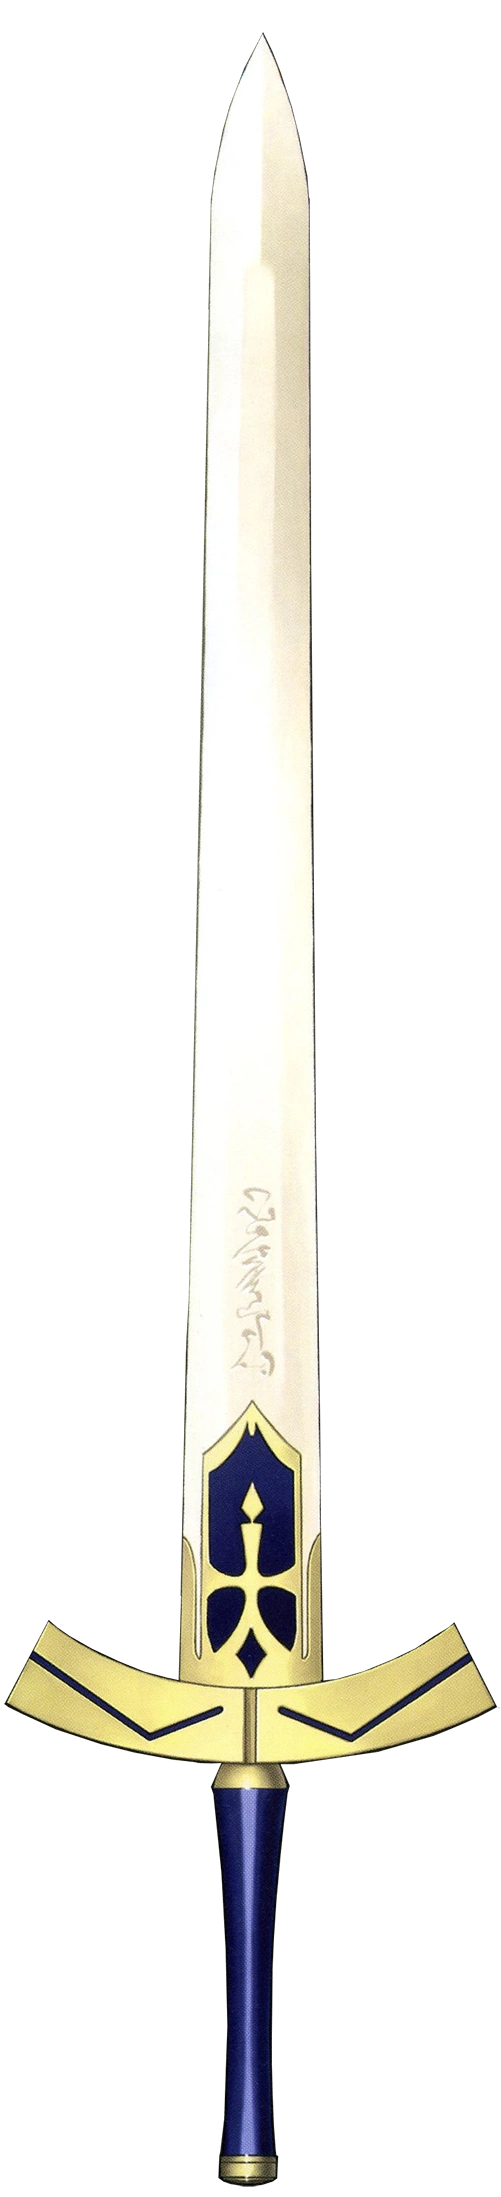
\includegraphics[width=0.15\textwidth]{Figs/Crests/Excalibur}}

%% College shield [optional] 
% Crest minimum should be 30mm.
%\collegeshield{\includegraphics[width=0.2\textwidth]{CollegeShields/Kings}}


%% Supervisor (optional)
%% for multiple supervisors, append each supervisor with the \newline command
%\supervisor{Prof. A.B. Supervisor\newline
%Prof. C.D. Supervisor}

%% Supervisor Role (optional) - Supervisor (default) or advisor
% \supervisorrole{\textbf{Supervisors: }}
%% if no title is desired:
% \supervisorrole{}

%% Supervisor line width: required to align supervisors
%\supervisorlinewidth{0.35\textwidth}

%% Advisor (optional)
%% for multiple advisors, append each advisor with the \newline command
%\advisor{Dr. A. Advisor\newline
%Dr. B. Advisor}
     
%% Advisor Role (optional) - Advisor (default) or leave empty
% \advisorrole{Advisors: }
%% if no title is required
% \advisorrole{}

%% Advisor line width: required to align supervisors
%\advisorlinewidth{0.25\textwidth}


%% You can redefine the submission text:
% Default as per the University guidelines:
% ``This dissertation is submitted for the degree of''
%\renewcommand{\submissiontext}{change the default text here if needed}

%% Full title of the Degree
\degreetitle{Doctor of Philosophy}

%% College affiliation (optional)
\college{Wolfson College}

%% Submission date
% Default is set as {\monthname[\the\month]\space\the\year}
%\degreedate{September 2014} 

%% Meta information
\subject{LaTeX} \keywords{{LaTeX} {PhD Thesis} {Physics} {University of
Cambridge}}


% ***************************** Abstract Separate ******************************
% To printout only the titlepage and the abstract with the PhD title and the
% author name for submission to the Student Registry, use the `abstract' option in
% the document class.

\ifdefineAbstract
 \pagestyle{empty}
 \includeonly{Declaration/declaration, Abstract/abstract}
\fi

% ***************************** Chapter Mode ***********************************
% The chapter mode allows user to only print particular chapters with references
% Title, Contents, Frontmatter are disabled by default
% Useful option to review a particular chapter or to send it to supervisior.
% To use choose `chapter' option in the document class

\ifdefineChapter
 \includeonly{Chapter3/chapter3}
\fi

% ******************************** Front Matter ********************************
\begin{document}

\frontmatter

\maketitle

\begin{crests}

\hspace{25mm}

\includegraphics[width=0.20\textwidth]{Figs/Crests/Family_Crest}
\newline

\vspace{60mm}

\includegraphics[width=0.20\textwidth]{Figs/Crests/University_Crest.pdf}
\hspace{70mm}

\includegraphics[width=36mm, height=38mm]{Figs/Crests/Wolfson_Crest.png}

\end{crests}
% ******************************* Thesis Dedidcation ********************************

\begin{dedication} 

I would like to dedicate this thesis to my loving parents \dots

\end{dedication}
% ******************************* Thesis Declaration ***************************

\begin{declaration}

This dissertation is the result of my own work and includes nothing which is the outcome of work done in collaboration except as declared in the Preface and specified in the text. It is not substantially the same as any work that has already been submitted, or, is being concurrently submitted for a degree, diploma or other qualification at the University of Cambridge, or any other university or similar institution except as declared in the Preface and specified in the text. It does not exceed the prescribed word limit for the Faculty of Physics \& Chemistry Degree Committee.

\Cref{sec:21cm} reviews decades of research in 21-cm cosmology following the work of many authors cited throughout. \Cref{sec:edges} summarises the work done in relation to the experiments published as \citet{edgesNature} with \cref{sec:historic_cal} detailing the calibration methods used in the EDGES experiment introduced by \citet{rogersCal} and \citet{edgesCal}, though some equations have been changed in this thesis to conform with modern notation. \Cref{sec:receiver_general}, \cref{sec:additional_models} and \cref{sec:matlab_results} are intended to be published as \mbox{\citet{nimaCal}} which was initially co-written with Dr. Nima Razavi-Ghods. The work presented in this thesis has been rewritten and expanded to incorporate details not included in \citet{nimaCal}. Computer aided design (CAD) models for various devices developed for these experiments were created by Steven H. Carey and are credited as such in the image descriptions. Some of the CAD images and files have been altered by the author for presentation in this thesis. The experiment regarding the front-end thermal management system effectiveness on six litres of water was done independently by Steven H. Carey but is included here for completeness. \Cref{sec:reach_formalism}, \cref{sec:likelihood} and \cref{sec:simulated_data} have been published as \citet{ian_bayes}. \Cref{sec:mphil_results} summarises work submitted to the University of Cambridge for an MPhil degree entitled ‘Bayesian Techniques for the Calibration of 21 cm Global Experiments’. \Cref{sec:fbf} is work intended to be published by the author at a later date. \Cref{fig:amp1_schematic}, \cref{fig:amp2_schematic} and \cref{fig:fem_schematic} are circuit diagrams created by John A. Ely based on designs by Dr. Nima Razavi-Ghods.


\end{declaration}

% ************************** Thesis Acknowledgements **************************

\begin{acknowledgements}      

Firstly, my deepest appreciation (and sincerest apologies) go to my two supervisors; Dr. Nima Razavi-Ghods and Dr. Will Handley for their continued support, guidance and patience. I know I could not have been the easiest person to work with, and I am eternally grateful to have been taken on as a student by them.

Thanks to my dearest parents Thomas and Solon; I can’t believe how lucky I am to be their son. I wouldn’t trade it for the world.

Thanks to my loving family; Andrew, Ben, Dick, Lily, Matthew, May, Rachel, Solia and Susie, for waiting so patiently for me, and to my cherished grandmothers, Camila and Betty, for their everlasting love.

I truly could not have done this without my darling Sabrina. My heartfelt gratitude for putting up with me dear. A very special thanks to Waldemar and Martina for opening up their home to me, especially during the most critical and difficult periods of thesis writing. And thanks to Martha for the endless support and affection.

I am honoured by the fellowship and assistance of Dr. William Barker. Appreciation goes to Dr. Florian Lienhard for being the best office mate anyone could ask for, and to Prof. Dave Green for being the best office neighbour anyone could ask for. I also wish to acknowledge Steve Carey and John Ely whose hard work and knowledge were integral to this project, for which I am truly grateful. I am very grateful to my group as well. Dr. Dominic Anstey generously provided much of his time and expertise teaching me the mathematical background of which this work is based. Dr. Harry Bevins provided an ideal to strive for. Dr. John Cumner listened to every single one of my rants and helped me pull through on my worst days. Thomas Gessey-Jones patiently and thoroughly answered all of my questions regardless of how trivial they were or how many times I walked into his office unannounced. Thanks goes to Sam Leeney for all the support and lunchtime chats. I also wish to thank Kilian Scheutwinkel for all of the advice and encouragement. It really meant a lot to me.

Thanks goes to Prof. Patrick Carrazana for believing in me, to Prof. Richard Saunders for his boundless wisdom and to Dr. Thomas Feggeler for the continued professional advice. I am truly grateful for the guidance of Dr. Christopher O’Grady, Dr. Monarin Uervirojnangkoorn and Prof. Stefano Profumo. I would not be here without them. For changing how I see the world, I would like to thank Prof. Richard Mitchell and for starting me on this journey, I would like to acknowledge Mr. Steve Ratto. Ms. Katherine (Katie) E. Ward showed me endless kindness for which I am honoured as well. I am indebted to so many wonderful teachers who taught, supported and encouraged me including; Prof. Steven Ritz, Prof. George Brown, Prof. Enrico Ramirez‑Ruiz, Dr. Adriane Steinacker, Mr. Arron Apperson, Mr. Nate Kundin, Mr. David Martin, Mr. Asif Rahman, Mr. Rich Serrao, and Mrs. Cristina Trujillo.

I am grateful to Dr. Anas Al Rawi, Prof. Paul Rimmer, Mr. Anthony Djedi and Mr. Steven Brereton for their pastoral and professional support and to all my treasured friends met along the way; Khalid Aleem, Morgan Dang, Joe Ferris, Khalen Hudson, Perman Jorayev, Edii Lam, Liam Lau, James Luis, Derek Ngoon, Michael O'Donnghaile, Peter Pedersen, and Matt Wang. Franklin, Derek and Arun were the most genuine of friends even when I wasn’t, and I could not have done any of this without Will Mandell.

I give thanks to John and Michelle Bentley for their sincere kindness and belief in me. I would also like to acknowledge the colleagues we’ve lost; Prof. Richard Hills and Dr. David Sun who challenge us to be the best of scientists and of course, my beloved auntie Solane.

And finally, thanks goes to those who inspired me to undertake this endeavour in the first place; Dr. Neil deGrasse Tyson, Prof. Brian Greene, Prof. Brian Cox and Prof. Michio Kaku.

\end{acknowledgements}

% ************************** Thesis Abstract *****************************
% Use `abstract' as an option in the document class to print only the titlepage and the abstract.
\begin{abstract}
The detection of minute radio-frequency signals from the primordial Universe are thought to contain fundamental information on the evolution of the first luminous sources. Such breakthroughs however are hindered by the unprecedented levels of sensitivity and calibration needed to confidently distinguish these millikelvin-level signatures from galactic foregrounds and instrument systematics. In this work we detail the development of a calibration methodology that expands upon the Dicke switching procedure introduced for microwave-frequency devices and applies it to contemporary experiments targeting early time periods such as the Dark Ages, Cosmic Dawn and Epoch of Reionisation.

Included are the designs and practical considerations for a receiver unit housing numerous calibration standards, a compact microcontroller unit, portable vector network analyser and Peltier-based thermal management system for deployment with the REACH radiometer experiment in the South African Radio Astronomy Observatory. Following this, we detail a first-of-its-kind Bayesian calibration algorithm named \textsc{Excalibrate} which offers unparalleled speed and mobility, allowing for the characterisation of the radiometer in the same environment as observational measurements. Datasets taken at various points of the receiver development are tested with \textsc{Excalibrate} which archives calibration accuracies of about 1 kelvin or less.

Upon numerous adjustments to both the physical receiver unit and our code, we demonstrate that the polynomial approximation for calibration parameters used by \textsc{Excalibrate} may not be an appropriate model for continued advancement towards a tens-of-millikelvin-level calibration accuracy. We believe this finding is corroborated by the EDGES team, which calls into question the controversal results reported by them using similar polynomial approximations. In light of this, we derive a mathematical framework for an alternative method to solve for calibration parameters as singular values at each frequency point and conclude with further suggestions for increasing the sensitivity of the radiometer.

\end{abstract}


% *********************** Adding TOC and List of Figures ***********************

\tableofcontents

\listoffigures

\listoftables

% \printnomenclature[space] space can be set as 2em between symbol and description
%\printnomenclature[3em]

\printnomenclature

% ******************************** Main Matter *********************************
\mainmatter

%!TEX root = ../thesis.tex
%*******************************************************************************
%*********************************** First Chapter *****************************
%*******************************************************************************
\pagenumbering{arabic}  

\chapter{Getting started}  %Title of the First Chapter

\ifpdf
    \graphicspath{{Chapter1/Figs/Raster/}{Chapter1/Figs/PDF/}{Chapter1/Figs/}}
\else
    \graphicspath{{Chapter1/Figs/Vector/}{Chapter1/Figs/}}
\fi


%********************************** %First Section  **************************************
\section{What is loren ipsum? Title with math \texorpdfstring{$\sigma$}{[sigma]}} %Section - 1.1 

Lorem Ipsum is simply dummy text of the printing and typesetting industry (see 
Section~\ref{section1.3}). Lorem Ipsum~\citep{Aup91} has been the industry's 
standard dummy text ever since the 1500s, when an unknown printer took a galley 
of type and scrambled it to make a type specimen book. It has survived not only 
five centuries, but also the leap into electronic typesetting, remaining 
essentially unchanged. It was popularised in the 1960s with the release of 
Letraset sheets containing Lorem Ipsum passages, and more recently with desktop 
publishing software like Aldus PageMaker including versions of Lorem 
Ipsum~\citep{AAB95,Con90,LM65}.

The most famous equation in the world: $E^2 = (m_0c^2)^2 + (pc)^2$, which is 
known as the \textbf{energy-mass-momentum} relation as an in-line equation.

A {\em \LaTeX{} class file}\index{\LaTeX{} class file@LaTeX class file} is a file, which holds style information for a particular \LaTeX{}.


\begin{align}
CIF: \hspace*{5mm}F_0^j(a) = \frac{1}{2\pi \iota} \oint_{\gamma} \frac{F_0^j(z)}{z - a} dz
\end{align}

\nomenclature[z-cif]{$CIF$}{Cauchy's Integral Formula}                                % first letter Z is for Acronyms 
\nomenclature[a-F]{$F$}{complex function}                                                   % first letter A is for Roman symbols
\nomenclature[g-p]{$\pi$}{ $\simeq 3.14\ldots$}                                             % first letter G is for Greek Symbols
\nomenclature[g-i]{$\iota$}{unit imaginary number $\sqrt{-1}$}                      % first letter G is for Greek Symbols
\nomenclature[g-g]{$\gamma$}{a simply closed curve on a complex plane}  % first letter G is for Greek Symbols
\nomenclature[x-i]{$\oint_\gamma$}{integration around a curve $\gamma$} % first letter X is for Other Symbols
\nomenclature[r-j]{$j$}{superscript index}                                                       % first letter R is for superscripts
\nomenclature[s-0]{$0$}{subscript index}                                                        % first letter S is for subscripts


%********************************** %Second Section  *************************************
\section{Why do we use loren ipsum?} %Section - 1.2


It is a long established fact that a reader will be distracted by the readable content of a page when looking at its layout. The point of using Lorem Ipsum is that it has a more-or-less normal distribution of letters, as opposed to using `Content here, content here', making it look like readable English. Many desktop publishing packages and web page editors now use Lorem Ipsum as their default model text, and a search for `lorem ipsum' will uncover many web sites still in their infancy. Various versions have evolved over the years, sometimes by accident, sometimes on purpose (injected humour and the like).

%********************************** % Third Section  *************************************
\section{Where does it come from?}  %Section - 1.3 
\label{section1.3}

Contrary to popular belief, Lorem Ipsum is not simply random text. It has roots in a piece of classical Latin literature from 45 BC, making it over 2000 years old. Richard McClintock, a Latin professor at Hampden-Sydney College in Virginia, looked up one of the more obscure Latin words, consectetur, from a Lorem Ipsum passage, and going through the cites of the word in classical literature, discovered the undoubtable source. Lorem Ipsum comes from sections 1.10.32 and 1.10.33 of "de Finibus Bonorum et Malorum" (The Extremes of Good and Evil) by Cicero, written in 45 BC. This book is a treatise on the theory of ethics, very popular during the Renaissance. The first line of Lorem Ipsum, "Lorem ipsum dolor sit amet..", comes from a line in section 1.10.32.

The standard chunk of Lorem Ipsum used since the 1500s is reproduced below for those interested. Sections 1.10.32 and 1.10.33 from ``de Finibus Bonorum et Malorum" by Cicero are also reproduced in their exact original form, accompanied by English versions from the 1914 translation by H. Rackham

``Lorem ipsum dolor sit amet, consectetur adipisicing elit, sed do eiusmod tempor incididunt ut labore et dolore magna aliqua. Ut enim ad minim veniam, quis nostrud exercitation ullamco laboris nisi ut aliquip ex ea commodo consequat. Duis aute irure dolor in reprehenderit in voluptate velit esse cillum dolore eu fugiat nulla pariatur. Excepteur sint occaecat cupidatat non proident, sunt in culpa qui officia deserunt mollit anim id est laborum."

Section 1.10.32 of ``de Finibus Bonorum et Malorum", written by Cicero in 45 BC: ``Sed ut perspiciatis unde omnis iste natus error sit voluptatem accusantium doloremque laudantium, totam rem aperiam, eaque ipsa quae ab illo inventore veritatis et quasi architecto beatae vitae dicta sunt explicabo. Nemo enim ipsam voluptatem quia voluptas sit aspernatur aut odit aut fugit, sed quia consequuntur magni dolores eos qui ratione voluptatem sequi nesciunt. Neque porro quisquam est, qui dolorem ipsum quia dolor sit amet, consectetur, adipisci velit, sed quia non numquam eius modi tempora incidunt ut labore et dolore magnam aliquam quaerat voluptatem. Ut enim ad minima veniam, quis nostrum exercitationem ullam corporis suscipit laboriosam, nisi ut aliquid ex ea commodi consequatur? Quis autem vel eum iure reprehenderit qui in ea voluptate velit esse quam nihil molestiae consequatur, vel illum qui dolorem eum fugiat quo voluptas nulla pariatur?"

1914 translation by H. Rackham: ``But I must explain to you how all this mistaken idea of denouncing pleasure and praising pain was born and I will give you a complete account of the system, and expound the actual teachings of the great explorer of the truth, the master-builder of human happiness. No one rejects, dislikes, or avoids pleasure itself, because it is pleasure, but because those who do not know how to pursue pleasure rationally encounter consequences that are extremely painful. Nor again is there anyone who loves or pursues or desires to obtain pain of itself, because it is pain, but because occasionally circumstances occur in which toil and pain can procure him some great pleasure. To take a trivial example, which of us ever undertakes laborious physical exercise, except to obtain some advantage from it? But who has any right to find fault with a man who chooses to enjoy a pleasure that has no annoying consequences, or one who avoids a pain that produces no resultant pleasure?"

Section 1.10.33 of ``de Finibus Bonorum et Malorum", written by Cicero in 45 BC: ``At vero eos et accusamus et iusto odio dignissimos ducimus qui blanditiis praesentium voluptatum deleniti atque corrupti quos dolores et quas molestias excepturi sint occaecati cupiditate non provident, similique sunt in culpa qui officia deserunt mollitia animi, id est laborum et dolorum fuga. Et harum quidem rerum facilis est et expedita distinctio. Nam libero tempore, cum soluta nobis est eligendi optio cumque nihil impedit quo minus id quod maxime placeat facere possimus, omnis voluptas assumenda est, omnis dolor repellendus. Temporibus autem quibusdam et aut officiis debitis aut rerum necessitatibus saepe eveniet ut et voluptates repudiandae sint et molestiae non recusandae. Itaque earum rerum hic tenetur a sapiente delectus, ut aut reiciendis voluptatibus maiores alias consequatur aut perferendis doloribus asperiores repellat."

1914 translation by H. Rackham: ``On the other hand, we denounce with righteous indignation and dislike men who are so beguiled and demoralized by the charms of pleasure of the moment, so blinded by desire, that they cannot foresee the pain and trouble that are bound to ensue; and equal blame belongs to those who fail in their duty through weakness of will, which is the same as saying through shrinking from toil and pain. These cases are perfectly simple and easy to distinguish. In a free hour, when our power of choice is untrammelled and when nothing prevents our being able to do what we like best, every pleasure is to be welcomed and every pain avoided. But in certain circumstances and owing to the claims of duty or the obligations of business it will frequently occur that pleasures have to be repudiated and annoyances accepted. The wise man therefore always holds in these matters to this principle of selection: he rejects pleasures to secure other greater pleasures, or else he endures pains to avoid worse pains."

\nomenclature[z-DEM]{DEM}{Discrete Element Method}
\nomenclature[z-FEM]{FEM}{Finite Element Method}
\nomenclature[z-PFEM]{PFEM}{Particle Finite Element Method}
\nomenclature[z-FVM]{FVM}{Finite Volume Method}
\nomenclature[z-BEM]{BEM}{Boundary Element Method}
\nomenclature[z-MPM]{MPM}{Material Point Method}
\nomenclature[z-LBM]{LBM}{Lattice Boltzmann Method}
\nomenclature[z-MRT]{MRT}{Multi-Relaxation 
Time}
\nomenclature[z-RVE]{RVE}{Representative Elemental Volume}
\nomenclature[z-GPU]{GPU}{Graphics Processing Unit}
\nomenclature[z-SH]{SH}{Savage Hutter}
\nomenclature[z-CFD]{CFD}{Computational Fluid Dynamics}
\nomenclature[z-LES]{LES}{Large Eddy Simulation}
\nomenclature[z-FLOP]{FLOP}{Floating Point Operations}
\nomenclature[z-ALU]{ALU}{Arithmetic Logic Unit}
\nomenclature[z-FPU]{FPU}{Floating Point Unit}
\nomenclature[z-SM]{SM}{Streaming Multiprocessors}
\nomenclature[z-PCI]{PCI}{Peripheral Component Interconnect}
\nomenclature[z-CK]{CK}{Carman - Kozeny}
\nomenclature[z-CD]{CD}{Contact Dynamics}
\nomenclature[z-DNS]{DNS}{Direct Numerical Simulation}
\nomenclature[z-EFG]{EFG}{Element-Free Galerkin}
\nomenclature[z-PIC]{PIC}{Particle-in-cell}
\nomenclature[z-USF]{USF}{Update Stress First}
\nomenclature[z-USL]{USL}{Update Stress Last}
\nomenclature[s-crit]{crit}{Critical state}
\nomenclature[z-DKT]{DKT}{Draft Kiss Tumble}
\nomenclature[z-PPC]{PPC}{Particles per cell}
%!TEX root = ../thesis.tex
%*******************************************************************************
%****************************** Second Chapter *********************************
%*******************************************************************************

\chapter{My second chapter}

\ifpdf
    \graphicspath{{Chapter2/Figs/Raster/}{Chapter2/Figs/PDF/}{Chapter2/Figs/}}
\else
    \graphicspath{{Chapter2/Figs/Vector/}{Chapter2/Figs/}}
\fi


\section[Short title]{Reasonably long section title}

% Uncomment this line, when you have siunitx package loaded.
%The SI Units for dynamic viscosity is \si{\newton\second\per\metre\squared}.
I'm going to randomly include a picture Figure~\ref{fig:minion}.


If you have trouble viewing this document contact Krishna at: \href{mailto:kks32@cam.ac.uk}{kks32@cam.ac.uk} or raise an issue at \url{https://github.com/kks32/phd-thesis-template/}


\begin{figure}[htbp!] 
\centering    

\includegraphics[width=1.0\textwidth]{minion}
\caption[Minion]{This is just a long figure caption for the minion in Despicable Me from Pixar}
\label{fig:minion}
\end{figure}


\section*{Enumeration}
Lorem ipsum dolor sit amet, consectetur adipiscing elit. Sed vitae laoreet lectus. Donec lacus quam, malesuada ut erat vel, consectetur eleifend tellus. Aliquam non feugiat lacus. Interdum et malesuada fames ac ante ipsum primis in faucibus. Quisque a dolor sit amet dui malesuada malesuada id ac metus. Phasellus posuere egestas mauris, sed porta arcu vulputate ut. Donec arcu erat, ultrices et nisl ut, ultricies facilisis urna. Quisque iaculis, lorem non maximus pretium, dui eros auctor quam, sed sodales libero felis vel orci. Aliquam neque nunc, elementum id accumsan eu, varius eu enim. Aliquam blandit ante et ligula tempor pharetra. Donec molestie porttitor commodo. Integer rutrum turpis ac erat tristique cursus. Sed venenatis urna vel tempus venenatis. Nam eu rhoncus eros, et condimentum elit. Quisque risus turpis, aliquam eget euismod id, gravida in odio. Nunc elementum nibh risus, ut faucibus mauris molestie eu.
 Vivamus quis nunc nec nisl vulputate fringilla. Duis tempus libero ac justo laoreet tincidunt. Fusce sagittis gravida magna, pharetra venenatis mauris semper at. Nullam eleifend felis a elementum sagittis. In vel turpis eu metus euismod tempus eget sit amet tortor. Donec eu rhoncus libero, quis iaculis lectus. Aliquam erat volutpat. Proin id ullamcorper tortor. Fusce vestibulum a enim non volutpat. Nam ut interdum nulla. Proin lacinia felis malesuada arcu aliquet fringilla. Aliquam condimentum, tellus eget maximus porttitor, quam sem luctus massa, eu fermentum arcu diam ac massa. Praesent ut quam id leo molestie rhoncus. Praesent nec odio eget turpis bibendum eleifend non sit amet mi. Curabitur placerat finibus velit, eu ultricies risus imperdiet ut. Suspendisse lorem orci, luctus porta eros a, commodo maximus nisi.

Nunc et dolor diam. Phasellus eu justo vitae diam vehicula tristique. Vestibulum vulputate cursus turpis nec commodo. Etiam elementum sit amet erat et pellentesque. In eu augue sed tortor mollis tincidunt. Mauris eros dui, sagittis vestibulum vestibulum vitae, molestie a velit. Donec non felis ut velit aliquam convallis sit amet sit amet velit. Aliquam vulputate, elit in lacinia lacinia, odio lacus consectetur quam, sit amet facilisis mi justo id magna. Curabitur aliquet pulvinar eros. Cras metus enim, tristique ut magna a, interdum egestas nibh. Aenean lorem odio, varius a sollicitudin non, cursus a odio. Vestibulum ante ipsum primis in faucibus orci luctus et ultrices posuere cubilia Curae; 
\begin{enumerate}
\item The first topic is dull
\item The second topic is duller
\begin{enumerate}
\item The first subtopic is silly
\item The second subtopic is stupid
\end{enumerate}
\item The third topic is the dullest
\end{enumerate}
Morbi bibendum est aliquam, hendrerit dolor ac, pretium sem. Nunc molestie, dui in euismod finibus, nunc enim viverra enim, eu mattis mi metus id libero. Cras sed accumsan justo, ut volutpat ipsum. Nam faucibus auctor molestie. Morbi sit amet eros a justo pretium aliquet. Maecenas tempor risus sit amet tincidunt tincidunt. Curabitur dapibus gravida gravida. Vivamus porta ullamcorper nisi eu molestie. Ut pretium nisl eu facilisis tempor. Nulla rutrum tincidunt justo, id placerat lacus laoreet et. Sed cursus lobortis vehicula. Donec sed tortor et est cursus pellentesque sit amet sed velit. Proin efficitur posuere felis, porta auctor nunc. Etiam non porta risus. Pellentesque lacinia eros at ante iaculis, sed aliquet ipsum volutpat. Suspendisse potenti.

Ut ultrices lectus sed sagittis varius. Nulla facilisi. Nullam tortor sem, placerat nec condimentum eu, tristique eget ex. Nullam pretium tellus ut nibh accumsan elementum. Aliquam posuere gravida tellus, id imperdiet nulla rutrum imperdiet. Nulla pretium ullamcorper quam, non iaculis orci consectetur eget. Curabitur non laoreet nisl. Maecenas lacinia, lorem vel tincidunt cursus, odio lorem aliquet est, gravida auctor arcu urna id enim. Morbi accumsan bibendum ipsum, ut maximus dui placerat vitae. Nullam pretium ac tortor nec venenatis. Nunc non aliquet neque. 

\section*{Itemize}
\begin{itemize}
\item The first topic is dull
\item The second topic is duller
\begin{itemize}
\item The first subtopic is silly
\item The second subtopic is stupid
\end{itemize}
\item The third topic is the dullest
\end{itemize}

\section*{Description}
\begin{description}
\item[The first topic] is dull
\item[The second topic] is duller
\begin{description}
\item[The first subtopic] is silly
\item[The second subtopic] is stupid
\end{description}
\item[The third topic] is the dullest
\end{description}


\clearpage

\tochide\section{Hidden section}
\textbf{Lorem ipsum dolor sit amet}, \textit{consectetur adipiscing elit}. In magna nisi, aliquam id blandit id, congue ac est. Fusce porta consequat leo. Proin feugiat at felis vel consectetur. Ut tempus ipsum sit amet congue posuere. Nulla varius rutrum quam. Donec sed purus luctus, faucibus velit id, ultrices sapien. Cras diam purus, tincidunt eget tristique ut, egestas quis nulla. Curabitur vel iaculis lectus. Nunc nulla urna, ultrices et eleifend in, accumsan ut erat. In ut ante leo. Aenean a lacinia nisl, sit amet ullamcorper dolor. Maecenas blandit, tortor ut scelerisque congue, velit diam volutpat metus, sed vestibulum eros justo ut nulla. Etiam nec ipsum non enim luctus porta in in massa. Cras arcu urna, malesuada ut tellus ut, pellentesque mollis risus.Morbi vel tortor imperdiet arcu auctor mattis sit amet eu nisi. Nulla gravida urna vel nisl egestas varius. Aliquam posuere ante quis malesuada dignissim. Mauris ultrices tristique eros, a dignissim nisl iaculis nec. Praesent dapibus tincidunt mauris nec tempor. Curabitur et consequat nisi. Quisque viverra egestas risus, ut sodales enim blandit at. Mauris quis odio nulla. Cras euismod turpis magna, in facilisis diam congue non. Mauris faucibus nisl a orci dictum, et tempus mi cursus.

Etiam elementum tristique lacus, sit amet eleifend nibh eleifend sed \footnote{My footnote goes blah blah blah! \dots}. Maecenas dapibu augue ut urna malesuada, non tempor nibh mollis. Donec sed sem sollicitudin, convallis velit aliquam, tincidunt diam. In eu venenatis lorem. Aliquam non augue porttitor tellus faucibus porta et nec ante. Proin sodales, libero vitae commodo sodales, dolor nisi cursus magna, non tincidunt ipsum nibh eget purus. Nam rutrum tincidunt arcu, tincidunt vulputate mi sagittis id. Proin et nisi nec orci tincidunt auctor et porta elit. Praesent eu dolor ac magna cursus euismod. Integer non dictum nunc.


\begin{landscape}

\section*{Subplots}
I can cite Wall-E (see Fig.~\ref{fig:WallE}) and Minions in despicable me (Fig.~\ref{fig:Minnion}) or I can cite the whole figure as Fig.~\ref{fig:animations}


\begin{figure}
  \centering
  \begin{subfigure}[b]{0.3\textwidth}
    
\includegraphics[width=\textwidth]{TomandJerry}
    \caption{Tom and Jerry}
    \label{fig:TomJerry}   
  \end{subfigure}             
  \begin{subfigure}[b]{0.3\textwidth}
    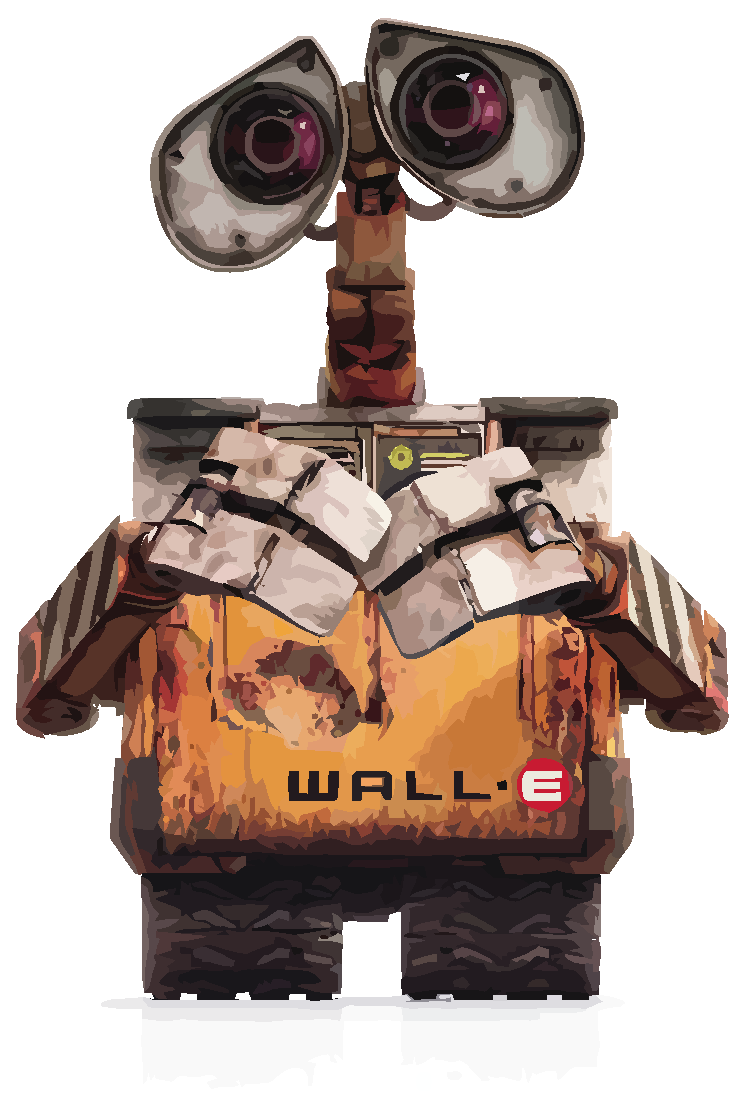
\includegraphics[width=\textwidth]{WallE}
    \caption{Wall-E}
    \label{fig:WallE}
  \end{subfigure}             
  \begin{subfigure}[b]{0.3\textwidth}
    
\includegraphics[width=\textwidth]{minion}
    \caption{Minions}
    \label{fig:Minnion}
  \end{subfigure}
  \caption{Best Animations}
  \label{fig:animations}
\end{figure}


\end{landscape}

\chapter{Receiver design and development}

% **************************** Define Graphics Path **************************
\ifpdf
    \graphicspath{{Chapter3/Figs/Raster/}{Chapter3/Figs/PDF/}{Chapter3/Figs/}}
\else
    \graphicspath{{Chapter3/Figs/Vector/}{Chapter3/Figs/}}
\fi

Measurements of the radio-sky require an instrument called a ‘radiometer’, a machine that measures incoming radiation. A radiometer usually consists of two main components; an antenna to collect an electromagnetic waves and a device to measure the signal's power such as a spectrometer. As more advanced instruments are deployed, additional processes are implemented to condition this information before being sent to the spectrometer such as amplification of weak signals and filtering to an frequencies of interest such that a new intermediary device is often introduced as a bridge between the antenna and the spectrometer known as a ‘receiver’.

The addition of components such as a receiver will necessarily produce more complicated forms of systematic noise, through things like reflections spawned from impedance mismatches at connections which hamper the detection and analysis of astrophysical phenomena. Characterising the interaction of the various instrument components as well as the resulting noise is undertaken through auxiliary devices which inform the process of ‘calibration’ in order to ultimately remove systematics and facilitate detection of cosmic signals. Consideration for the ensemble of devices, their control and monitoring is a principle area of experimental instrument design and the development of new architecture and engineering techniques to accommodate the unique requirements of individual experiments is the focus of this next chapter.


% =========================================
\section{The REACH receiver}
The REACH receiver is designed to address concerns brought forth with other experiments regarding residual systematics in their data while permitting the innovative features of the overall radiometer. Primarily, the broad bandwidth used by REACH makes it impractical to develop an achromatic antenna that provides a perfect impedance match between the antenna and receiver. Reflections spawned from this contact point result in considerable spectral variation across the observational band on the order of tens of Kelvin due to the overwhelming synchrotron foreground at these frequencies. Furthermore, while the method of ‘relative calibration’ was historically used to characterise narrow-band instruments, wide-band radiometers must obtain an absolute flux scale in frequency to measure the frequency-dependent sky-averaged brightness temperature through ‘absolute calibration’, which necessitates a series of additional components and switches.

Another primary focus of the design approach was the ability to calibrate the instrument completely in the field\footnote{While this philosophy was not completely adhered to in the final deployed system, the spirit of this ambition guided the entire receiver development. Please see CHAPTER ON S-PARAMETER CORRECTIONS for more details.} as opposed to previous experiments where the devices were characterised in controlled laboratory settings before deployment. The environmental (e.g. temperature and humidity) dependence of the sensitive electronic components provided a challenge to be addressed in the receiver design which requires system and temperature stability in the field as well as full autonomy.

In response to these considerations, the REACH receiver system is comprised of two subsystems, the receiver ‘front-end’ that sits under the raised antenna ground plane and the receiver ‘back-end’, also known as the readout system, which is separated from the front-end by a 100 metre distance connected by a Radio Frequency over Fibre (RFoF) link and powered by solar panels. A conceptual diagram of the radiometer system is shown in \cref{fig:system_diagram}. Many of the environment-sensitive components responsible for calibration and conditioning of the data are included in the front-end, with the back-end containing components for spectral data collection, control and signal processing as detailed below.
\begin{figure}
    \centering
    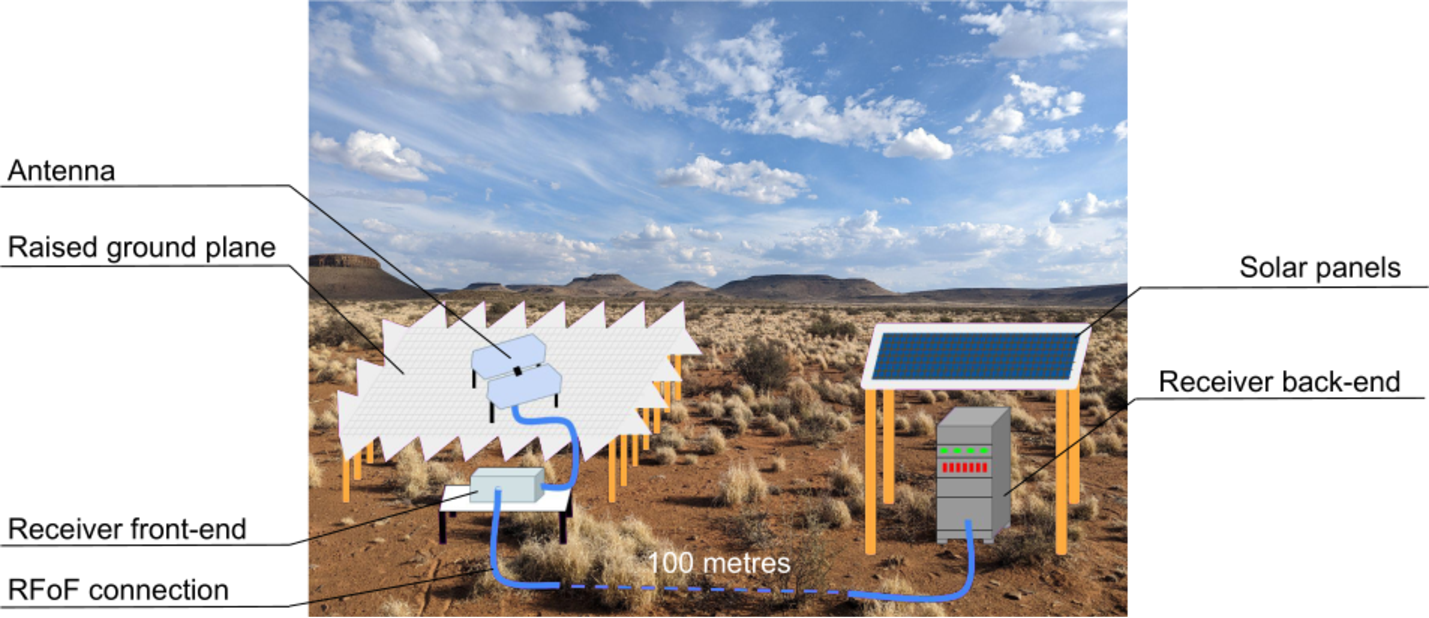
\includegraphics[width=\textwidth]{system_diagram}
    \caption{An illustration of the REACH radiometric system showing the hexagonal dipole antenna on a raised ground plane above the receiver front-end linked to the back-end and solar panels by 100 metres of fibre optic cable. The background image is a picture taken of the REACH deployment site located in the South African Karoo Radio Astronomy Reserve.}
    \label{fig:system_diagram}
\end{figure}


% =========================================
\subsection{Receiver front-end}
The front-end contains the most sensitive radiometer components housed in a sealed enclosure to facilitate calibration of the instrument to the highest accuracy. As the maintenance of environmental stability is difficult to achieve over long periods of time in the field, the project’s emphasis on an in situ calibration could only be achieved through a conscious effort to minimise the volume of the receiver front-end such that a constant temperature is kept via thermal devices while drawing a sustainable amount of power from the solar panels which are rated to give a maximum of 135 W of power to the front-end. Given this as a primary focus during the design process, nearly all of the components in the front-end were chosen based on a careful balance between their compact size and superior quality.


% =========================================
\subsubsection{The front-end enclosure}
The entirety of the receiver front-end is contained in a $500 \times 500 \times 210$ mm Rittal AE 1007.600 stainless steel enclosure serving as an RF-shield with category IP 66 protection against dust and water from the outside environment. 20 mm\footnote{18 mm in actuality when measured} of Kingspan Kooltherm K5 External Wall Insulation Board lines the inner walls of the enclosure in order to assist with temperature stability. Original designs used 11 mm Zotefoam for its efficient absorption of infrared radiation as used by the BICEP and Keck Array, but thermal tests showed this material to be less efficient during cooling compared to the 0.021 Wm\textsuperscript{-1}K\textsuperscript{-1} thermal conductivity of the building-standard Kooltherm sheets. Six connection ports were drilled into the enclosure to interface with external components; one for connection to the antenna sitting directly above the receiver on the raised ground plane via 150 mm Heliax cable, two for control and monitoring via USB over fibre-optical link, one RFoF connection for communication with the receiver back-end, one SubMiniature version-A (SMA) port for the 48 V DC power supply from the solar panels and an additional coaxial SMA port for testing and triage in the field. EMI gaskets were placed around the openings to reduce the impact of self-generated RFI towards the antenna as well as external RFI from feeding into the signal chain. A diagram of the enclosure’s external connections is shown in \cref{fig:enclosure_external_connections}.
\begin{figure}
    \centering
    \includegraphics[width=\textwidth]{enclosure_external_connections}
    \caption{The external connections of the receiver front-end enclosure showing the coaxial antenna connections, USB to fibre connections in blue, RFoF connection in green, power connection and additional port for in-field diagnostics and testing. The orientation shown is the same as during deployment.}
\label{fig:enclosure_external_connections}
\end{figure}

The metal framing of the enclosure also served as a heat dump for the encased electrical components using a custom heat exchanger and fan-assisted heat sink as detailed in the next section. To assist with the thermal considerations, the receiver front-end components are mounted on a 3 mm baseplate as shown in \cref{fig:enclosure_plate} to allow airflow between the plate and the internal heat exchanger.
\begin{figure}
    \centering
    \begin{minipage}{.4\textwidth}
        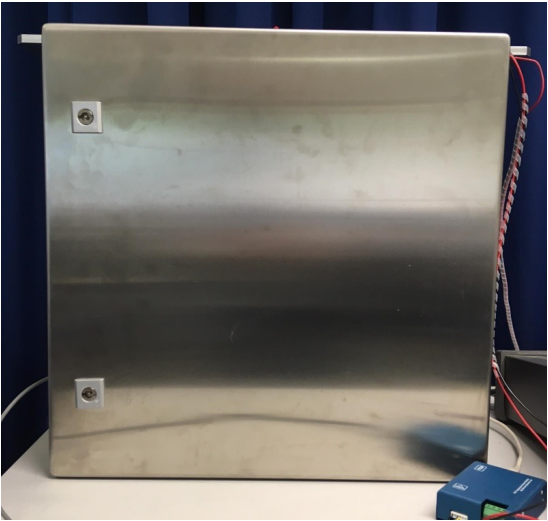
\includegraphics[scale=0.55]{enclosure}
        \vfill
        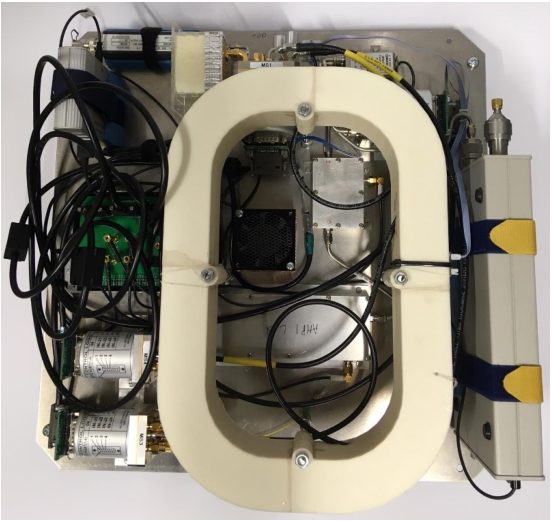
\includegraphics[scale=0.55]{component_plate}
    \end{minipage}
    \begin{minipage}{.4\textwidth}
        \centering
        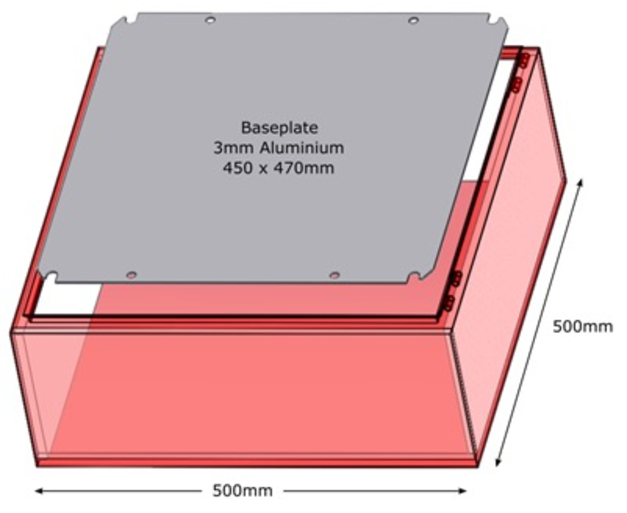
\includegraphics[scale=0.57]{enclosure_plate}
    \end{minipage}
    \caption{A picture of the front-end enclosure is shown on the top left. The bottom left shows the front-end components bolted onto the 3 mm baseplate. The diagram on the right depicts the baseplate's insertion into the enclosure.}
    \label{fig:enclosure_plate}
\end{figure}


% =========================================
\subsubsection{Front-end thermal management system}
Front-end temperature stability is maintained through a stack of components placed below the centre of the baseplate. A 113 watt Laird UltraTEC UT6-24-F1-5555 proportional integral derivative thermoelectric cooler (TEC) drives cooling or heating through the Peltier effect which is coupled to the receiver component baseplate by a $55 \times 55 \times 16$ mm copper stack. A thermal gap pad connects the bottom of the TEC module with a larger copper plate on the enclosure wall allowing heat transfer to an external Fischer LA7 150-1 heatsink and fan for expulsion of heat to the outside environment.

An initial test of this setup was conducted by placing a 40 W $110 \times 110$ mm heating source below the receiver component baseplate centre which recorded a 5 K (or 8 K?) temperature gradient over the plate as shown in \cref{fig:base_temp_grad}.
\begin{figure}
    \centering
    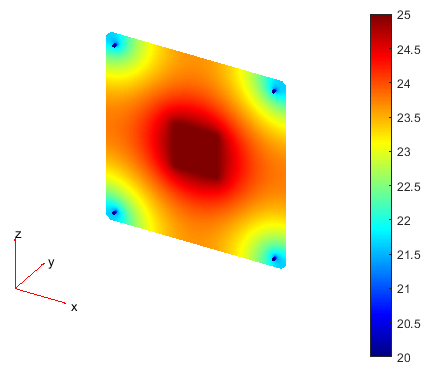
\includegraphics[scale=0.6]{base_temp_grad}
    \caption{A plot from an initial temperature test showing a 5 K temperature gradient over the receiver component baseplate when heated from below by a 40 W heat source placed at the plate's centre.}
    \label{fig:base_temp_grad}
\end{figure}
Following the results of this test, a secondary baseplate was installed below the initial baseplate with the two plates separated by a heatsink and an internal fan installed to promote air circulation throughout the front end. A follow-up test using this configuration returned a temperature gradient of 0.125 K across the component baseplate. A diagram of the completed setup is shown in \cref{fig:peltier_diag}
\begin{figure}
    \centering
    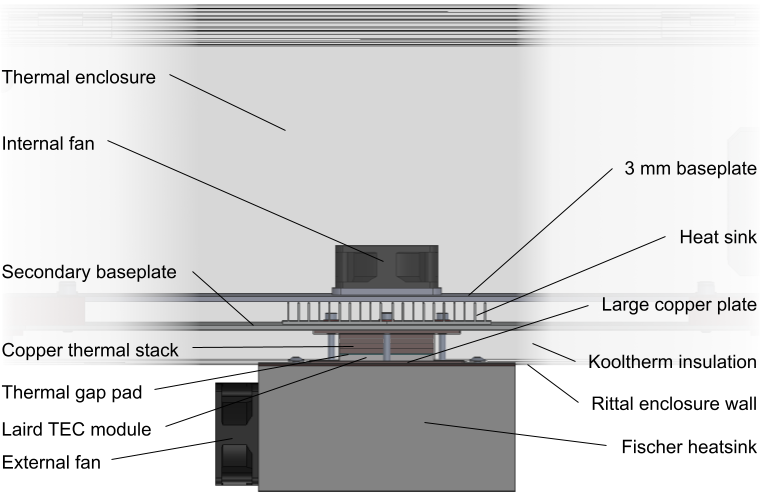
\includegraphics[width=\textwidth]{reach_peltier_diagram}
    \caption{A diagram representing the components for thermal conditioning of the receiver front-end. The vantage point shown is as if the front-end enclosure is laid on its back. It should be noted that the above figure is the MK II version which is slightly updated from the configuration currently deployed in the field.}
    \label{fig:peltier_diag}
\end{figure}

The TEC is controlled by an Electron Dynamics Southampton TC-M-U-10A module and powered by a separate custom-made 22 V power supply unit (PSU) designed to reduce RFI coupling from the very large switch currents produced. The PSU, shown in \cref{fig:psu}, is also configured to automatically power the external fan when the Electron Dynamics controller draws more than 6 W of power to prevent thermal overload.
\begin{figure}
    \centering
    \begin{subfigure}{.45\textwidth}
        \centering
        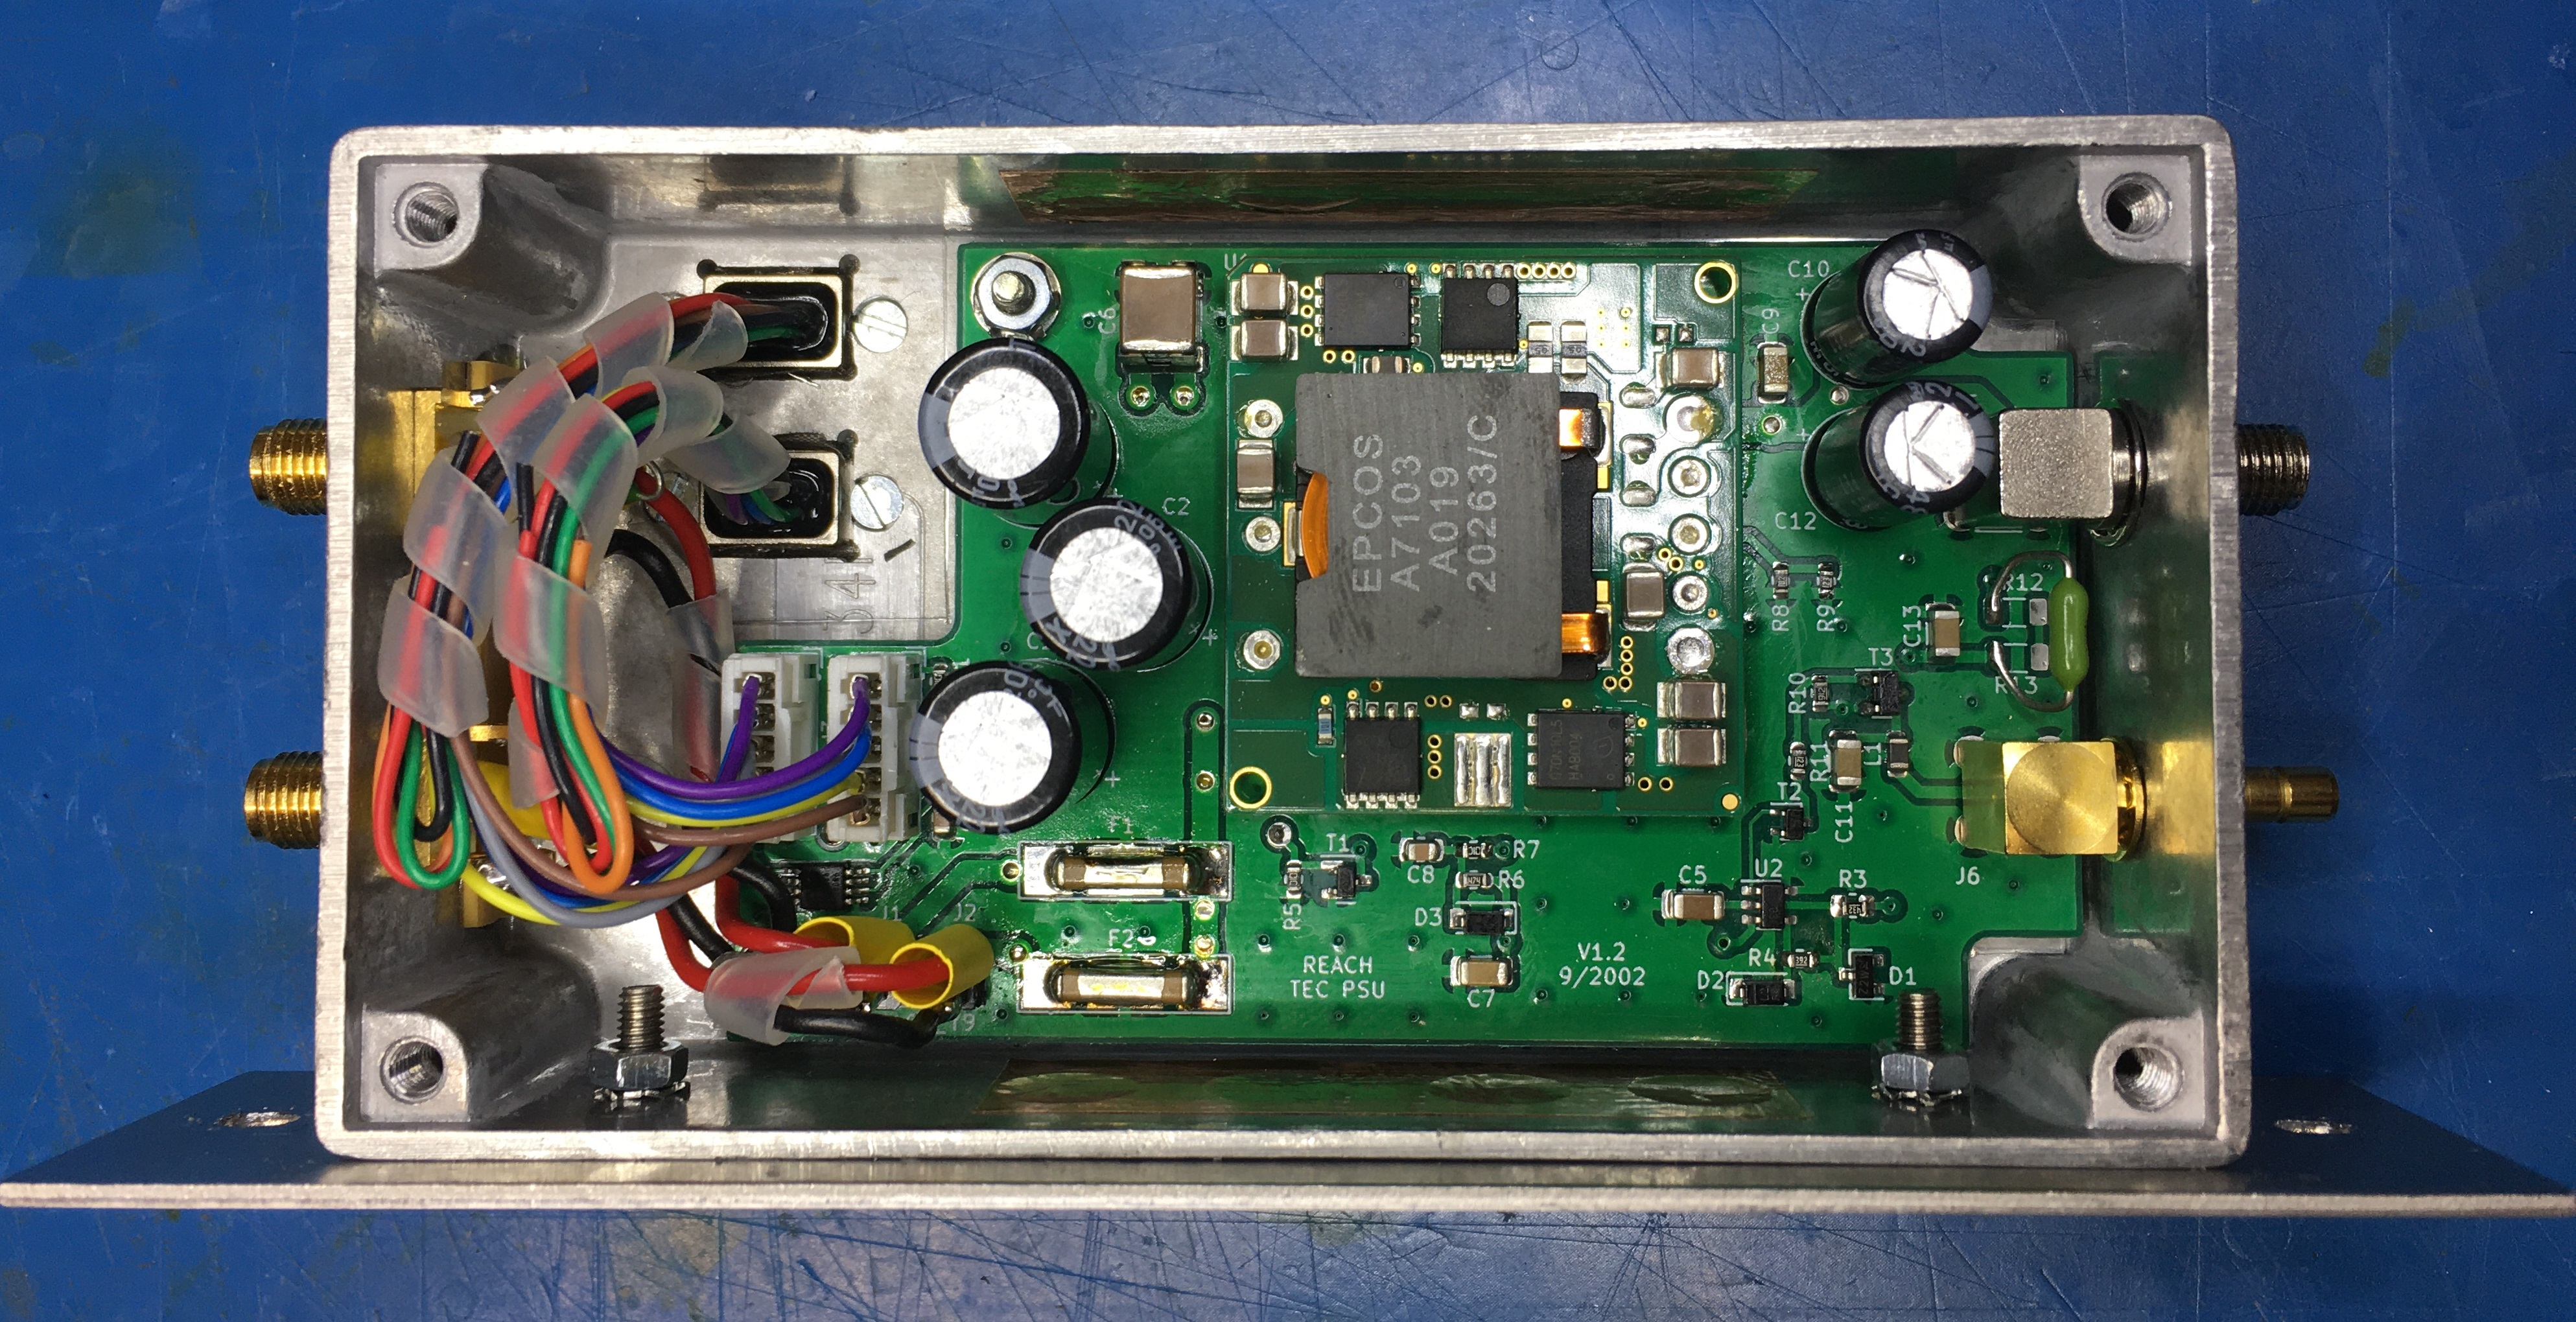
\includegraphics[width=\linewidth]{psu}
    \end{subfigure}
    \hfill
    \begin{subfigure}{.52\textwidth}
    \centering
        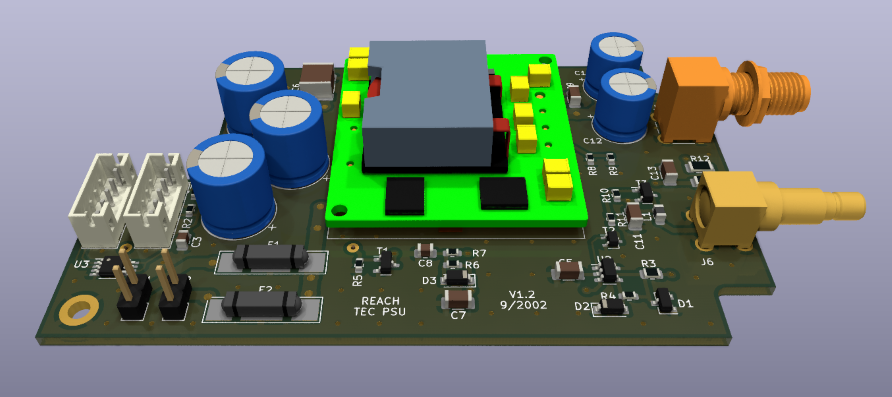
\includegraphics[width=\linewidth]{cad_psu}
    \end{subfigure}
    \caption{The constructed thermoelectric cooler power supply unit (left) along with its original CAD rendering (right) for perspective.}
    \label{fig:psu}
\end{figure}

The effectiveness of the front-end thermal management system was evaluated by testing the performance of the construction on 6 litres of bottled water placed in the empty front-end enclosure at room temperature with the TEC driven at its maximum 88 W and the Electron Dynamics controller instructed to maintain a $10^\circ$ C setpoint temperature as shown in \cref{fig:water_test} where the endpoint is achieved after about 8 hours of cooling with a steady-state temperature within 0.01 K of the target setpoint. These results suggest that a long, continuous amount of cooling is needed to stabilise the front-end temperature before calibration or observational measurements are made. This may be done in the afternoon or evenings preceding an observational run. OR FIND PLOT WITH TIME TAKES TO BRING FINALISED CONSTRUCTION TO SET POINT. An additional comparison of the completed thermal management system installed on the front-end enclosure with its 3D-rendered cross section is shown in \cref{fig:enclose_supp} for reference.
\begin{figure}
    \centering
    \centering
    \begin{subfigure}{.4\textwidth}
        \centering
        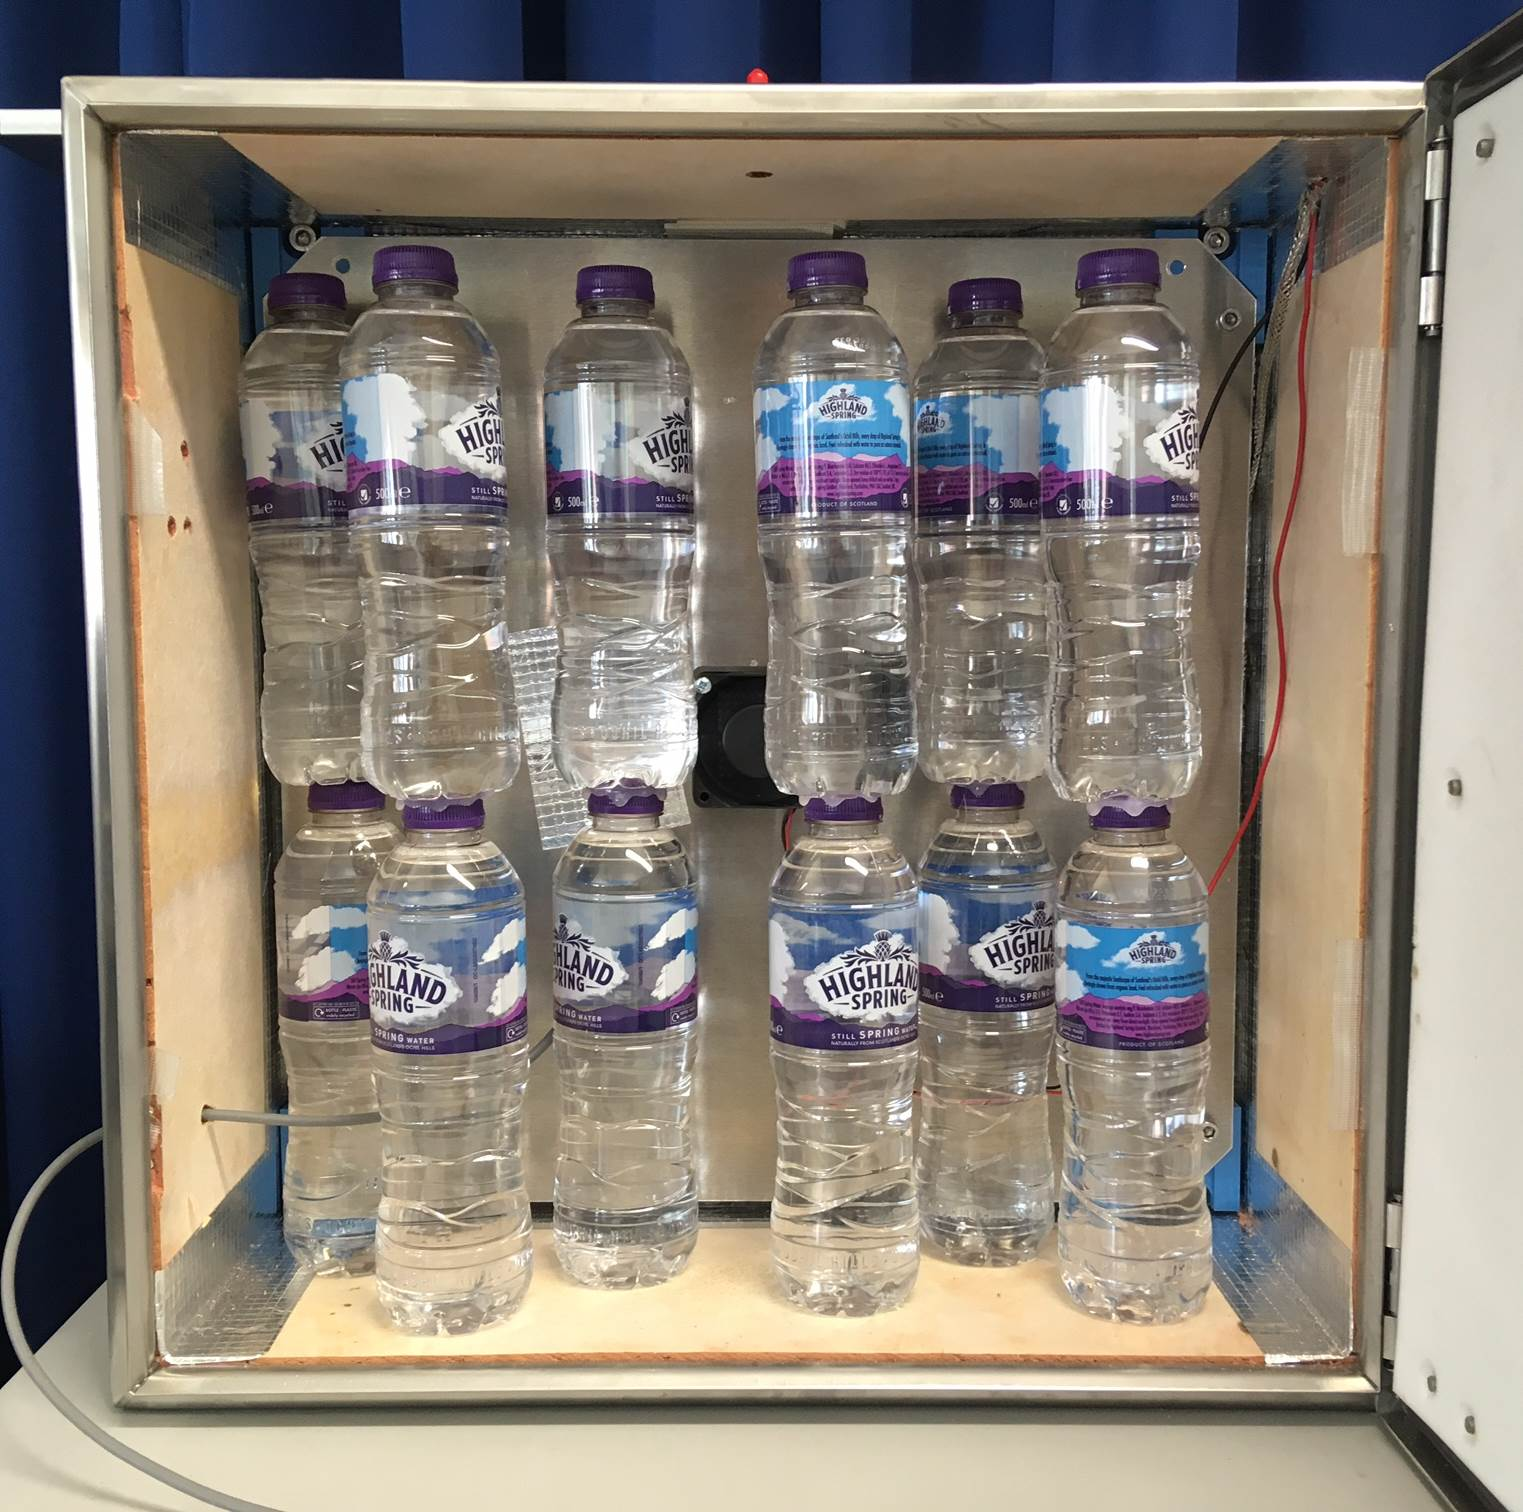
\includegraphics[width=\linewidth]{water}
    \end{subfigure}
    \hfill
    \begin{subfigure}{.55\textwidth}
    \centering
        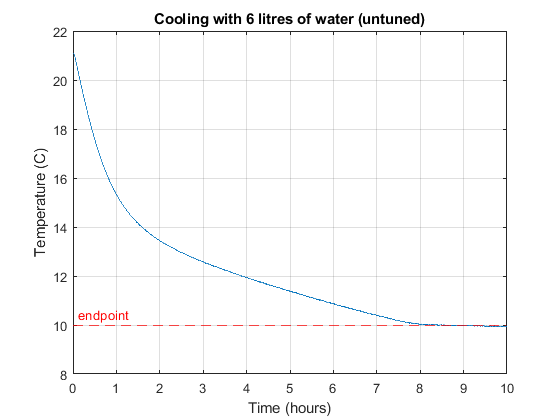
\includegraphics[width=\linewidth]{water_results}
    \end{subfigure}
    \caption{Six litres of water placed in the empty front-end enclosure with the thermal management system installed. The results of this test with the TEC driven at its maximum wattage and the controller setpoint of $10^\circ$ C is shown on the right. It should be noted that for this test, the proportional, integral and derivative controller values were not tuned beforehand, which reduces efficiency.}
    \label{fig:water_test}
\end{figure}


% =========================================
\subsubsection{Calibration sources}
One of the main obligations for thermal stability was to stabilise measurements of passive devices used to calibrate the instrument which we collectively refer to as ‘calibration sources’ or ‘calibrators’. Historically, absolute calibration is undertaken through measurement of each calibration source as part of a three-position Dicke cycle containing a single source, a reference $50 \Omega$ load and a reference noise source where comparison of power spectral measurements between the source and references serve to calibrate out time dependent system gain as detailed in REFERENCE Q-TERM EQUATION. Usually four sources were used; an ambient-temperature ‘\textit{cold}’ $50 \Omega$ load, a $50 \Omega$ load heated to high temperature, a cable shorted at one end and a cable left open at one end. The $50 \Omega$ loads give the absolute temperature scale in our calibration solution while the cables simulate antennas looking at an isotropic sky with temperatures equal to the cables’ physical temperature. A diagram of the Dicke switching procedure used in calibration is shown in \cref{fig:dicke}.
\begin{figure}
    \centering
    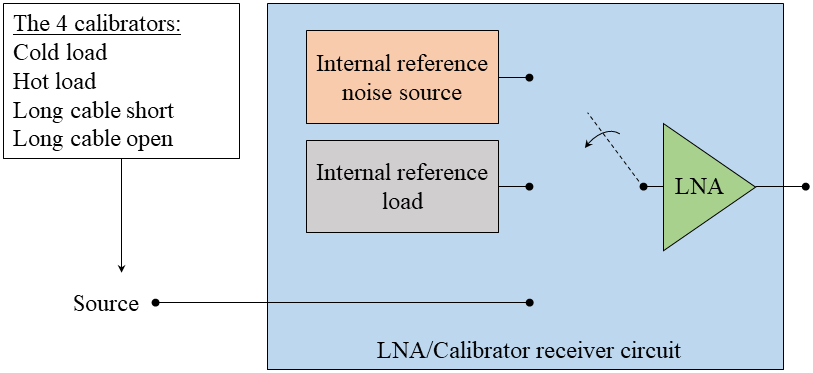
\includegraphics[scale=0.5]{dicke}
    \caption{A diagram of the Dicke switching procedure showing the calibrator position, $50 \Omega$ reference position and reference noise source position. Here, the four canonical calibration sources are used; the ambient and heated $50 \Omega$ loads along with the shorted and open cables. Power spectral measurements of these devices are conditioned by the Low Noise Amplifier (LNA) before being passed on to the spectrometer for initial removal of the time-dependant system gain.}
    \label{fig:dicke}
\end{figure}

The cold load used was taken from an 85033 $50 \Omega$ SMA calibration kit certified by Kirkby Microwave. Multiple heated loads were custom made for this experiment. A simple heated load was constructed from a 4-inch RG-405 coaxial cable terminated with a $50 \Omega$ load attached to a proportional heater connected to DC power with the temperature directly monitored through contact with a thermocouple. As the heated calibration source is typically heated to $\sim 370$ K, which could affect the temperatures of nearby ambient components, an improved calibrator was constructed with the $50 \Omega$ resistor and thermistor attached to a 4-inch semi rigid cable surrounded with thermal insulation and encased in an acrylic cubic shell. A temperature gradient across the 4-inch cable within the construction is produced by the temperature difference between the heated load and the coaxial end connected to the receiver input. As this changes the temperature ‘seen’ by the instrument, a corrective factor is introduced in our calibration calculations and detailed in REFERENCE TEMPERATURE CORRECTION SECTION. While this advanced heated load was used for some of the results presented in this work such as in FORWARD REFERENCE SECTIONS, the simple heated load was the device deployed to the field due to time constraints impacting critical adjustments to reinforce the advanced heated load. A diagram of the advanced heated load is included in \cref{fig:hot_load}.
\begin{figure}
    \centering
    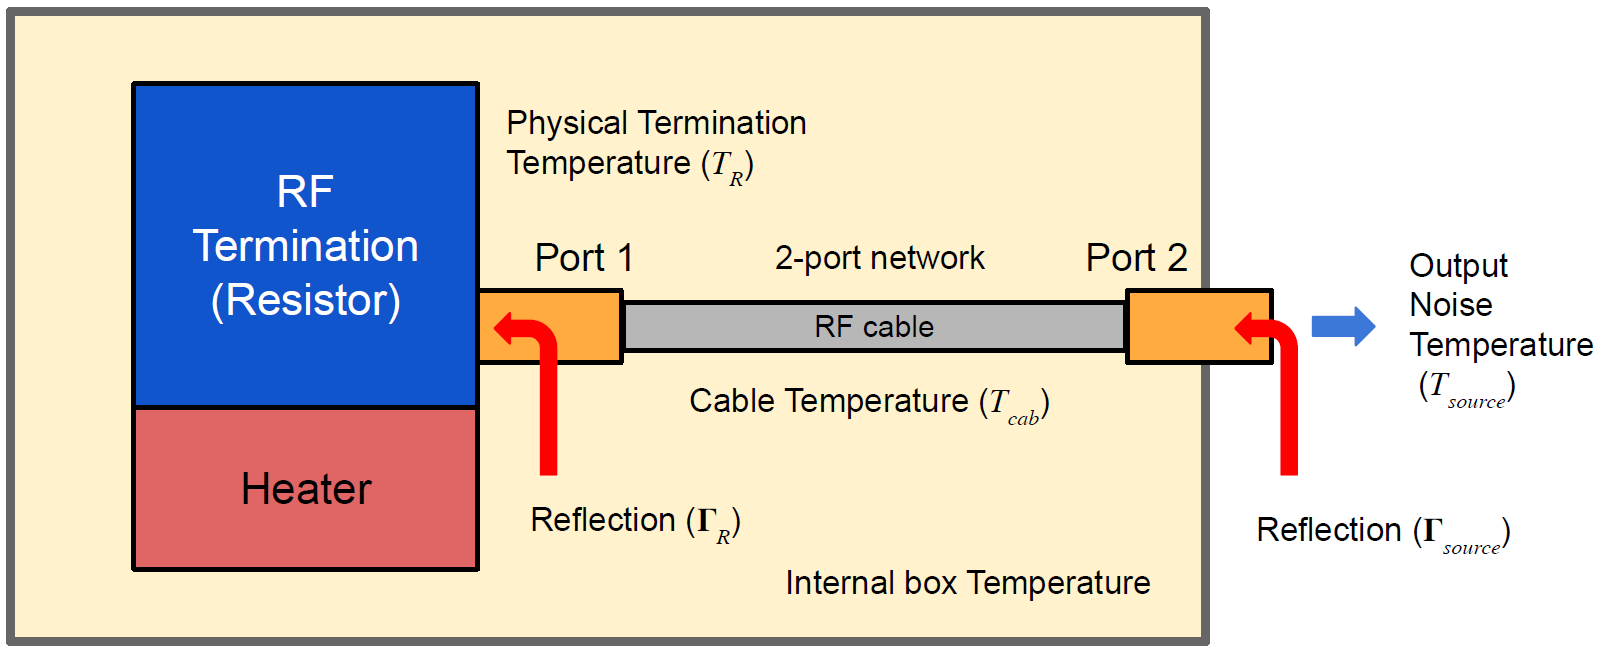
\includegraphics[width=0.65\textwidth]{hot_load}
    \caption{Illustration of the heated load construction for use as a calibration source. The thermally enclosed resistor and powered heater are connected to the input switch via a 4-inch cable as shown in the diagram. These components effectively form a temperature gradient across the calibration device which must be corrected for via the procedure discussed in REFERENCE TEMPERATURE CORRECTION SECTION as $\Tb{R}$, $\Tb{cab}$ and $\Tb{source}$ are not necessarily equal.}
    \label{fig:hot_load}
\end{figure}

Open and shorted coaxial terminations were taken from the same Kirkby 85033 kit and connected to the end of coaxial cables. Over the course of receiver development, many different models and lengths of cables with varied specifications were tried with the final deployed system having the open and shorted ends connected to 10 metre LMC195 coaxial cabling partially built in-house at Cambridge. With the need for more accurate characterisation of the instrument, we have expanded our selection of calibration sources to twelve, maximising the information detailing the instrument response. Additional ambient-temperature $25 \Omega$ and $100 \Omega$ resistors were included for increased data on non-complex impedance response. The same 10 metre LMC195 cable was also terminated with $10 \Omega$ and $250 \Omega$ resistors. An additional 2 metres of LMC195 terminated with $27 \Omega$, $36 \Omega$, $69 \Omega$ and $91 \Omega$ resistors was also included. These additional terminations were all custom made in Cambridge.

The calibration sources and resistances were carefully chosen to permit strategic sampling of the noise waves as a function of impedance. \Cref{fig:smith} demonstrates the extensive scope of frequency-dependent impedances for our calibration sources as well as a simulated impedance of the REACH dipole antenna covering 50--150 MHz.
\begin{figure}
    \centering
    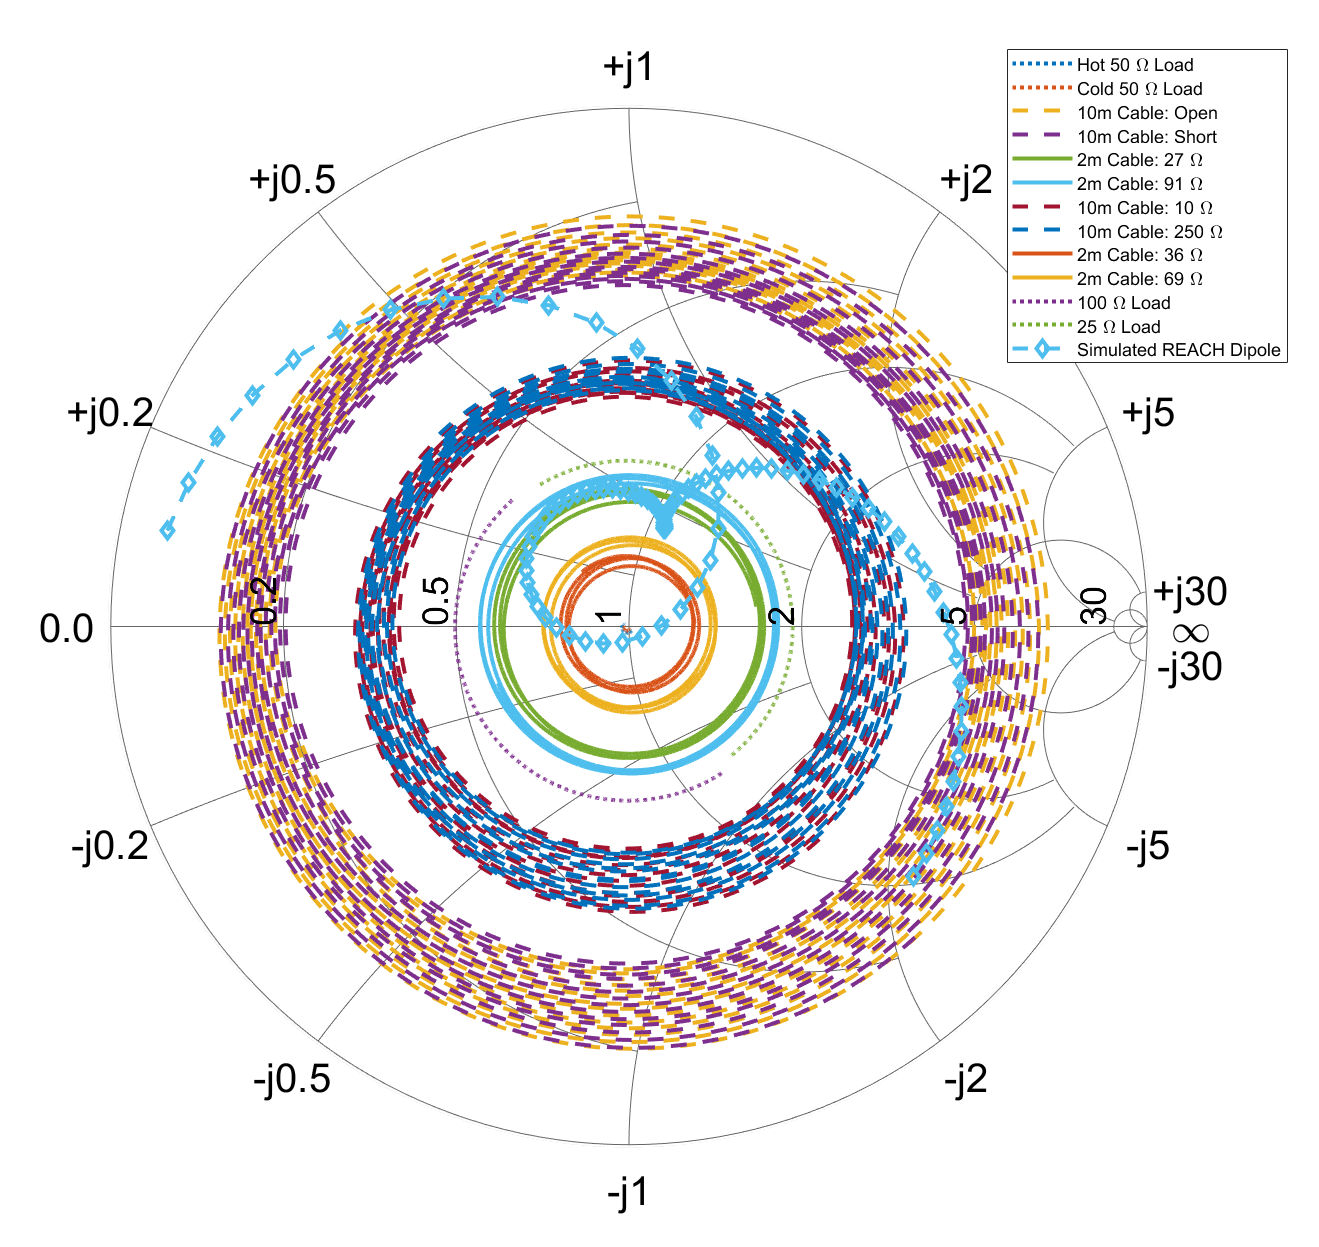
\includegraphics[scale=0.3]{smith}
    \caption{Smith Chart showing the impedance of twelve calibration sources and the simulated REACH antenna (internal variant \#0744) with the centre of the plot indicating an impedance of 50 $\Omega$. The plot ranges from 50--150 MHz with the antenna curve starting at 50 MHz on the left-hand side. The extensive coverage in impedance space by our calibration standards can be interpreted as a substantial amount of information regarding the characteristic response of the instrument. Note that the impedances of the ambient and heated 50 $\Omega$ loads lie directly in the middle of the chart and are partially obscured by the antenna plot. Updated from figure included in REFERENCE REACH NATURE PAPER}
    \label{fig:smith}
\end{figure}
\Cref{fig:smith} also demonstrates measurements of the $25 \Omega$ and $100 \Omega$ loads as half circles on the Smith chart, which differs from the theoretical points at $25 \Omega$ and $100 \Omega$ due to the practical limitations of real-world impedance measurement and exacerbated by the additional RF path in our receiver between the sources and the measurement reference plane for the reflection coefficients. These effects were the motivation for the corrections detailed in REFERENCE S11 CORRECTION MATHS SECTION.

Power spectral measurements are taken of two reference sources for every measurement of a calibration source to divide out the short-time variability in receiver gain as previously stated. Ideally, the reference load would be a separate $50 \Omega$ load of high quality such as from an additional certified calibration kit, but due to time constraints in the deployment, a repeated measurement of the ambient load used as a calibration source was taken. As these Dicke switch measurements detail the changing gain of the system and not the absolute differences between the devices used as calibration sources and reference sources, we believe that this degeneracy would not severely impact the quality of the results presented in this work.

The reference noise source used is a Noisecom NC346A. An important distinction must be made here between the heated $50 \Omega$ load as a calibration noise source and the Noisecom noise diode used as a reference noise source. While the constant noise power provided by the noise diode is necessary for maximal radiometer measurement accuracy through removal of the time-dependent gain fluctuations via the Dicke switching procedure, the direct and accurate measurement of the heated $50 \Omega$ load via thermocouple is beneficial for the removal of systematic noise via accurate noise wave parameter derivation. 

Noise output data of the reference noise diode as provided in decibel excess noise ratio by Noisecom in shown in \cref{tab:ns_noise}.
\begin{table}
    \begin{center}
    \begin{tabular}{ |c|c| }
        \hline
        {Frequency} & {Excess noise ratio} \\
        \hline
        30 MHz & 6.05 dB \\
        40 MHz & 6.03 dB \\
        50 MHz & 6.00 dB \\
        60 MHz & 5.94 dB \\
        70 MHz & 5.91 dB \\
        80 MHz & 5.87 dB \\
        90 MHz & 5.84 dB \\
        100 MHz & 5.79 dB \\
        110 MHz & 5.80 dB \\
        \hline
    \end{tabular}
    \quad
    \begin{tabular}{ |c|c| }
        \hline
        {Frequency (contd.)} & {Excess noise ratio (contd.)} \\
        \hline
        110 MHz & 5.80 dB \\
        120 MHz & 5.77 dB \\
        130 MHz & 5.80 dB \\
        140 MHz & 5.81 dB \\
        150 MHz & 5.83 dB \\
        200 MHz & 5.88 dB \\
        250 MHz & 5.87 dB \\
        350 MHz & 5.87 dB \\
        500 MHz & 5.89 dB \\
        \hline
    \end{tabular}
    \end{center}
    \caption{Manufacturer quoted noise output for the Noisecom NC346A noise diode used as the reference noise source within the Dicke switching procedure as an excess noise ratio. The stability of the noise output within the REACH observational band (50 -- 130 MHz) at these scales should be noted, which is beneficial for the removal of time-dependent system gain.}
    \label{tab:ns_noise}
\end{table}
We can convert the noise output values from \cref{tab:ns_noise} to linear scale using the equation
\begin{equation}
    \mathrm{ENR_{dB}} = 10 \cdot \log_{10} \left( \frac{\mathrm{T} - 290}{290}\right)
\end{equation}
with 290 being the standard reference temperature for noise and $\mathrm{T}$ as a linear-scale excess noise above ambient temperature (assumed to be 298 K). A plot of the linear noise output of the reference noise diode with ambient temperature subtracted is provided in \cref{fig:ns_diode} which may serve as a potential sanity check for our calibration algorithm as these values inform us of the approximate values of the $\Tb{NS}$ noise wave parameter as detailed in REFERENCE RECEIVER MATHS SECTION and verified in REFERENCE NIMA MATLAB RESULTS SECTION. This value may not be exactly replicated however, due to the additional RF path introduced earlier and again detailed in REFERENCE S11 CORRECTION MATHS SECTION. It should also be noted that these values are exclusive to this particular noise source and the use of different noise diodes in future builds, including identical model numbers, would necessarily be different and require recalculation following the above prescription.
\begin{figure}
    \centering
    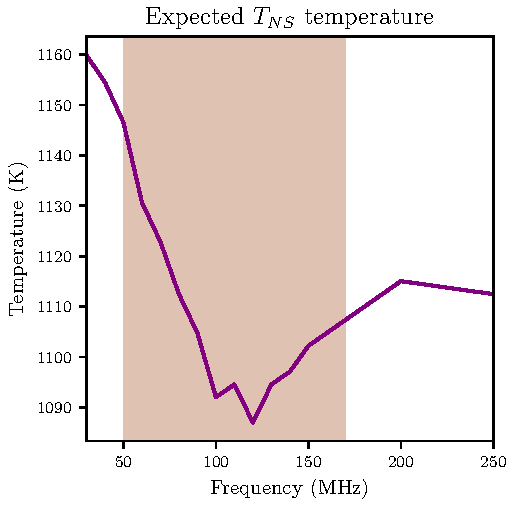
\includegraphics[width=0.5\textwidth]{ns_diode}
    \caption{A plot of the reference noise diode output from the datasheet provided by Noisecom. The scale of the plot gives us a value expected of the $\Tb{NS}$ noise wave parameter from our calibration algorithm. As shown, the output of the diode is essentially stable at these high temperature scales but cannot be measured accurately in the field due to the output being an effective noise temperature from a diode imitating the noise of a black body at such a temperature. The shaded region is the REACH observational band 50--130 MHz.}
    \label{fig:ns_diode}
\end{figure}


% =========================================
\subsubsection{Switches}
The sizeable battery of calibration and reference sources may seem at first glance to run against the primary goal of having a small-volume receiver. To meet this challenge, a complicated network of mechanical switches was conceived to allow for the myriad components and various signal paths through the instrument. The essential calibration sources mentioned in the previous subsection were gathered on an 8-way switch (referred to as MS1) with switch positions one through six taken up by the antenna, cold load, reference noise source, heated load, $25 \Omega$ load and $100 \Omega$ load respectively. To avoid the size requirements of having multiple calibration cables with various terminations, a single 2 metre LMC195 cable and 10 metre LMC195 cable were connected to MS1 positions seven and eight with the opposing ends of the cables connected to their own 4-way switch referred to as MS3 and MS4 respectively. These cable switches were connected to the appropriate terminations according to the previous subsection; $36 \Omega$, $27 \Omega$, $69 \Omega$ and $91 \Omega$ for MS3 positions one through four as well as open termination, shorted termination, $10 \Omega$ and $250 \Omega$ for MS4 positions one through four for the 2 metre and 10 metre cables. A custom 3D-printed structure was designed to house the two calibration cables within the receiver front-end which is highlighted in \cref{fig:stadium}
\begin{figure}
    \centering
    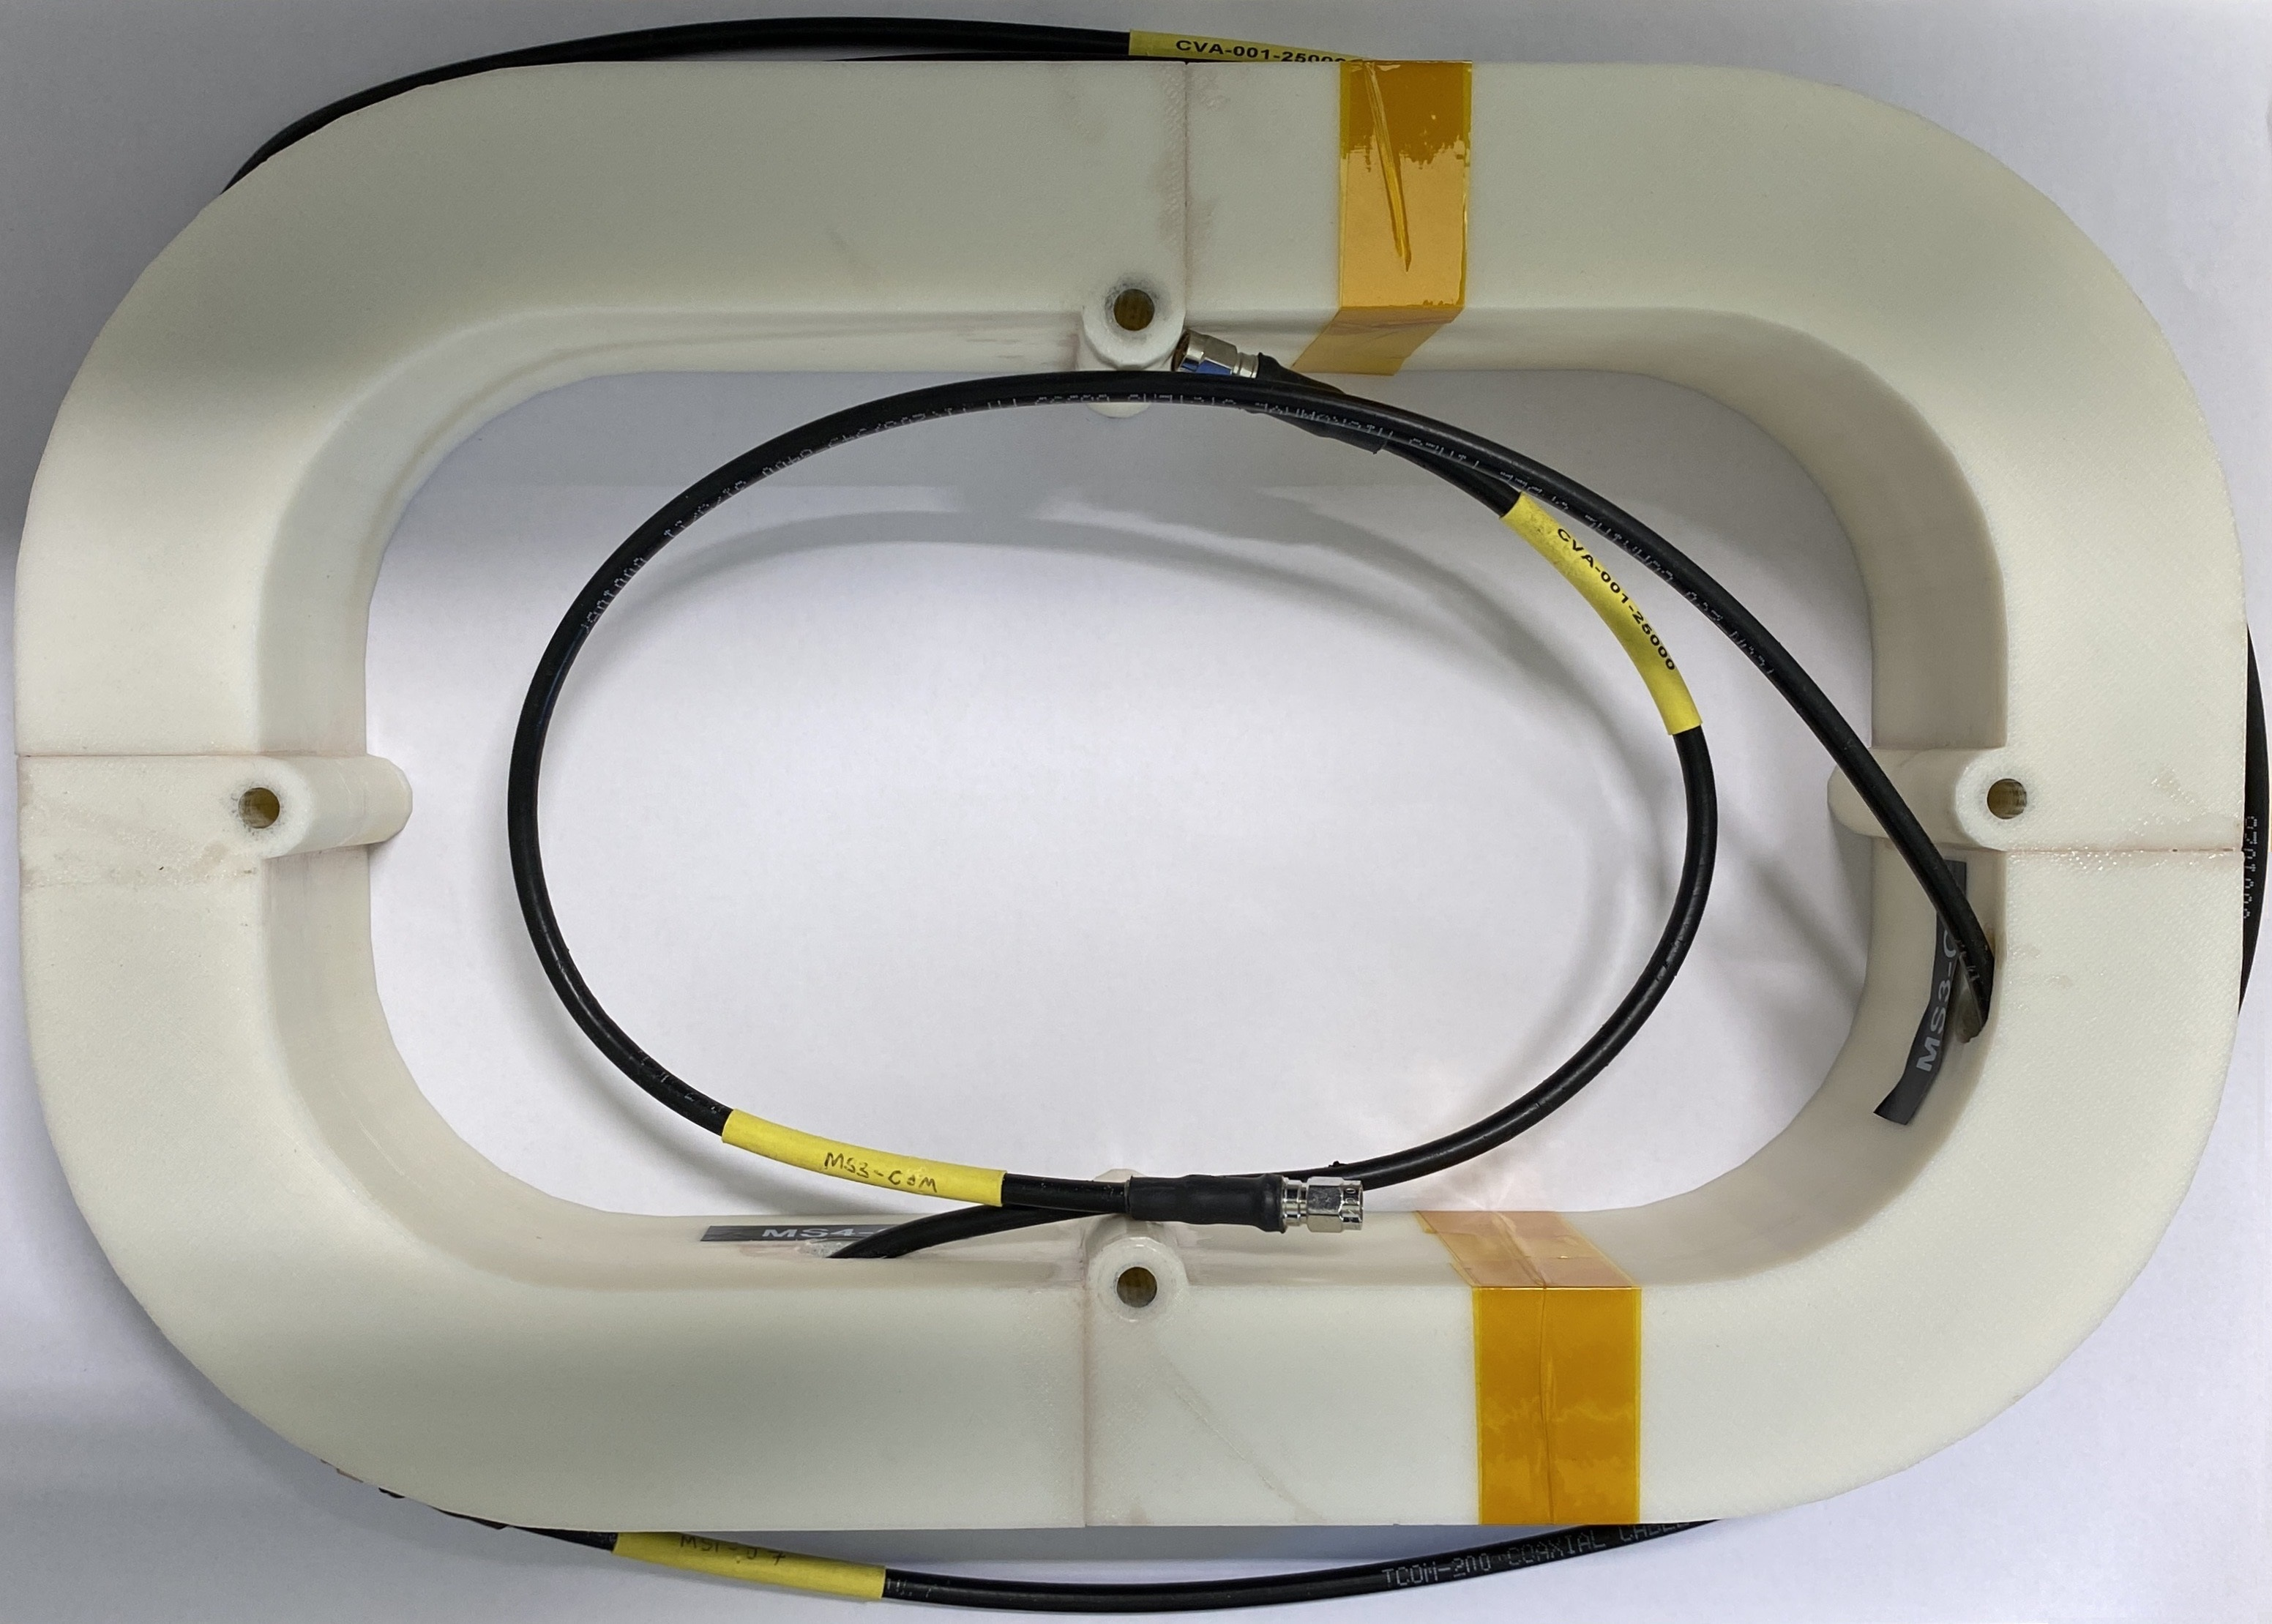
\includegraphics[width=0.65\textwidth]{stadium}
    \caption{3D printed housing for the 2 metre and 10 metre calibration cables. This unit is affectionately referred to as ‘the stadium’.}
    \label{fig:stadium}
\end{figure}

A schematic block diagram of the switching configuration is shown in \cref{fig:overview}.
\begin{figure}
    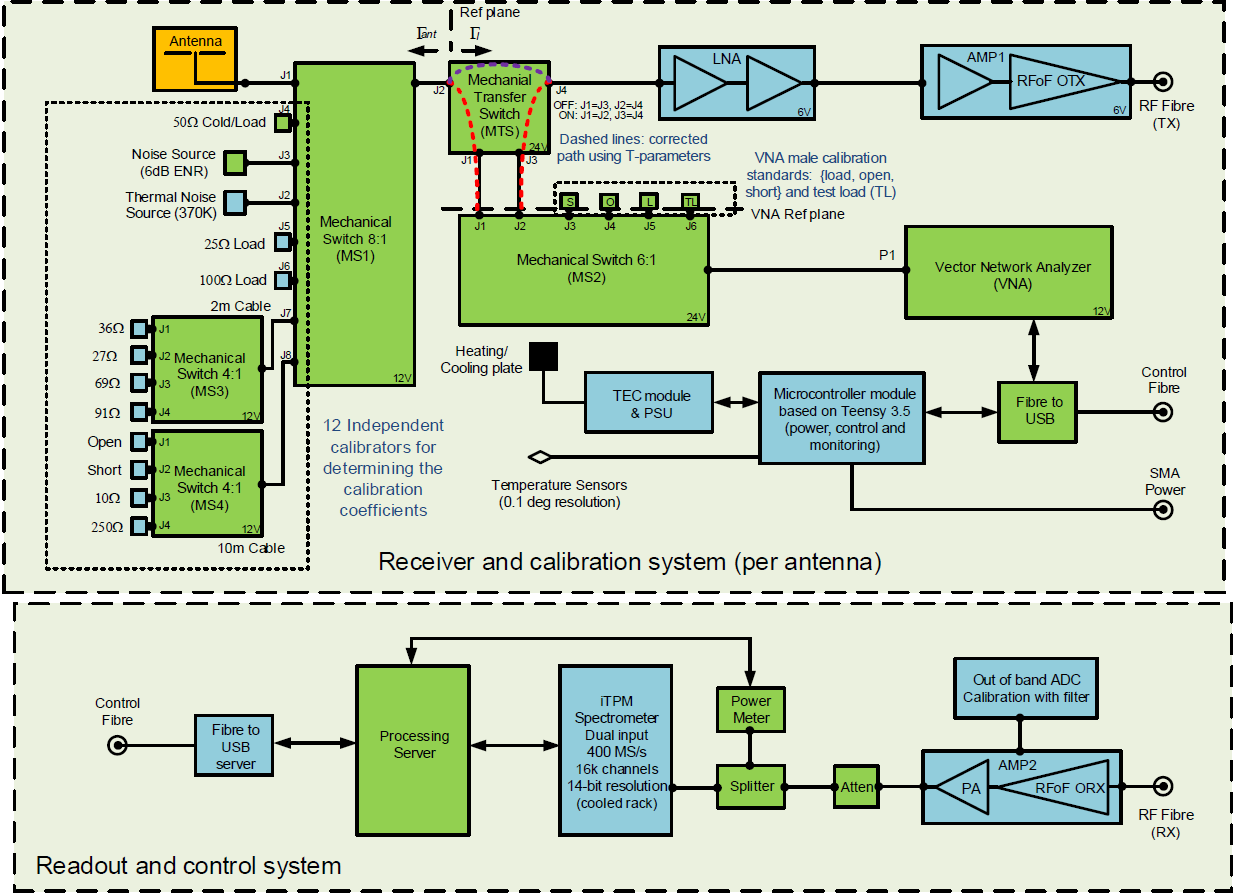
\includegraphics[width=\columnwidth]{radiometer_v8a}
    \caption{An overview of the REACH radiometer showing calibration sources and the antenna connected to an 8-way mechanical input switch at the receiver input. The green sub-blocks represent off-the-shelf components, whilst blue represent custom designs. $\Gamma_{ant}$ represents the reflection coefficient of the antenna or calibrator, $\Gamma_{l}$ is the reflection coefficient of the low noise amplifier (LNA). The red dashed line represents the extra path measured by the VNA that is not present during spectral measurements while the purple dashed line is the path present exclusively during spectral measurements. Corrections for these additional paths are detailed in REFERENCE SPARAMETER CORRECTION SECTION. ‘ENR’ is the Excess Noise Ratio of a Noisecom NC346A noise source; ‘OTX’ indicates an optical transmitter; ‘TX’ indicates transmission mode; ‘TEC’ stands for Thermoelectric Cooling; ‘SMA’ is a SubMiniature version-A connector; ‘PA’ is Power Amplifier; ‘RX’ indicates reception mode and ‘Atten.’ represents a signal attenuator. Updated from figure included in REFERENCE REACH NATURE PAPER OR NIMA PAPER.}
    \label{fig:overview}
\end{figure}
As shown, a Mechanical Transfer Switch (MTS) facilitates pathways to the Low Noise Amplifier (LNA) and Vector Network Analyser (VNA) for spectral and reflection measurements respectively. MTS position two connects directly to the 8-way switch housing the calibration sources and MTS position four leads to the LNA/spectrometer pathway. The first and third MTS switch positions connect to the first two positions of a 6-way switch (MS2) that direct to the VNA. MS2 positions three through six connect to additional calibration standards used to separately calibrate the VNA before measurement as detailed in a following VNA subsection. For all of the connections detailed here, male sources and terminations were connected to female switch connections to avoid reflections that would spawn from the inclusion of male-female adaptors\footnote{or ‘worms’ as they are colloquially referred to.}

An effort was made to reduce any negative effects presented to the instrument by this network of switches. Mechanical switches were implemented over the alternative electronic switches due to the lower signal loss of the former. The Mini-Circuits absorptive switches chosen exhibit 0.01 dB loss within the REACH observational band with better than 100 dB isolation to reduce the radio-frequency leakage into the rest of the signal chain. Extra shielding was added to the switch drivers to further reduce self-induced RFI as shown in \cref{fig:switches}. The 20 mm trace length of the mechanical switch drivers was mitigated by placing the drivers as close to the switch as possible followed with the inclusion of custom 3D-printed connection covers coated with conductive paint.
\begin{figure}
    \centering
    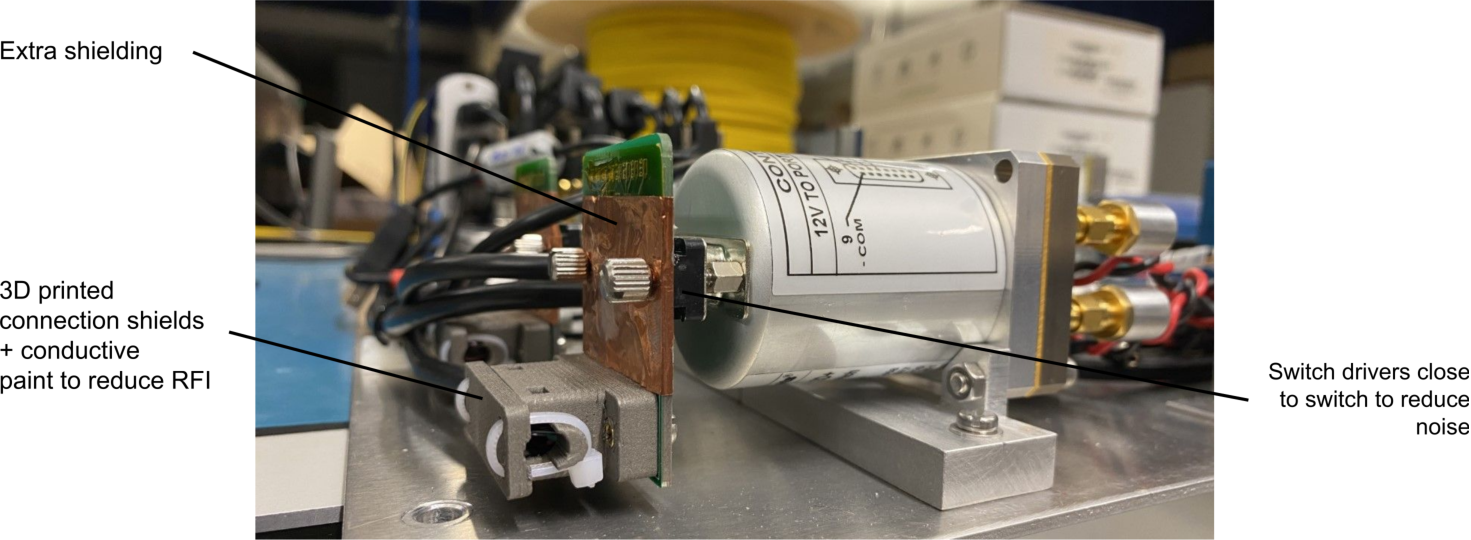
\includegraphics[width=\textwidth]{switches}
    \caption{A mechanical switch installed on the front-end component plate showing the extra shielding, 3D-printed housing and close placement of switch drivers.}
    \label{fig:switches}
\end{figure}
A table of the mechanical switches used is presented in \cref{tab:switches} for reference and a table with the contents of each switch connection detailed in \cref{tab:switch_content}. An mock-up of the switch configuration for a reflection coefficient measurement of the open-ended 10 metre cable is provided in \cref{fig:switch_mock} for illustrative purposes as well.
\begin{figure}
    \centering
    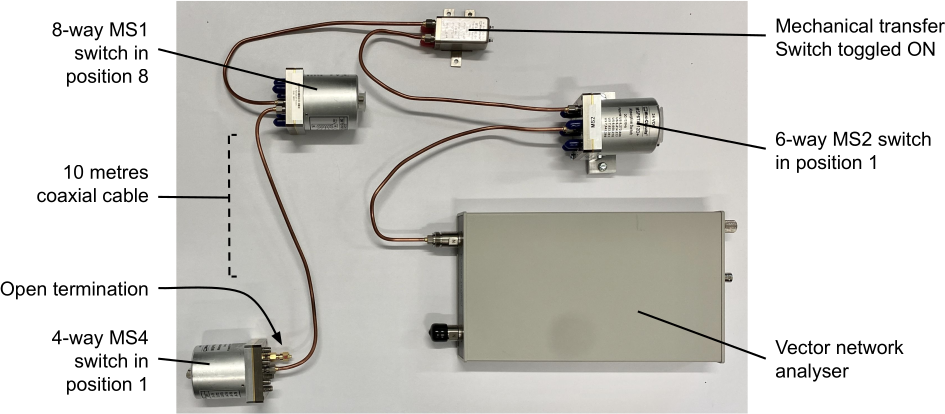
\includegraphics[width=\textwidth]{switch_example}
    \caption{A mock-up of the components and configuration needed for a reflection coefficient measurement of the open-ended 10 metre cable using parts from the receiver (except for the 10 metre cabling which was too long.). For this measurement, the open termination connected to the MS4 switch input port 1 with the MS4 switch toggled to position 1 via command line interface. The MS4 switch output is connected to the 10 metres of LMC195 cabling with the other end of the LMC195 cable connected to the port 8 input of the MS1 switch. The MS1 switch is toggled to position 8 via CLI. The MS1 output connects to the port 2 input of the MTS switch followed by a connection to the port 1 input of the MS2 switch. With the MS2 switch toggled to port 1, the MS2 output should connect to the VNA input allowing for a connection to the opened termination though the MS2, MTS, MS1 and MS4 switches. This configuration allows for a reflection coefficient measurement of the opened termination by the VNA.}
    \label{fig:switch_mock}
\end{figure}


% =========================================
\subsubsection{The microcontroller unit}
As with most modern instruments, control an monitoring of the receiver front-end and its individual components is overseen by a central device. This control unit is required to initialise the specific switch positions needed for measurements as seen in \cref{fig:overview}. As an unmanned experiment in the South African Karoo, the capability for resetting components, especially during remote triage, is another critical function of the controller unit. With 88 necessary connections to oversee within the receiver front-end, construction of an adequate controller using off-the-shelf components would ordinarily take the space of a standardised 19-inch rack ($\sim 48$ cm\textsuperscript{2}). This along with the low noise requirements and restricted power budget of the REACH experiment prompted the development of a novel control unit design; a miniaturised management device or, ‘microcontroller unit’\footnote{Also abbreviated as ‘$\mu$con’ for short.}. Much of the compactness of our miniaturised control unit can be attributed to a careful consideration in constituent components however, an innovative stacked dual-board design allowed us to reduce the size by an order of magnitude condensing the microcontoller unit into a $13 \times 12 \times 10$ cm volume.

The first of the two boards in our microcontroller unit is the control board mounted by a PJRC Teensy 3.5 development board\footnote{Teensy 4.X is suggested for any future receiver designs due to the anticipated permanent reduction in supply of the 90 nm silicon MK64FX512VMD12 chips constituent to the Teensy 3.5. Newer Teensy boards boasting 45 nm chips may also provide increased efficiency and capability in subsequent builds.} based on the Arduino infrastructure. The Teensy board, as shown in \cref{fig:teensy} contains 64 digital input/output ports assigned to individual switch configurations facilitating component control through a USB serial interface.
\begin{figure}
    \centering
    \begin{subfigure}{0.5\textwidth}
        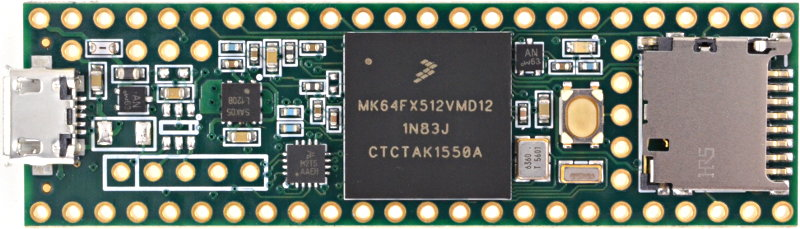
\includegraphics[width=\textwidth]{teensy_top}
    \end{subfigure}
    \begin{subfigure}{0.5\textwidth}
        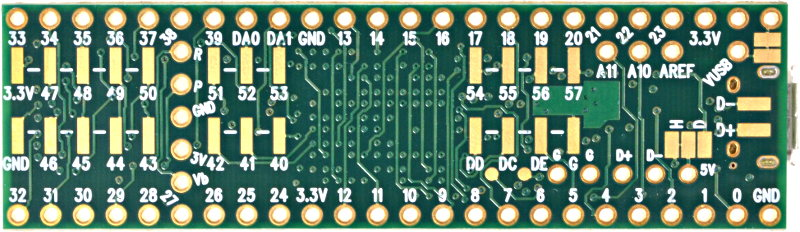
\includegraphics[width=\textwidth]{teensy_bottom}
    \end{subfigure}
    \caption{The front and back of the Teensy board is shown in the top and bottom respectively. Along the edges of the board are the input/output connectors (yellow-outlined white circles) which are paired to specific mechanical switch configurations throughout the front-end.}
    \label{fig:teensy}
\end{figure}
The $110 \times 90$ mm control board upon which the Teensy board is mounted to also contains the 48 V power input from the solar panels as well as 12 V and 5 V outputs for front-end components and can be seen in \cref{fig:control_board}.
\begin{figure}
    \centering
    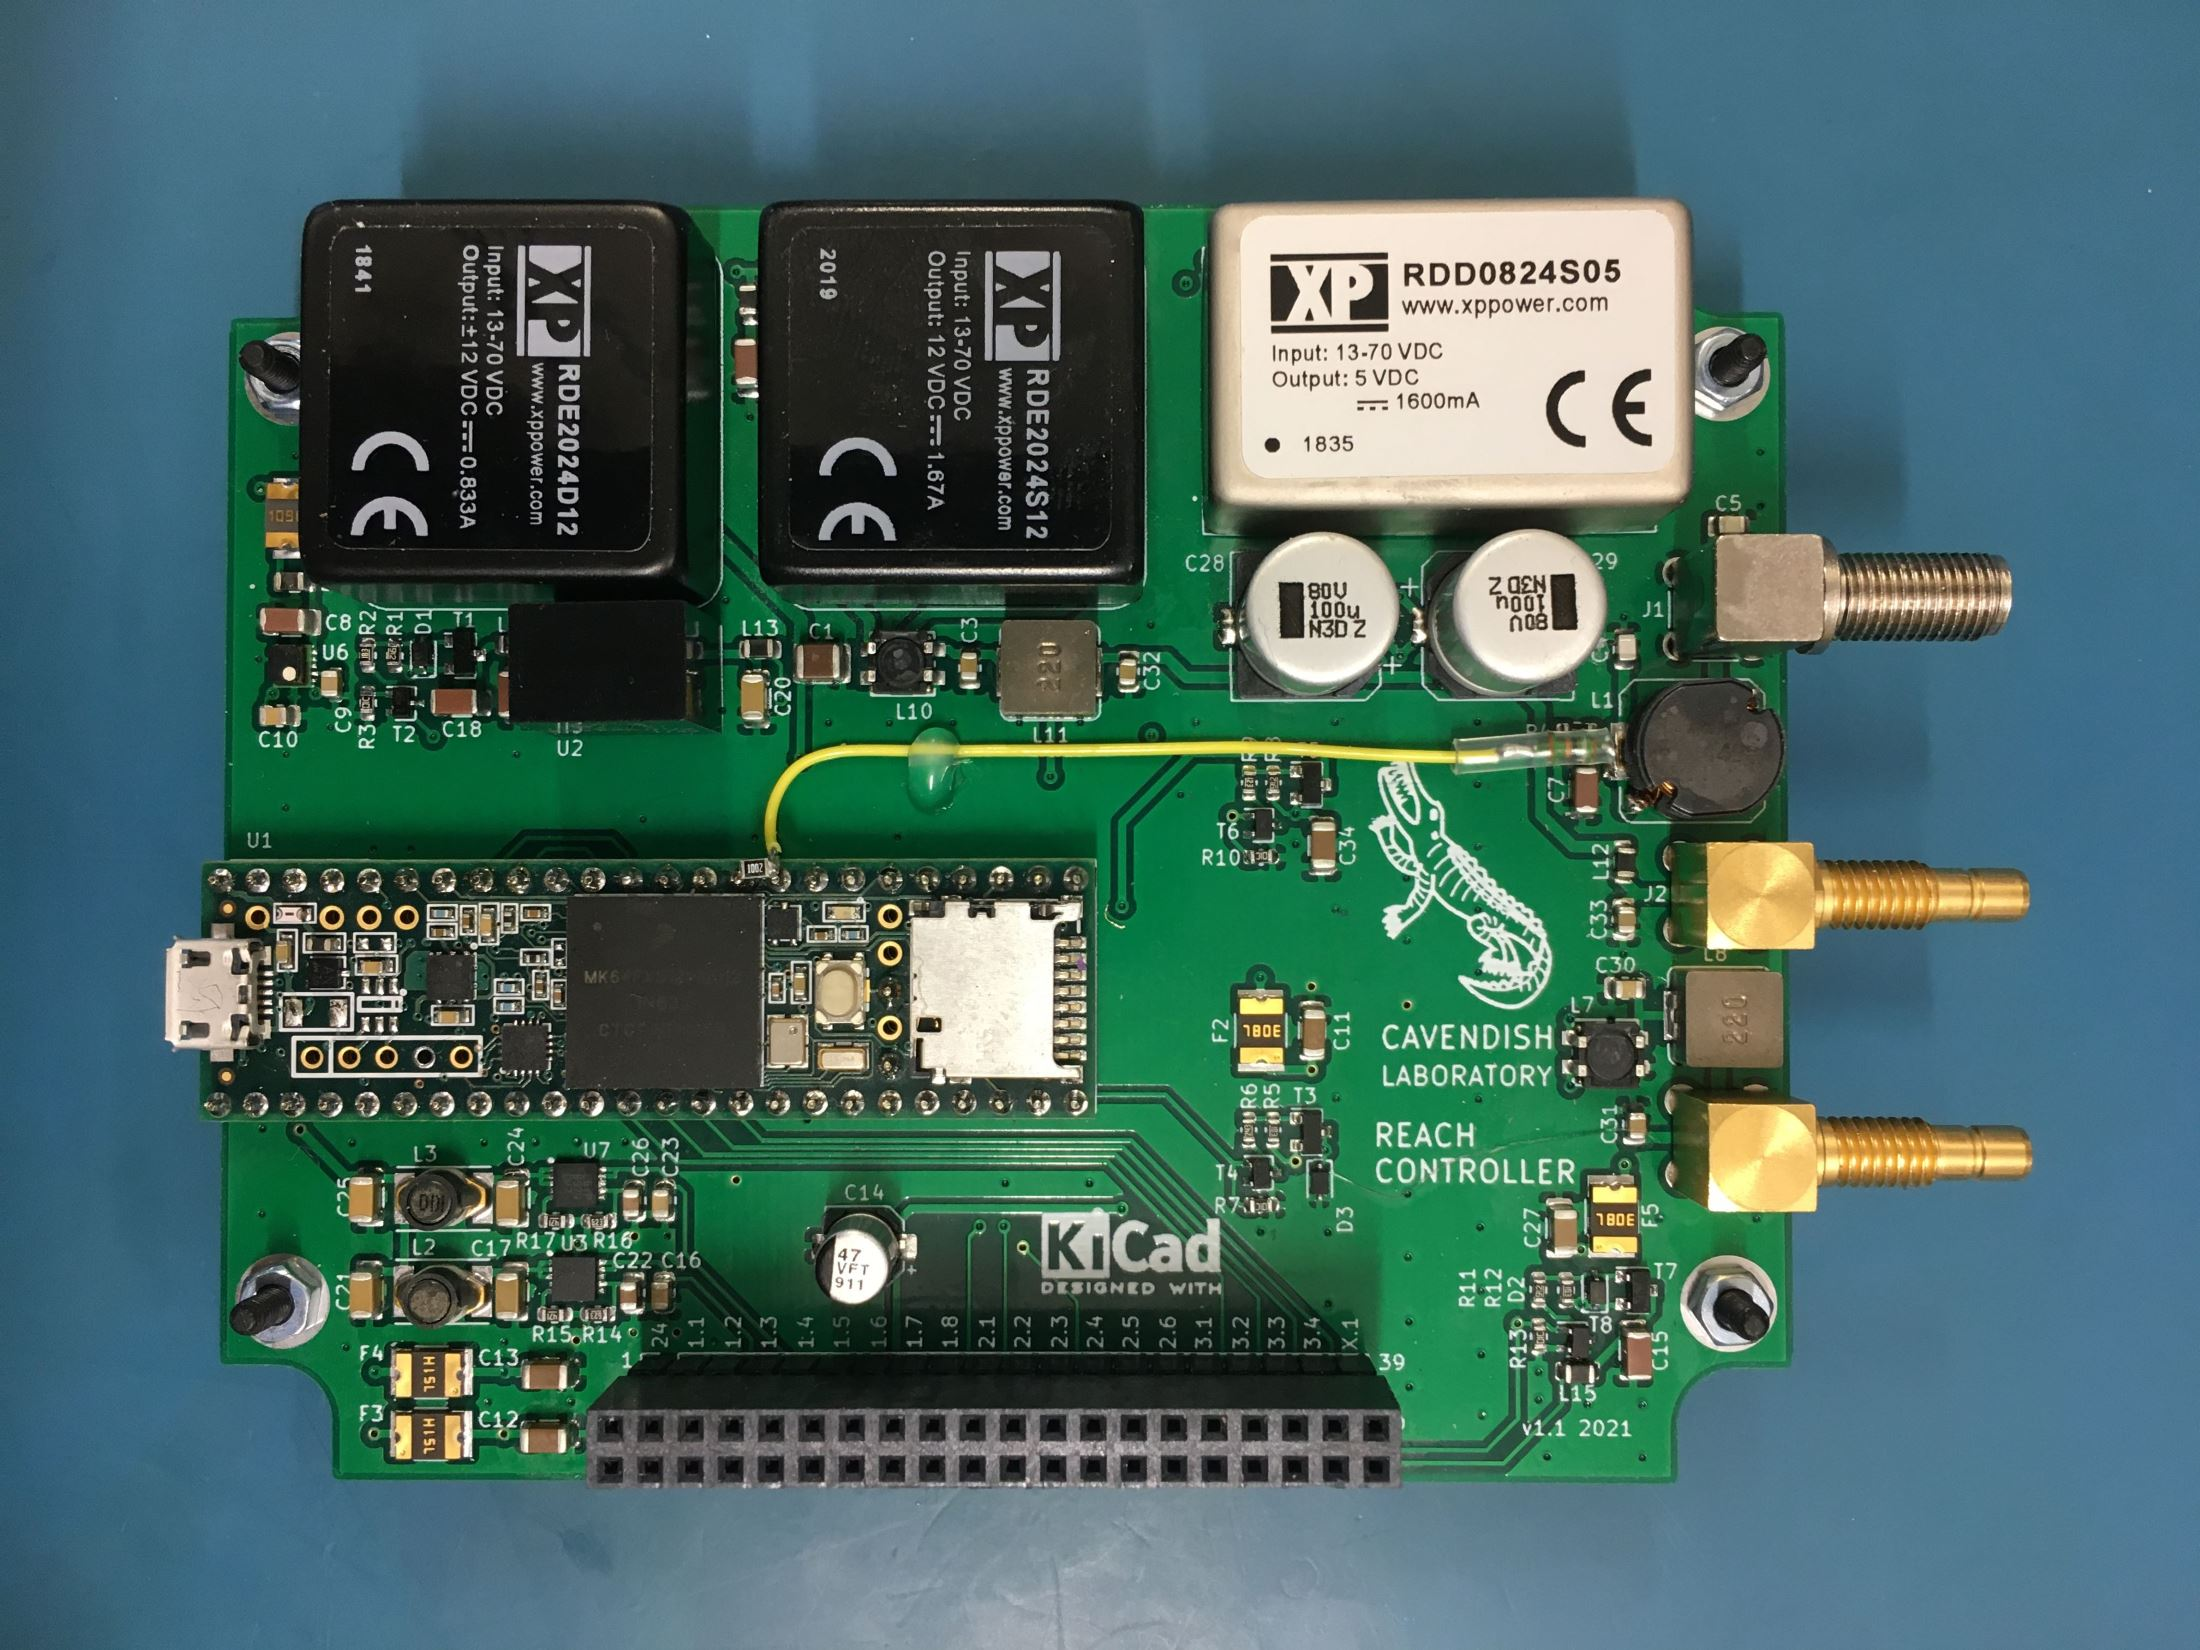
\includegraphics[width=0.5\textwidth]{control_board}
    \caption{The microcontroller unit control board with the Teensy board mounted at the left centre. The 48 V in, 12 V and 5 V out can be seen on the right of the board serving a portion of the overall microcontroller unit's power distribution functionality.}
    \label{fig:control_board}
\end{figure}
The controller board also incorporates RFI filtering and I\textsuperscript{2}C bus subsystems for ancillary device control such as the external fan.

Stacked above the controller board is the breakout board as shown in \cref{fig:break_board} which is primarily responsible for the remaining front-end connections but also a 28 V noise source regulator, 6 V power supply and additional EMI filtering.
\begin{figure}
\centering
    \centering
    \begin{subfigure}{.5\textwidth}
        \centering
        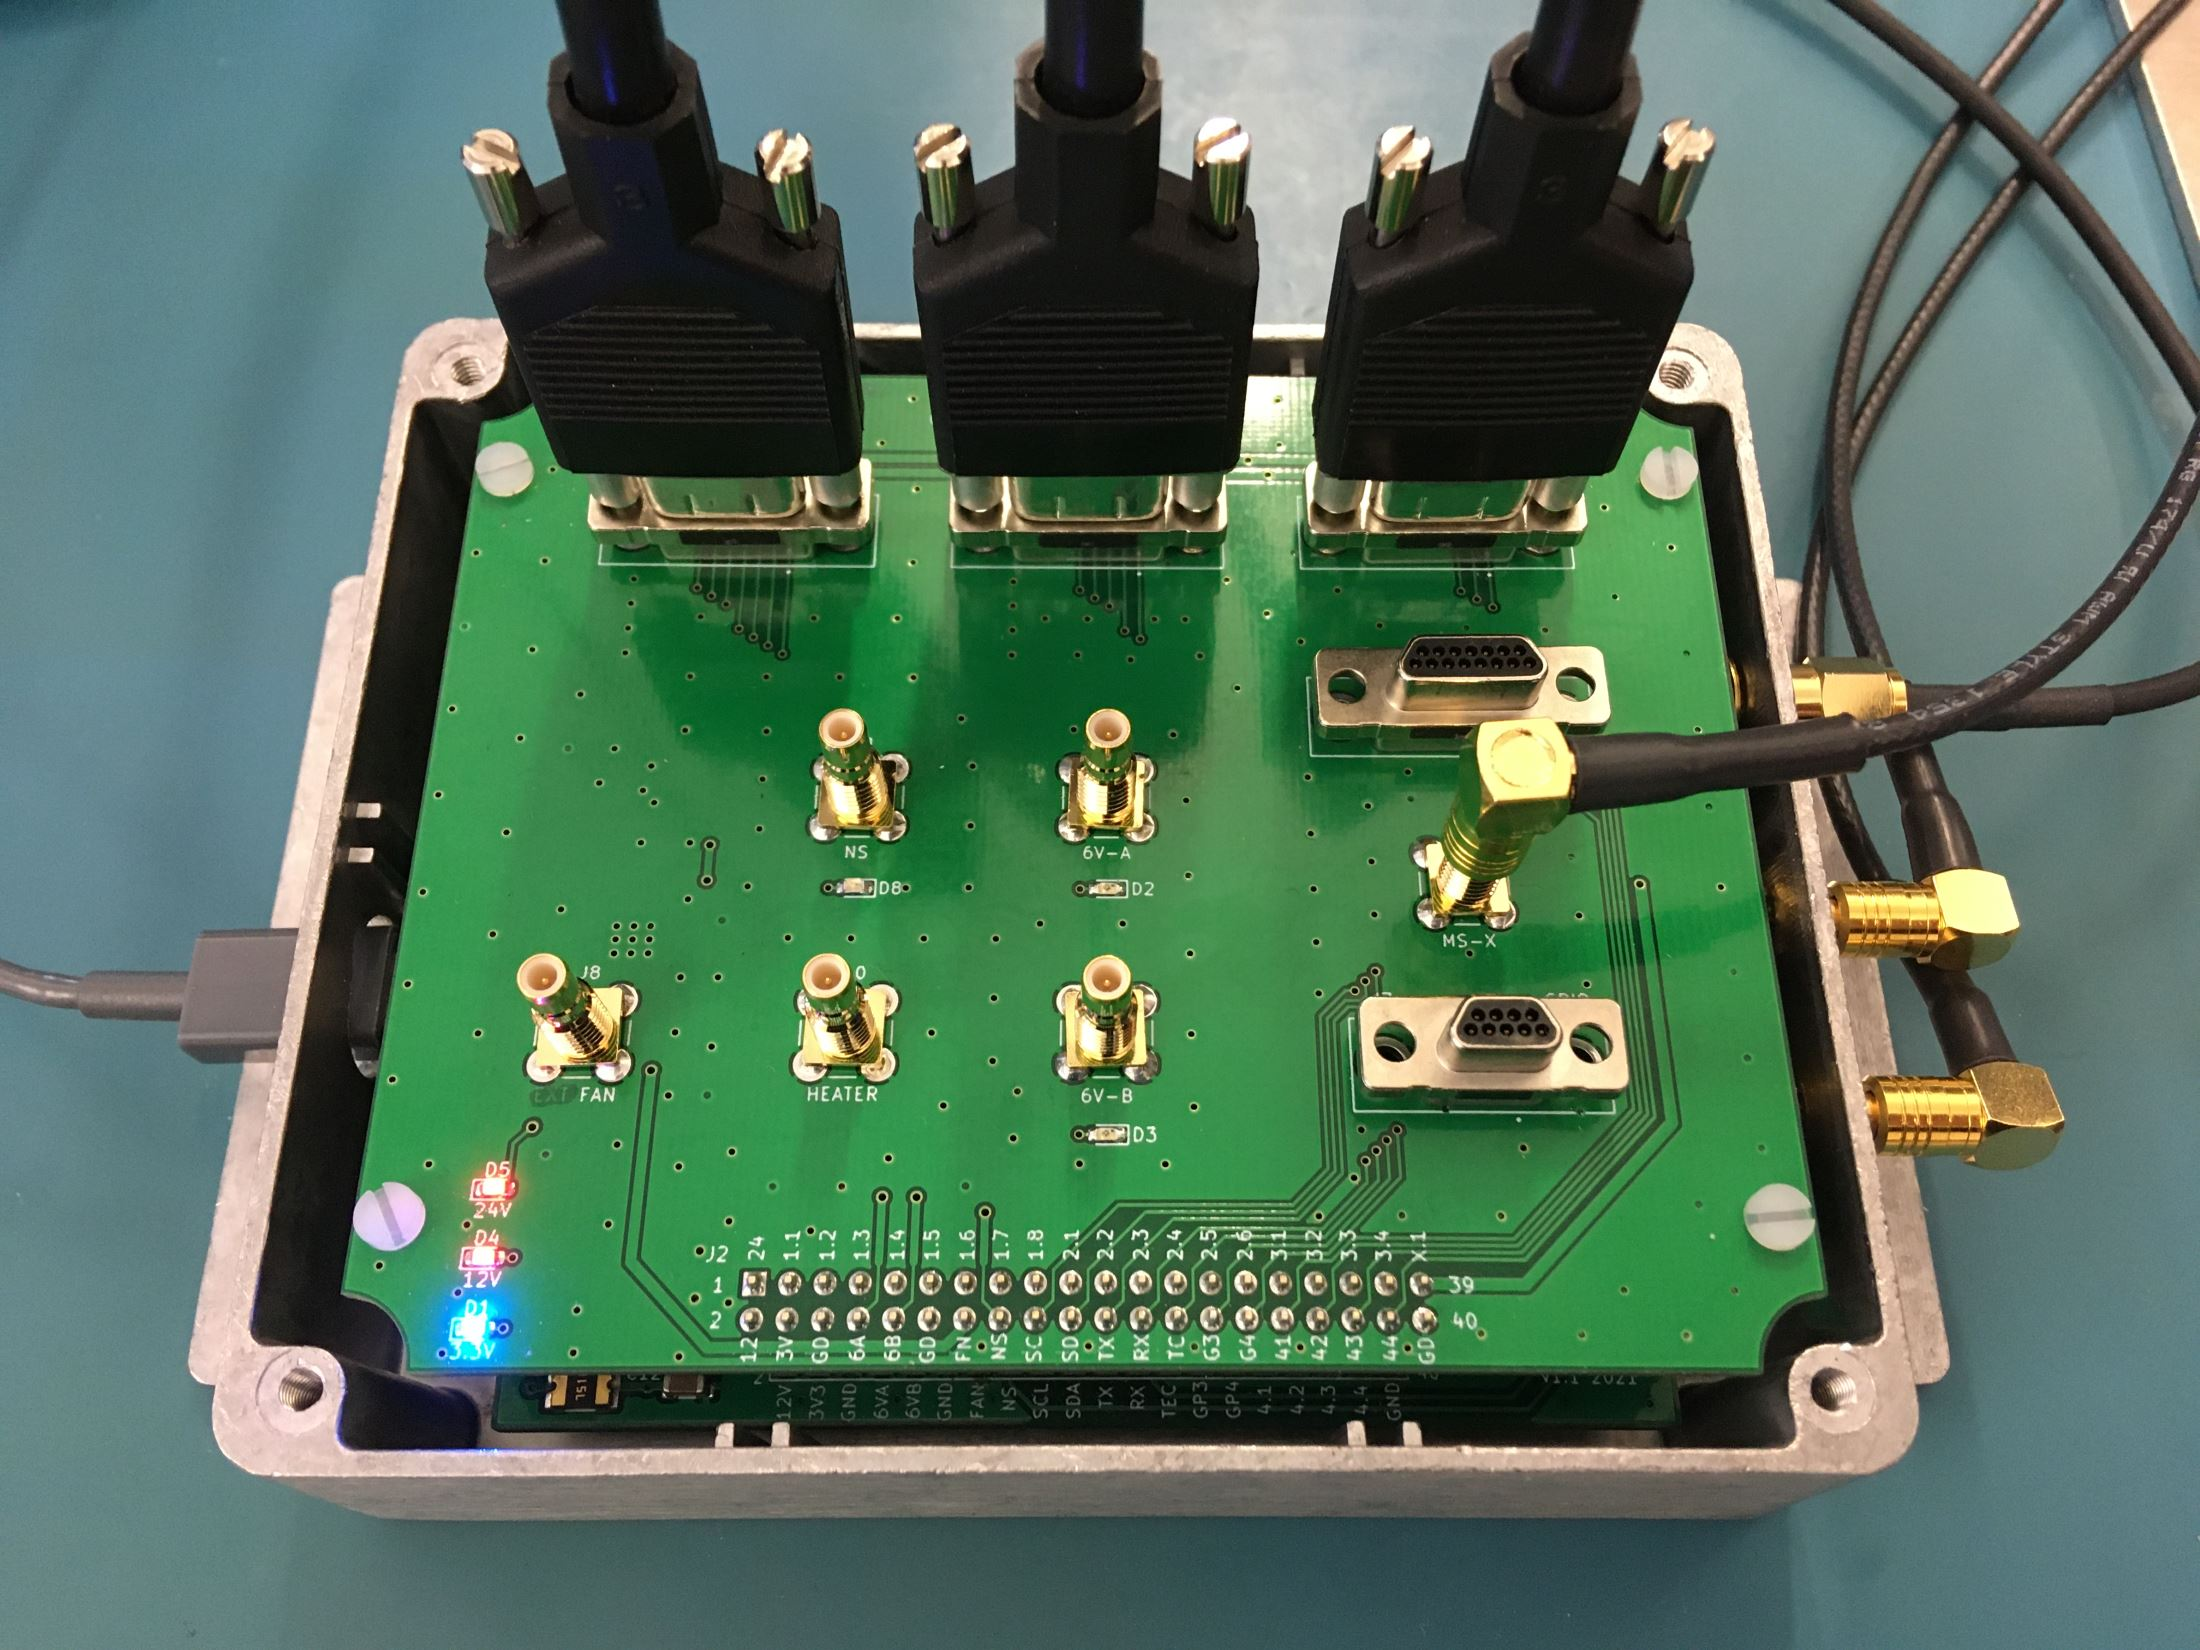
\includegraphics[width=\linewidth]{ucon}
    \end{subfigure}
    \hfill
    \begin{subfigure}{.45\textwidth}
    \centering
        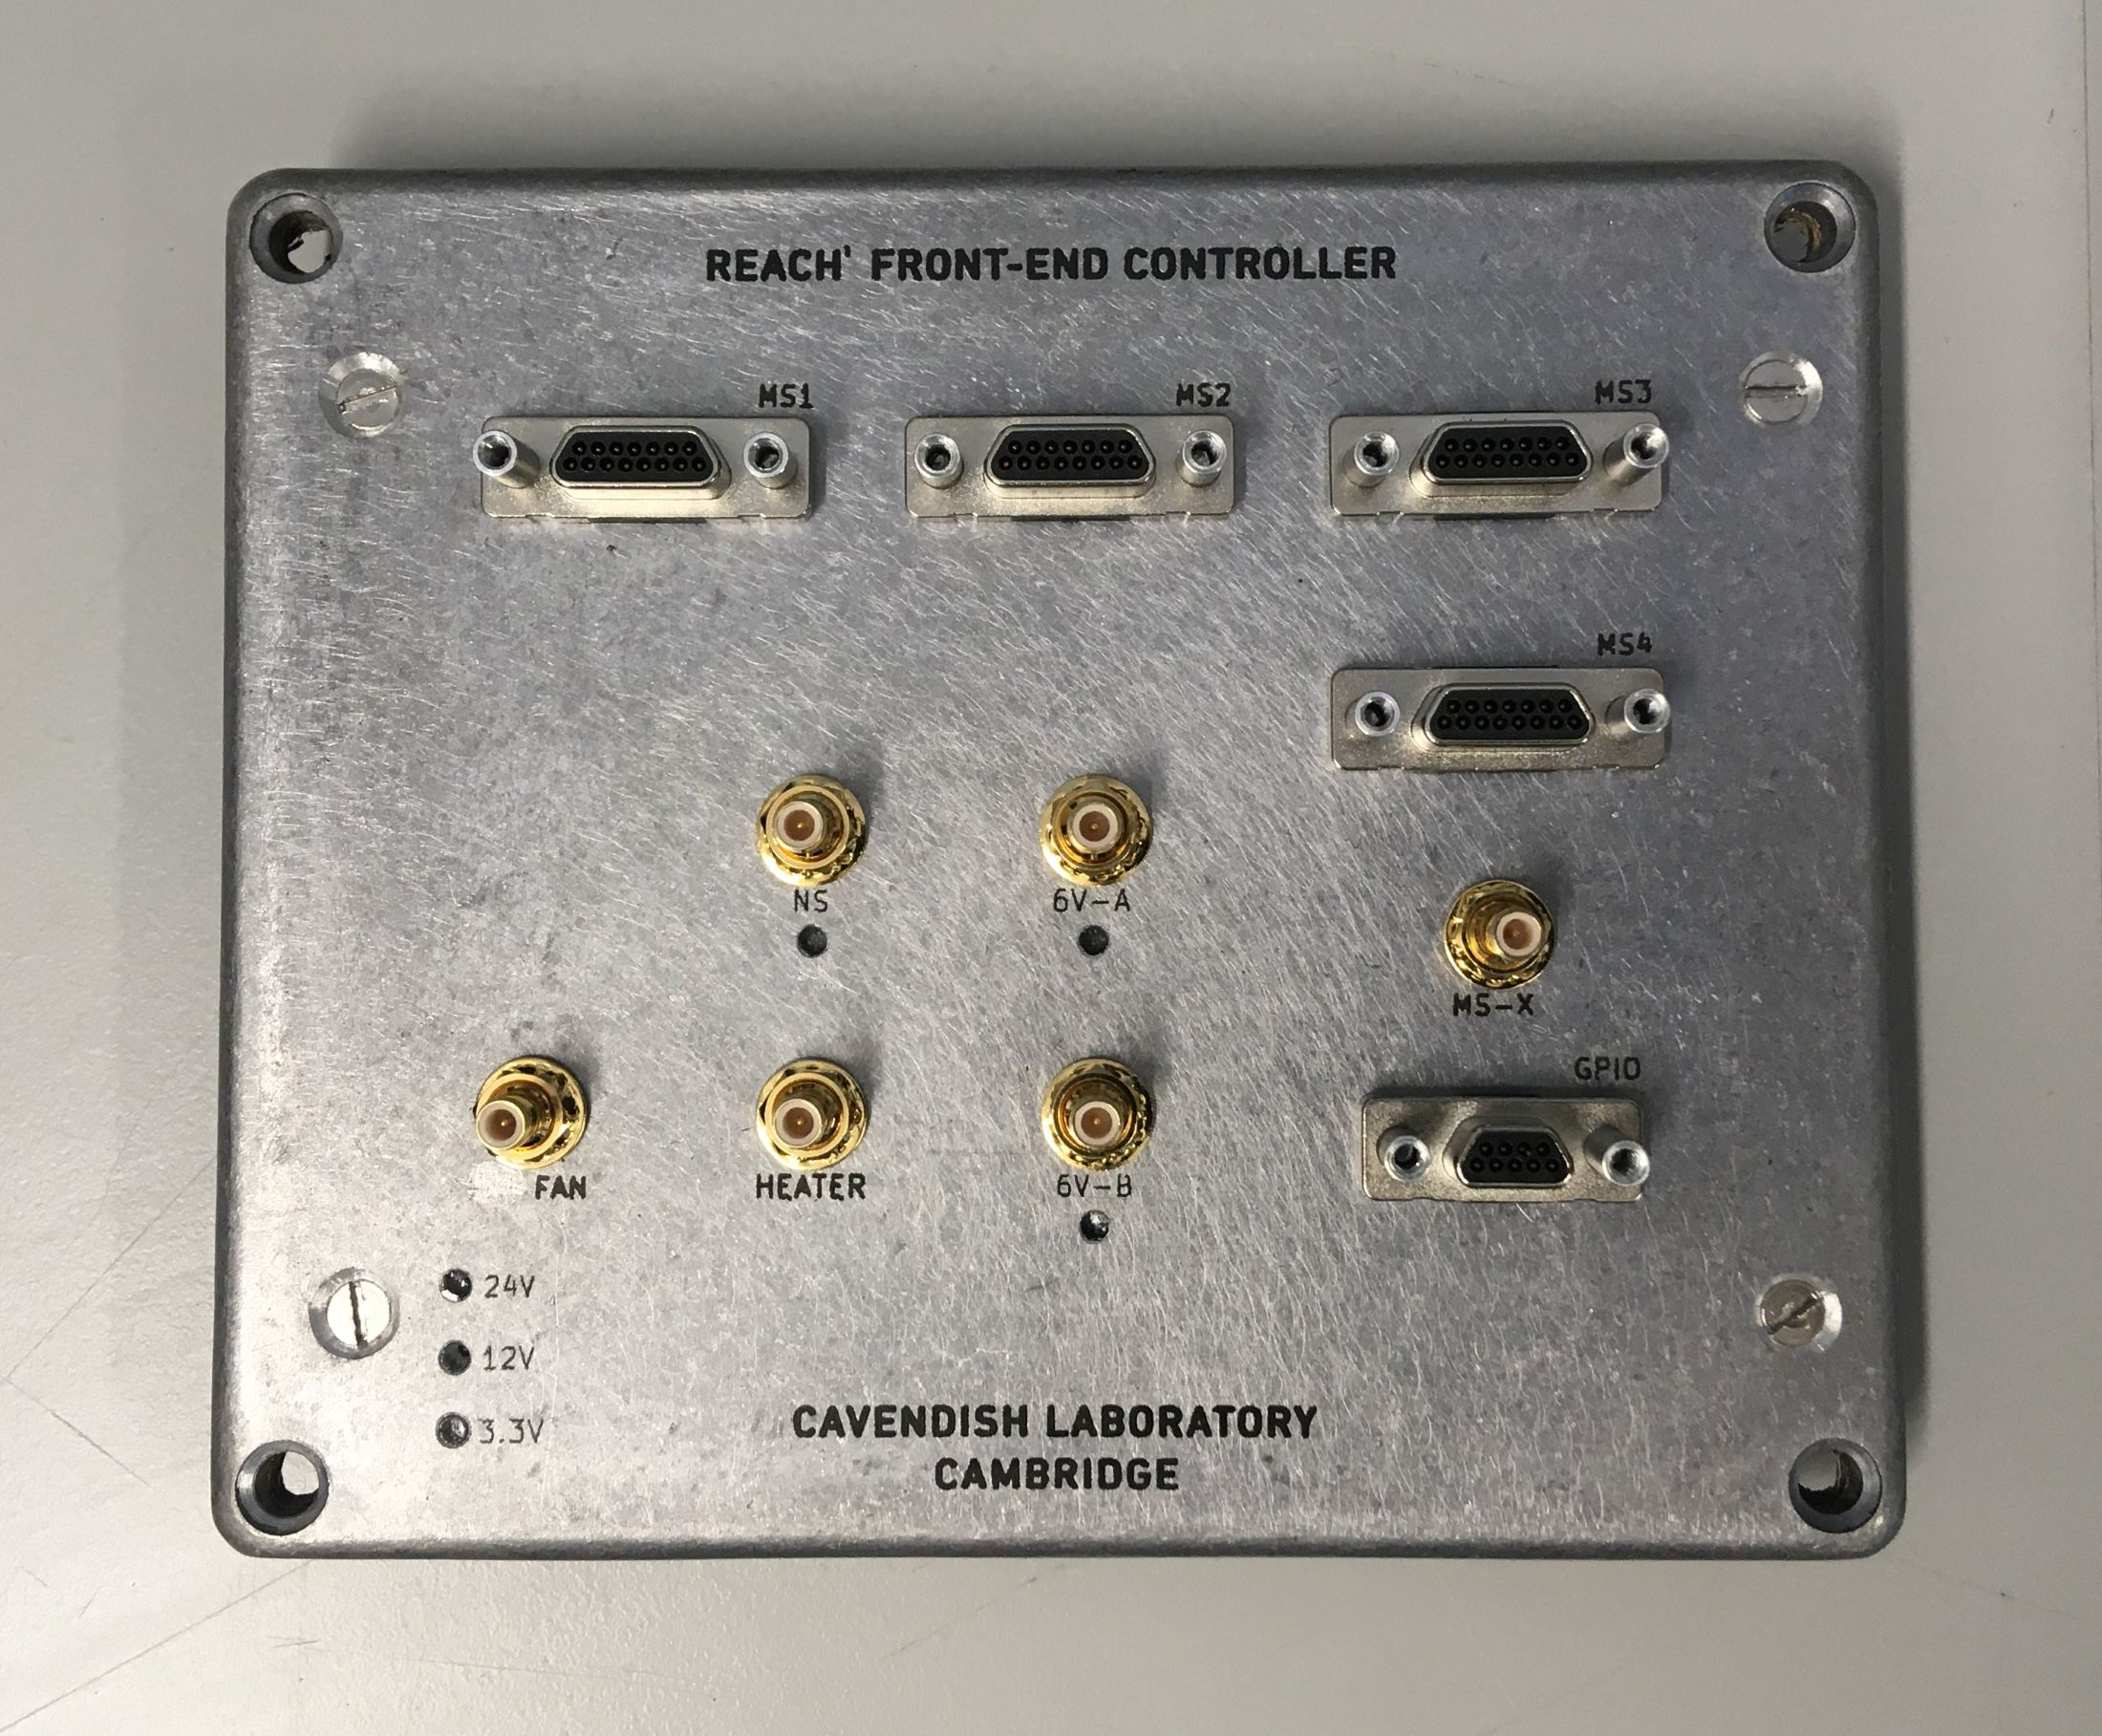
\includegraphics[width=\linewidth]{ucon_cover}
    \end{subfigure}
    \caption{The breakout board of the micocontoller is shown on the right displaying the mechanical switch connections across the top row. The remaining power supply connections can also be seen on the board. The top cover of the completed microcontoller unit is shown on the right with laser markings annotating the connections of the breakout board.}
    \label{fig:break_board}
\end{figure}
A CAD rendering depicting the stacked microcontroller unit is also shown as \cref{fig:ucon_cad}.
\begin{figure}
    \centering
    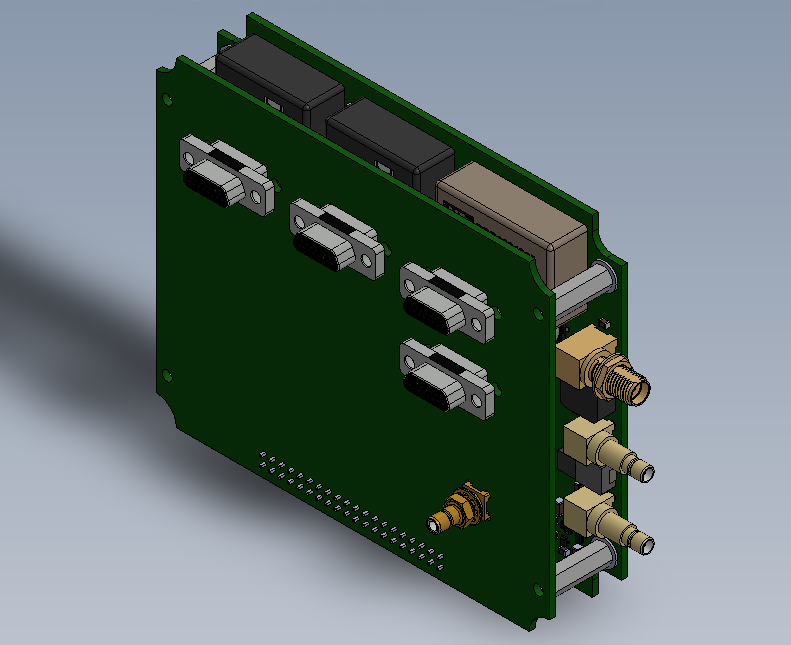
\includegraphics[scale=0.4]{stacked_ucon}
    \caption{A rendering of the micorcontroller assembly showing the breakout board seated above the controller board both outside the microcontroller housing. Also not shown is a heat transfer bracket between the three converter modules. The staked design of the microcontoller allowed for the small form factor required by the REACH experiment.}
    \label{fig:ucon_cad}
\end{figure}
The completed unit supplies power to every component within the front-end except for the thermal management system which has its own power supply unit as previously detailed. A combination of switched-mode power supply (SMPS) and linear regulators are employed to optimise both low noise and efficiency with the six DC-DC power supplies having an efficiency of at least 85\%. A table detailing the power supplies managed by the microcontroller unit is shown in \cref{tab:power_supply}. Further conductive gaskets were placed under bulkhead connectors for additional noise reduction and additional DC filtering is provided on the 48 V input supply. A block diagram of the completed microcontroller unit is provided in \cref{fig:ucon_block}.
\begin{figure}
    \centering
    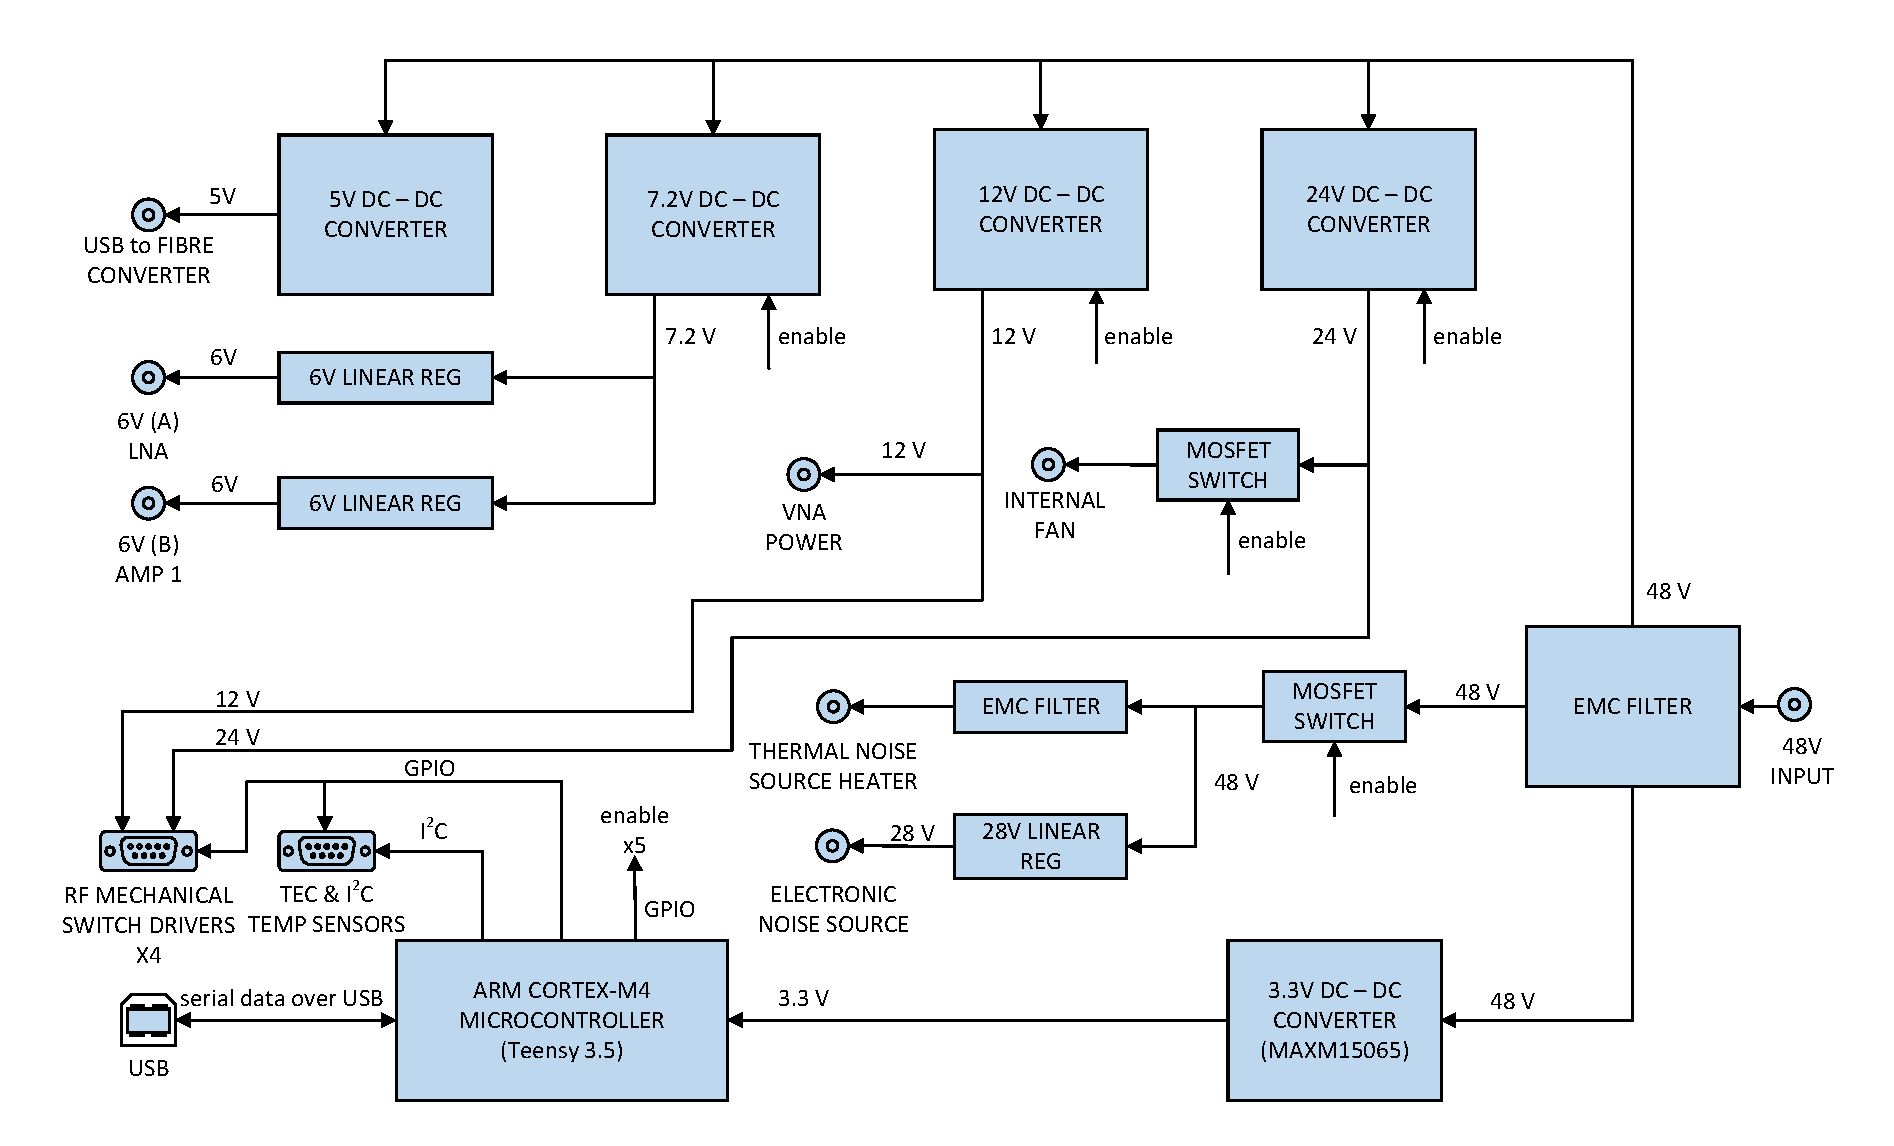
\includegraphics[width=\textwidth]{updated_controller_detail}
    \caption{A detailed microcontroller block diagram showing the components, connections and power considerations incorporated into the design.}
    \label{fig:ucon_block}
\end{figure}
The completed unit demonstrates a high efficiency with a 2 K temperature rise seen within the microcontroller casing with all supplies on at full load.


% =========================================
\subsubsection{Temperature measurement via thermocouple}
Within the receiver front-end are probes measuring the temperatures of various components needed for calibration. Initial designs utilised eight Microchip Technology MCP9808 temperature sensors that communicate directly with the microcontroller unit using I\textsuperscript{2}C protocol over the Arduino command line interface. Thermal gap pads would be used to thermally bond the 2-centimetre-wide temperature sensors to front-end components yielding an accuracy of $\pm 0.5$ K and measured with a cadence of I2C MEASUREMENT CADENCE HERE. The I\textsuperscript{2}C sensors’ native connection to the microcontroller unit conformed to the space restrictions of the front-end enclosure however, it was decided that smaller probe tips for placement on individual components as well as additional temperature sensors would increase the accuracy of our calibration prescription. A Pico Technology TC-08 Thermocouple Data Logger, shown in \cref{fig:tc08}, was employed to accommodate eight more temperature measurements using Pico Technology SE000 K-type thermocouples with TC-08 0.60 mm tip ends thermally bonded to components using RTV Thermally Conductive Oxime made by Electrolube.
\begin{figure}
    \centering
    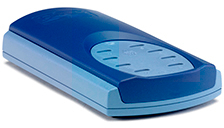
\includegraphics[width=0.4\textwidth]{tc08}
    \caption{The Pico Technology TC-08 Thermocouple Data Logger for use with eight K-type thermal probes.}
    \label{fig:tc08}
\end{figure}
The simple incorporation of the TC-08 with our receiver automation software through the manufacturer’s proprietary Python libraries also factored into our decision to use the device. The TC-08 thermocouples have an accuracy of $\pm 1.1$ K\footnote{Sum of $\pm0.2$\% of reading and $\pm0.5$ K according to manufacturer specifications.} for our measurements typically around 300 K and relay information to the back-end server via USB connection at a cadence of one measurement every 10 seconds. A table of the TC-08 Data Logger port assignments is shown in \cref{tab:tc08}\footnote{These port assignments are representative of the front-end configuration at the time of shipment to South Africa in December 2022 and are subject to change.}.
\begin{table}
    \begin{center}
    \begin{tabular}{ |c|c| }
    \hline
    TC-08 Port Number & Component \\
    \hline
    Port 0 & Cold Junction \\
    Port 1 & MS1 switch \\
    Port 2 & Heated load thermistor \\
    Port 3 & MS3 switch\\
    Port 4 & MS4 switch \\
    Port 5 & 2 metre calibration cable \\
    Port 6 & 10 metre calibration cable \\
    Port 7 & Low noise amplifier \\
    Port 8 & Antenna (laboratory) \\
    \hline
    \end{tabular}
    \caption{The port assignments for the TC-08 connecting to various components within the receiver front-end. The Port 2 thermocouple was attached to the thermistor end of the simplified heated load construction. The Port 5 and 6 probes were connected directly to the outside of the calibration cables for measurement of the physical cable temperature with the terminating sources assumed to be at the same temperature as their respective switches. In the Cambridge laboratory, the Port 8 thermocouple was fed through a small hole drilled through the wall of the front-end enclosure and attached to the end of a makeshift antenna used for testing of the calibration algorithm.}
    \label{tab:tc08}
    \end{center}
\end{table}

We highlight that Port 0 of the TC-08 lists a “Cold Junction” which is the temperature of the Data Logger unit itself and not the similarly named ambient temperature “cold” load. Furthermore, the position of the MCP9808 I\textsuperscript{2}C temperature sensors were not finalised or thermally bound to anything by the time of deployment in August 2023 though it is envisioned that measurements of additional components needed for the temperature corrections detailed in TEMPERATURE CORRECTIONS CHAPTER are the primary responsibility of the I\textsuperscript{2}C sensors. The temperature stability of various sources recorded by the TC-08 are shown in \cref{fig:temperature}.
\begin{figure}
    \centering
    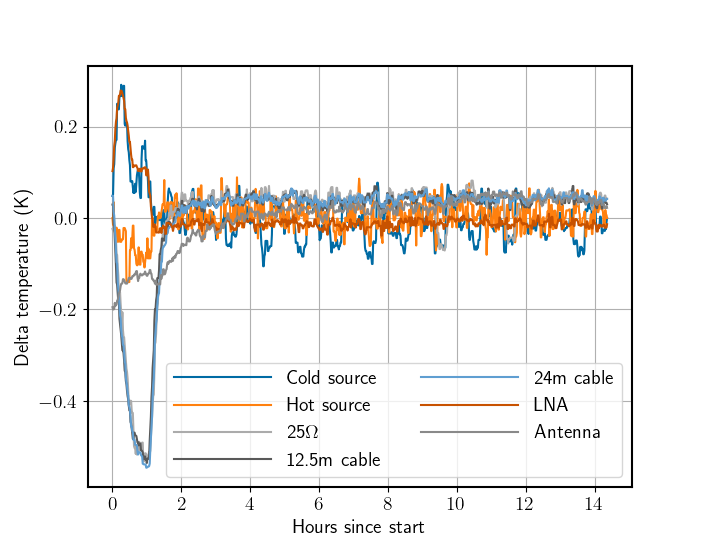
\includegraphics[scale=0.6]{temperature}
    \caption{Receiver component temperature stability recorded by the TC-08 Data Logger. The fluctuations seen within the first two hours of the measurements are from the initiation of the thermoelectric cooler and its attempt to stabilise the front-end internal temperature. We highlight the temperature stability of the individual components after environmental stability is achieved. The plot includes measurements of the 12.5 metre and 24 metre calibration cables before being replaced by the 2 metre and 10 metre cables as detailed in Calibration sources subsection.}
    \label{fig:temperature}
\end{figure}


% =========================================
\subsubsection{Vector Network Analyser}
Reflection coefficients of the calibration sources, LNA and antenna are measured with a Copper Mountain Technologies TR1300/1 2-port 1.3 GHz vector network analyser (VNA) shown in \cref{fig:vna}.
\begin{figure}
    \centering
    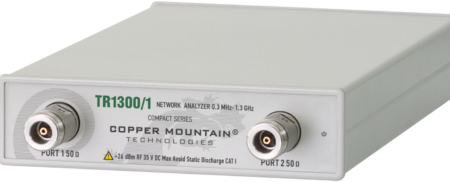
\includegraphics[scale=0.5]{vna}
    \caption{Copper Mountain Technologies TR1300/1 Vector Network Analyser. Image taken from Copper Mountain Technologies website.}
    \label{fig:vna}
\end{figure}
The main consideration for including this VNA model was the small $28.5 \times 14.2 \times 4$ cm form factor for inclusion in the front-end enclosure. The VNA measurement accuracy as provided by the manufacturer is shown in \cref{tab:vna_acc}.
\begin{table}
    \begin{center}
    \begin{tabular}{ |c|c| }
    \hline
    Reflection measurement & Accuracy (Magnitude) \\
    \hline
    -15 dB to 0 dB & $\pm$0.4 dB \\
    -25 dB to -15 dB & $\pm$1.5 dB \\
    -35 dB to -25 dB & $\pm$4.0 dB \\
    \hline
    \end{tabular}
    \caption{Manufacturer quoted measurement accuracies for the Copper Mountain Technologies TR1300/1 Vector Network Analyser.}
    \label{tab:vna_acc}
    \end{center}
\end{table}

Reflection coefficient measurements of various receiver components is shown in \cref{fig:s11_meas}. 
\begin{figure}
    \centering
    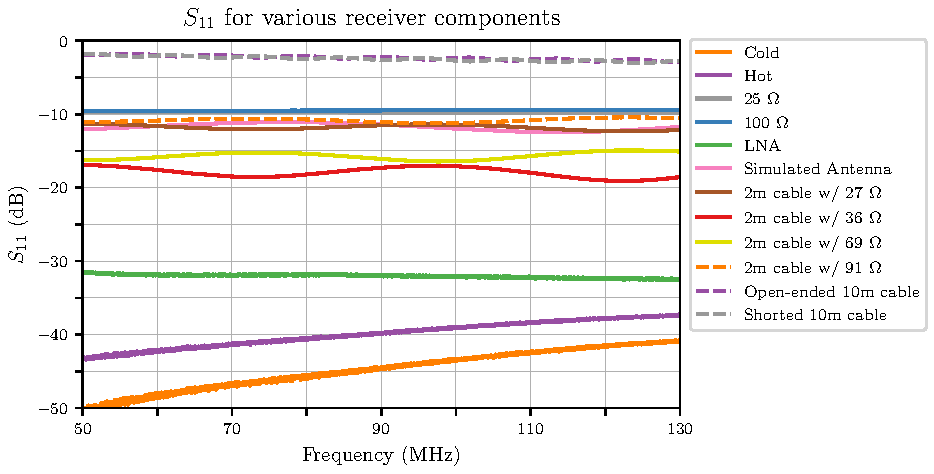
\includegraphics[width=\columnwidth]{s11_meas}
    \caption{Reflection coefficients for various receiver components including the LNA and simulated antenna.}
    \label{fig:s11_meas}
\end{figure}
Upon inspection of \cref{tab:vna_acc}, one may note that the VNA is not rated for extremely low reflection measurements below -35 dB such as the ambient temperature and heated $50\Omega$ loads shown in \cref{fig:s11_meas}. In order to quantify the quality of our measurements in this low-reflection regime, we use the manufacturer provided data of \cref{tab:vna_acc} and calculate a spread in $\pm$dBs representing our measurement error for the regions our machine is rated for. We then convert this spread from dB to linear using
\begin{equation}
    \mathrm{measurement \ spread} = 10^{\frac{\mathrm{measurement} + \mathrm{error}}{10}} - 10^{\frac{\mathrm{measurement} - \mathrm{error}}{10}}
    \label{eq:vna_spread}
\end{equation}
The linear measurement spreads are plotted in \cref{fig:vna_acc} where we have fitted the manufacturer provided data with a decaying exponential using \textsc{SciPy.optimize} and extrapolated to the ranges applicable to the 50$\Omega$ loads. \begin{figure}
    \centering
    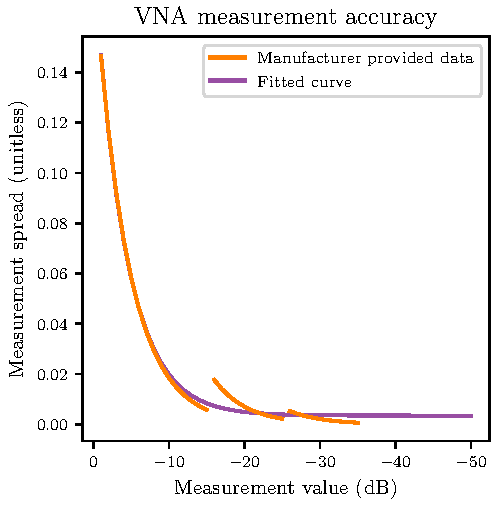
\includegraphics{linear_vna_accuracy}
    \caption{VNA measurement spreads on a linear scale as a fraction of reflected power representing the measurement accuracy of the machine. Manufacturer provided data are shown in orange. A best-fit exponential curve to the manufacturer data is plotted in purple. The fitted curve asymptotes at a value of 0.002.}
    \label{fig:vna_acc}
\end{figure}
For reflection coefficient measurements $\sim -45$ dB, we find a linear measurement spread of 0.002 corresponding to a VNA accuray of $\pm$10 dB. In the logarithmic scale of dBs, this measurement accuracy is acceptable. A similar exercise of fitting a polynomial curve to the manufacturer provided data in the dB scale gives a similar but less conservative value for extrapolated measurement accuracy. We note that future iterations of the receiver front-end may benefit from inclusion of a VNA rated for low-reflection measurements but the small form factor of the TR1300/1 may be difficult to achieve.

A Python script using SCPI commands was developed in order to interact with and automate the VNA. This included a separate process to calibrate the VNA itself before proceeding with calibration of the receiver. VNA calibration was undertaken using short, open and load (SOL) standards from another Kirkby 85033 50$\Omega$ SMA calibration kit to maximise measurement accuracy of the reflection coefficients throughout a 50–-200 MHz band. The VNA calibration is tested against an additional $50\Omega$ test load that was measured in Cambridge with a Keysight N5247A PNA-X Network Analyser capable of providing some of the highest quality reflection measurements in the industry\footnote{The 49 kg PNA-X, with a size of $649 \times 482 \times 280$ mm, unfortunately proves to be too large for in-field deployment.}. A reflection coefficient of the test load measured by the TR1300/1 that deviates from the PNA-X measurement by more than 5\% automatically triggers a re-calibration of the VNA before proceeding with calibration of the rest of the instrument.


% =========================================
\subsubsection{USB-over-fibre connection}
As briefly indicated in previous sections, the relay of instructions and measurement data from front-end components such as the TEC control module, microcontroller unit, TC-08 and VNA requires a USB connection to the satellite-linked server housed 100 metres away in the receiver back-end. To avoid RFI, signal loss or the logistical issues of constructing 100-metre-long shielding for a series of USB cable extenders, a 4-port Icron 2244 USB Ranger\footnote{As this model is now a legacy device, the Icron 2344 USB Ranger is expected to be used for any future receiver builds.} is used to convert USB data into fibre optical signals for transmission between the two nodes at up to 480 Mbps. Opting to mitigate any potential impact of distance-dependent signal dispersion or degradation, a phenomenon commonly observed in multi-mode fibre optic connections spanning over 500 metres, single-mode fibre optical connections were specifically chosen to ensure signal preservation despite the relatively short distance of 100 metres. Powered by the microcontroller unit, the 5 V USB Ranger is held in place by a custom 3D printed bracket and outputs through a single-mode fibre port installed on the front-end enclosure as labelled in \cref{fig:enclosure_external_connections}.


% =========================================
\subsubsection{RF signal chain I: Low noise amplifier}
Cosmic radio signals detected by the antenna are generally weak and need to be amplified to measurable levels. Because random electrical noise from instrumental components would also be magnified by across-the-board amplification, several stages of low-level, more precise amplification are needed to preserve any celestial signatures. The primary ‘preamplification’ stage of the RF signal chain is commonly managed by a ‘Low Noise Amplifier’ (LNA) which is tasked with amplifying incoming signals while adding a minimal amount of noise. 

An inspection of typical noise figure circles from RF transistor datasheets indicate a general trade-off between maximal noise figure and perfect impedance matching. For REACH, we have opted to prioritise impedance matching in our design to minimise reflections producing the noise waves necessitating calibration. The resulting LNA is therefore not particularly low-noise, but this is anticipated to have a negligible impact on the REACH experiment due to long integration times serving to counteract sensitivity limitations. It is expected that the REACH system will be sky noise dominated in the 60--120 MHz regime where the dipole is best matched with reduced sensitivity at frequencies greater than 120 MHz.

With the design objectives of an amplifier input reflection coefficient (S\textsubscript{11}) less than -30 dB as well as a low gain variation with temperature, several amplifiers were assessed before ultimately selecting a pair of Mini-Circuits CMA-84+ SMT gain blocks followed by attenuators to realise an exceptional input matching along with a spectrally flat passband response. The completed LNA, shown in \cref{fig:lna} ultimately achieves a flat 5.1 dB noise figure within the REACH observational band of 50--170 MHz.
\begin{figure}
    \centering
    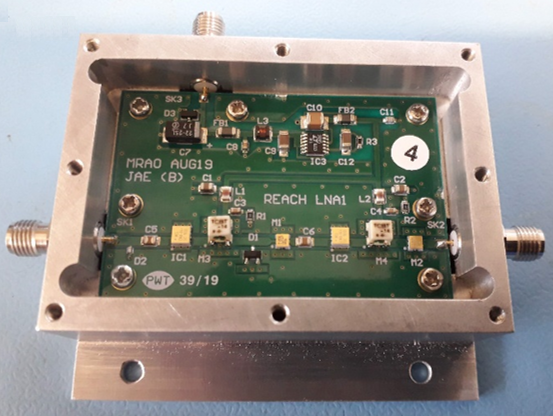
\includegraphics[scale=0.5]{lna}
    \caption{Interior of the completed REACH low noise amplifier custom designed for a flat spectral response in both S\textsubscript{11} and noise.}
    \label{fig:lna}
\end{figure}

While an alternative LNA built instead with Mini-Circuits ERA-50SM+ gain blocks exhibited a better noise figure of 3.3 dB, the CMA-84+ construction demonstrated a better stability in both S\textsubscript{11} and temperature. Reflection coefficients of the finalised LNA are plotted in \cref{fig:lna_sparams} showing the desired S\textsubscript{11} less than -30 dB which is well matched across the observational band as well as a remarkably flat 40 dB gain response.
\begin{figure}
    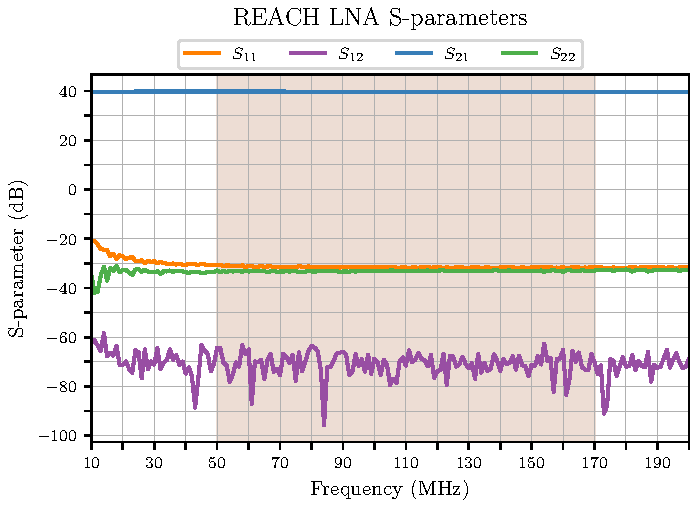
\includegraphics[width=\columnwidth]{lna_sparams}
    \caption{Measured S-parameters of the REACH LNA showing a good match at -30 dB for the $S_{11}$ and $S_{22}$ across the REACH observation band (shaded region) while demonstrating exceptional gain stability ($S_{21}$).}
    \label{fig:lna_sparams}
\end{figure}


% =========================================
\subsubsection{RF signal chain II: Amplifier \#1}
The second stage of spectral data amplification uses another custom module called ‘Amplifier \#1’, or AMP1. Incoming signals from the LNA are further amplified using a Mini-Circuits GALI-S66+ limiting amplifier and a PHA-13LN+ mid-power amplifier in combination to achieve maximal dynamic range followed by high-pass filtering using a Mini-Circuits RHP-44+ filter to attenuate frequencies below the observation band. A 2-stage Mini-Circuits XLF-42M+ monolithic microwave integrated circuit (MMIC) then low-pass filters out-of-band signals above the observation band up to many GHz.

Serving as the internal circuit boundary of the front-end receiver, AMP1 converts signals to Radio-Frequency-over-Fibre for transmission to the receiver back-end minimising the effects of RFI and signal loss that would be typical of alternative connections such as coaxial cables. The passive 1310 nm RFoF converter was made under commission by Polycom according to the specifications for the HERA experiment and has an 18 dB loss due the relative intensity noise of the optical transmission laser which is addressed by 70 dB of upfront gain to reduce the impact of higher noise on the system. The optical transmitter subassembly (as well as the corresponding back-end optical receiver) are printed circuit boards terminated in Fibre Channel/Angled Physical Contact (FC/APC) connectors at the end of a 0.5 metre pigtail as seen in \cref{fig:amp1}.
\begin{figure}
    \centering
    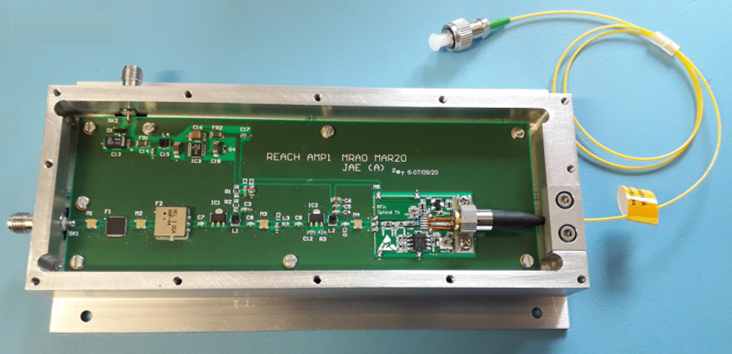
\includegraphics[scale=0.5]{amp1}
    \caption{The REACH AMP1 module used for further amplification and filtering of signals. Seen on the right end of the construction is the fibre optic conversion printed circuit board connected to the single-mode FC/APC RFoF transmission connector seen in yellow.}
    \label{fig:amp1}
\end{figure}
The FC/APC connector links to the RFoF port installed on the front-end enclosure as labelled in \cref{fig:enclosure_external_connections} which connects to an extended roll of fibre optical cabling reaching the receiver back-end. Single-mode fibre optics are again used to prevent signal degradation as with the USB-over-fibre connection. We find the radio-frequency loss of the RFoF bridge over the 100 metre distance to be less than 1 dB including the connections at both ends. A full circuit diagram of amplifier \#1 including the RFoF transducer is shown in \cref{fig:amp1_schematic}.


% =========================================
\subsubsection{Completed receiver front-end unit}
The deployable receiver front-end unit was completed in December 2022 and is shown in \cref{fig:frontend_complete}. 
\begin{figure}
    \centering
    \centering
    \begin{subfigure}{.45\textwidth}
        \centering
        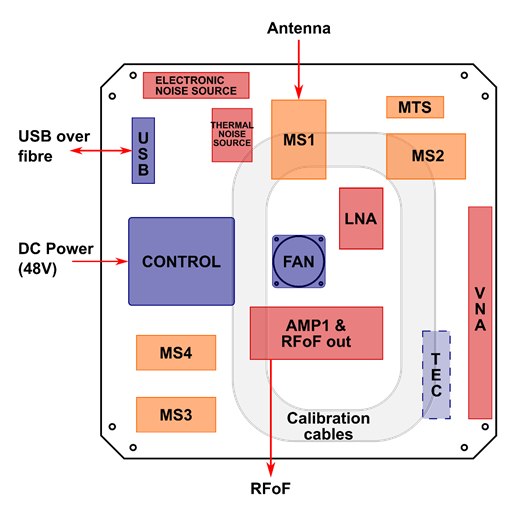
\includegraphics[width=\linewidth]{frontend_layout}
    \end{subfigure}
    \hfill
    \begin{subfigure}{.45\textwidth}
    \centering
        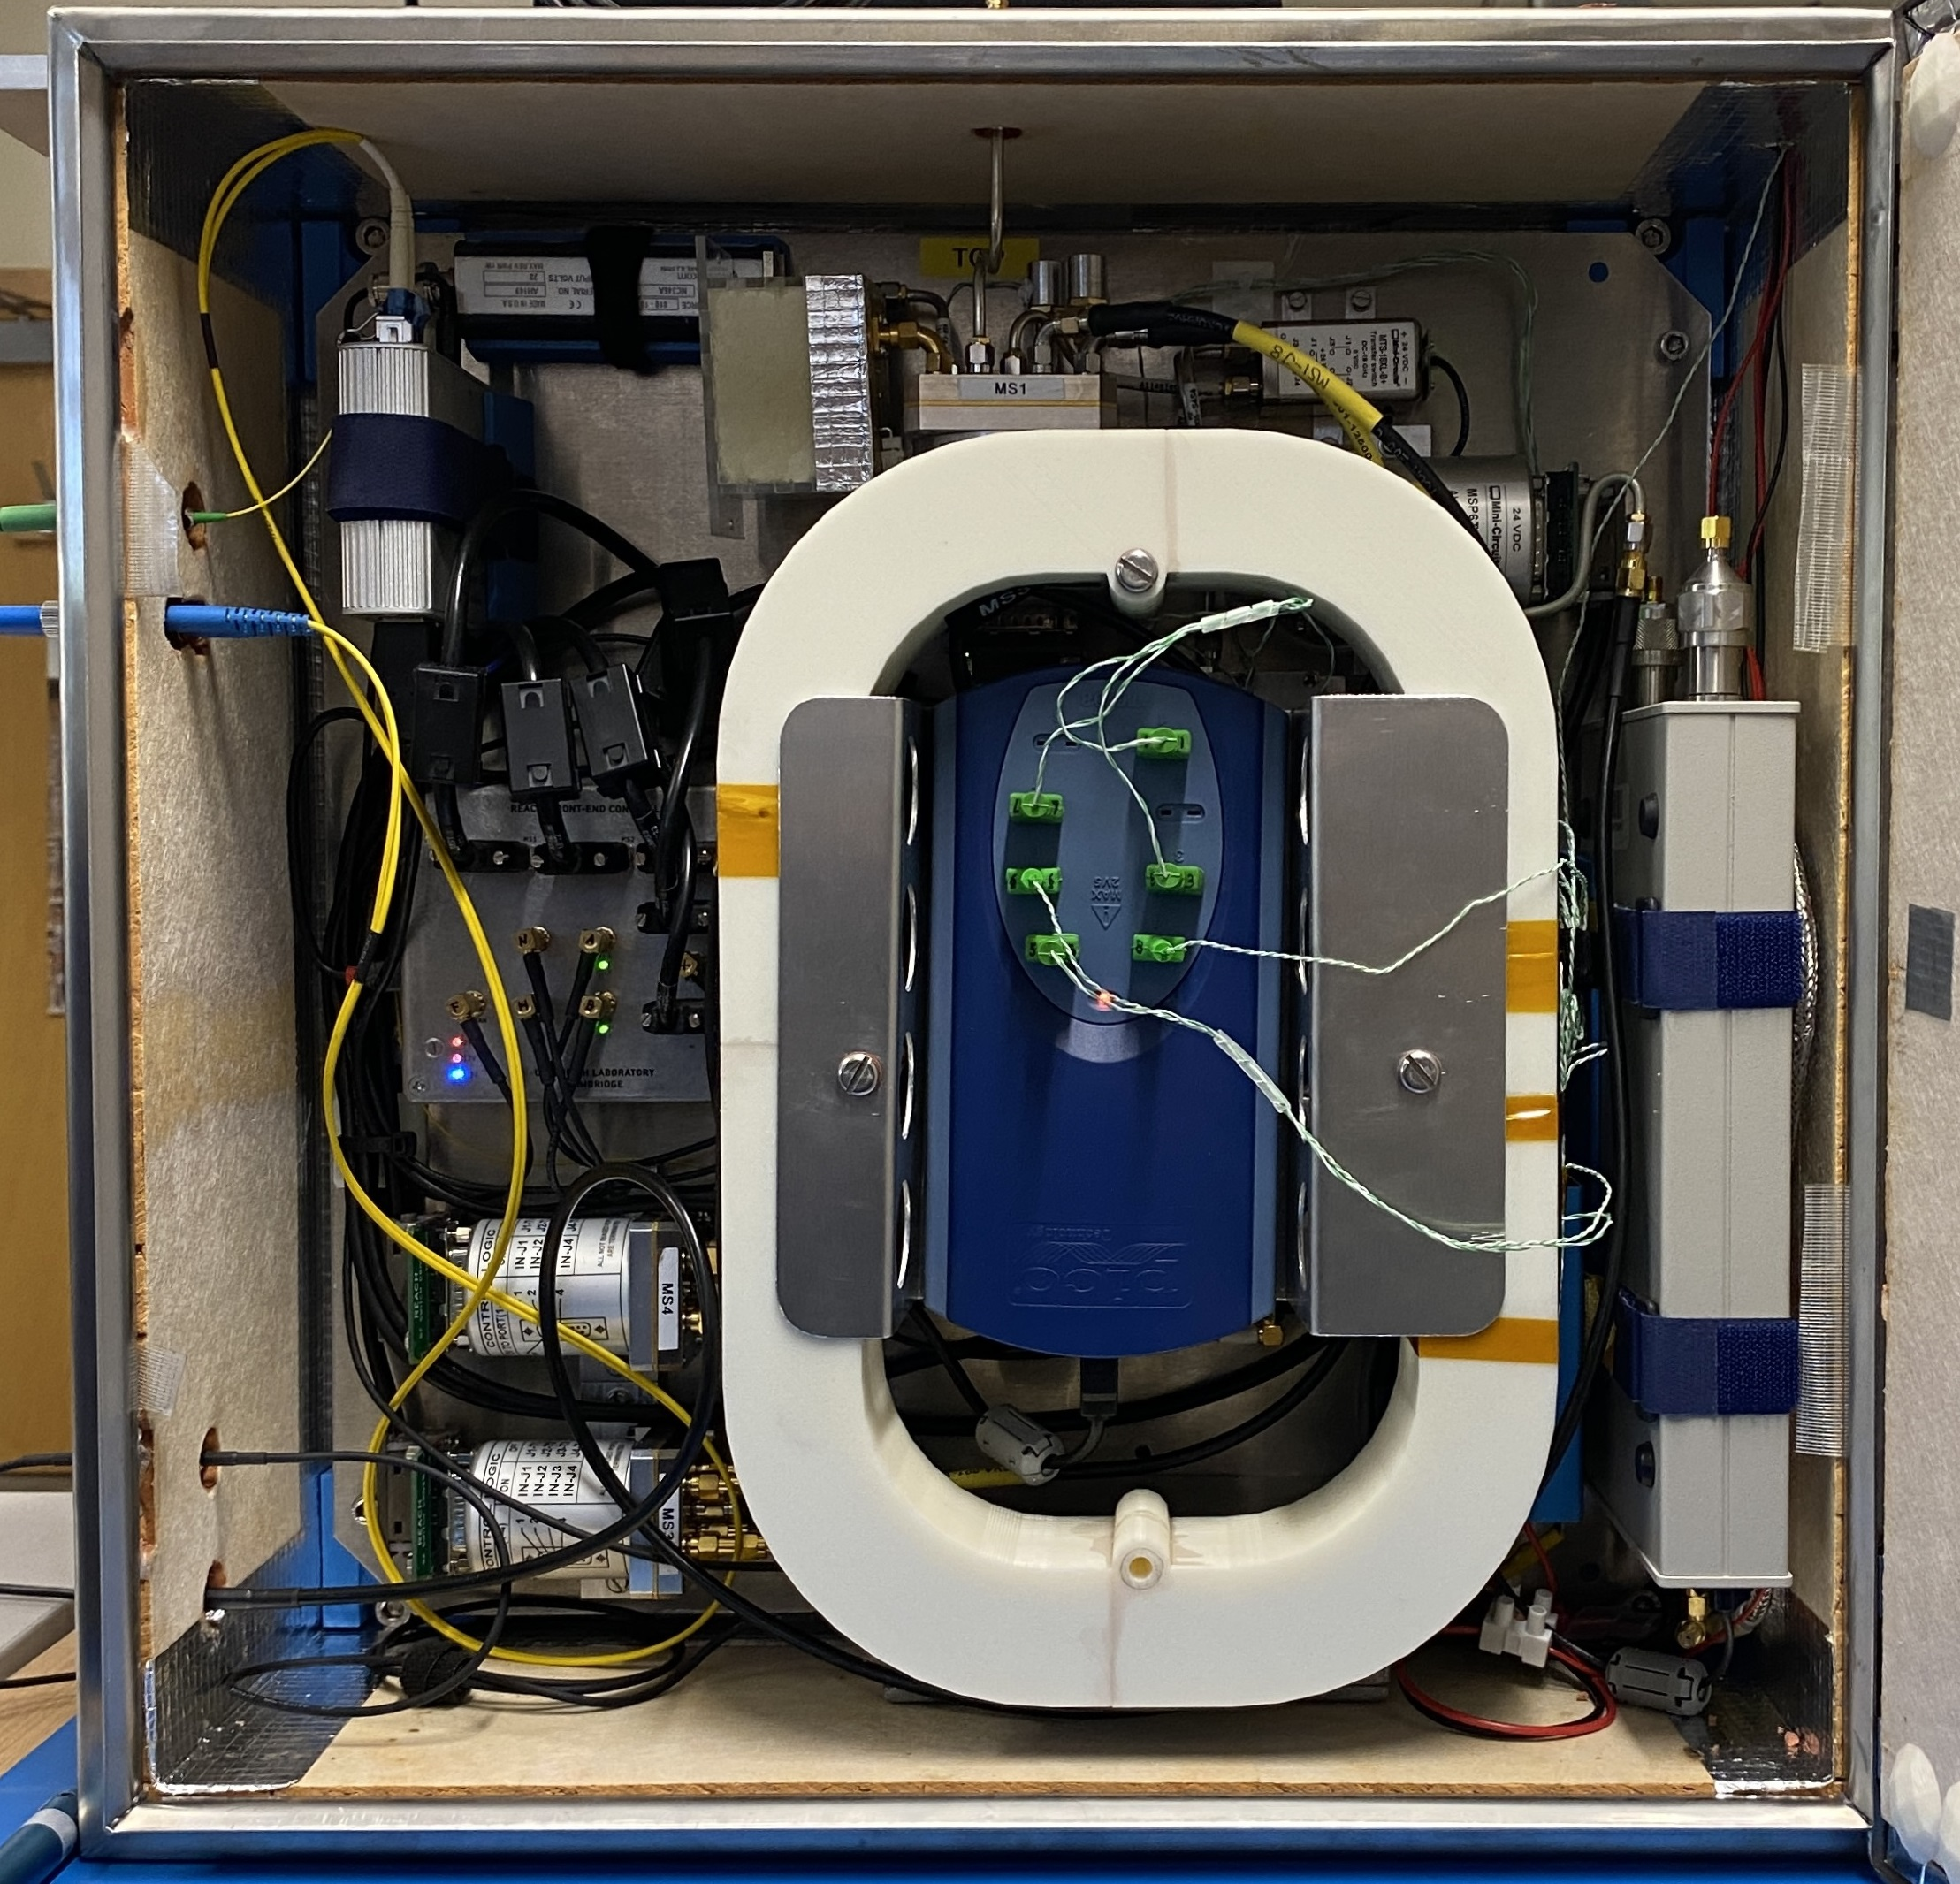
\includegraphics[width=\linewidth]{frontend.jpeg}
    \end{subfigure}
    \caption{The completed receiver front-end unit (right) along with a layout diagram showing the approximate positions of various components (left). Shown in the image are the compact VNA on the bottom right and the TC-08 module in the centre with green thermocouple probes. The stadium housing the calibration cables is seen around the TC-08 and obscures the amplifiers and TEC. The various cylinders are the multi-input switches connected to calibration sources. The microcontroller unit can be seen on the middle-left and is powered on as shown by the LED's. The USB over fibre link and diode noise source are shown in the top left corner.}
    \label{fig:frontend_complete}
\end{figure}
The finalised construction weighs 29 kilograms and, as stated previously, is allocated a maximum of 135 W for total front-end power from the solar panels. Control and RF circuitry require about 31.5 W with the remaining 103.5 W left for cooling through the TEC. The majority of the engineering work went in to construction of this receiver front-end and is expected to be deployed as a portable, energy efficient system with accurate in situ calibration through internal environmental control while maintaining the highest quality measurement capabilities and RFI mitigation. Also included are various ferrite beads to limit control and power signals from intercepting the RF singal path and were generally placed through trial-and-error. Subcomponents along the signal chain are connected with RG-402 semi-rigid cables to prevent cable flexing during transportation. A second 1:1 replica of the receiver is currently being built in Cambridge to assist in remote triage expected during deployment and design changes are being considered for future front-ends to accommodate additional antennas. A picture of the receiver front-end deployed on the REACH site in South Africa is shown in \cref{fig:frontend_deployed}.
\begin{figure}
    \centering
    \includegraphics[scale=0.5]{example-image-c}
    \caption{The receiver front-end in its natural environment, deployed at the REACH experiment site in the Karoo Radio Astronomy Reserve, South Africa.}
    \label{fig:frontend_deployed}
\end{figure}


% =========================================
\subsection{Receiver back-end}
The receiver back-end houses the components critical for remote communication away from the deployment site, power distribution to the instrument as a whole and measurement subsystems that are less sensitive to environmental effects. 100 metres away from the dipole antenna, the receiver back-end sits below ten MODEL NUMBERS solar panels rated to give SPECIFICATIONS HERE as diagrammed in \cref{fig:system_diagram}. This distance was chosen to avoid radio-frequency reflections off the solar panel and back-end faces as well as serving as a potential central node to be equidistant from future antennas. Under the solar panel construction is a radio-frequency electromagnetic-compatibility (RF-EMC) enclosure custom made by Interference Testing and Consultancy Services Ltd. to mitigate the effects of external RFI on our measurements as well as any potential EMI leakage from our own instrument that may be picked up by nearby experiments. Designs for the RF-EMC enclosure were informed by similar constructions used with the HERA experiment that incorporate considerations of the on-site environment as well as compliance with the EMC requirements of the Karoo Radio Astronomy Reserve. A conceptual diagram of the RF-EMC enclosure is shown in \cref{fig:backend}.
\begin{figure}
    \centering
    \centering
    \begin{subfigure}{.45\textwidth}
        \centering
        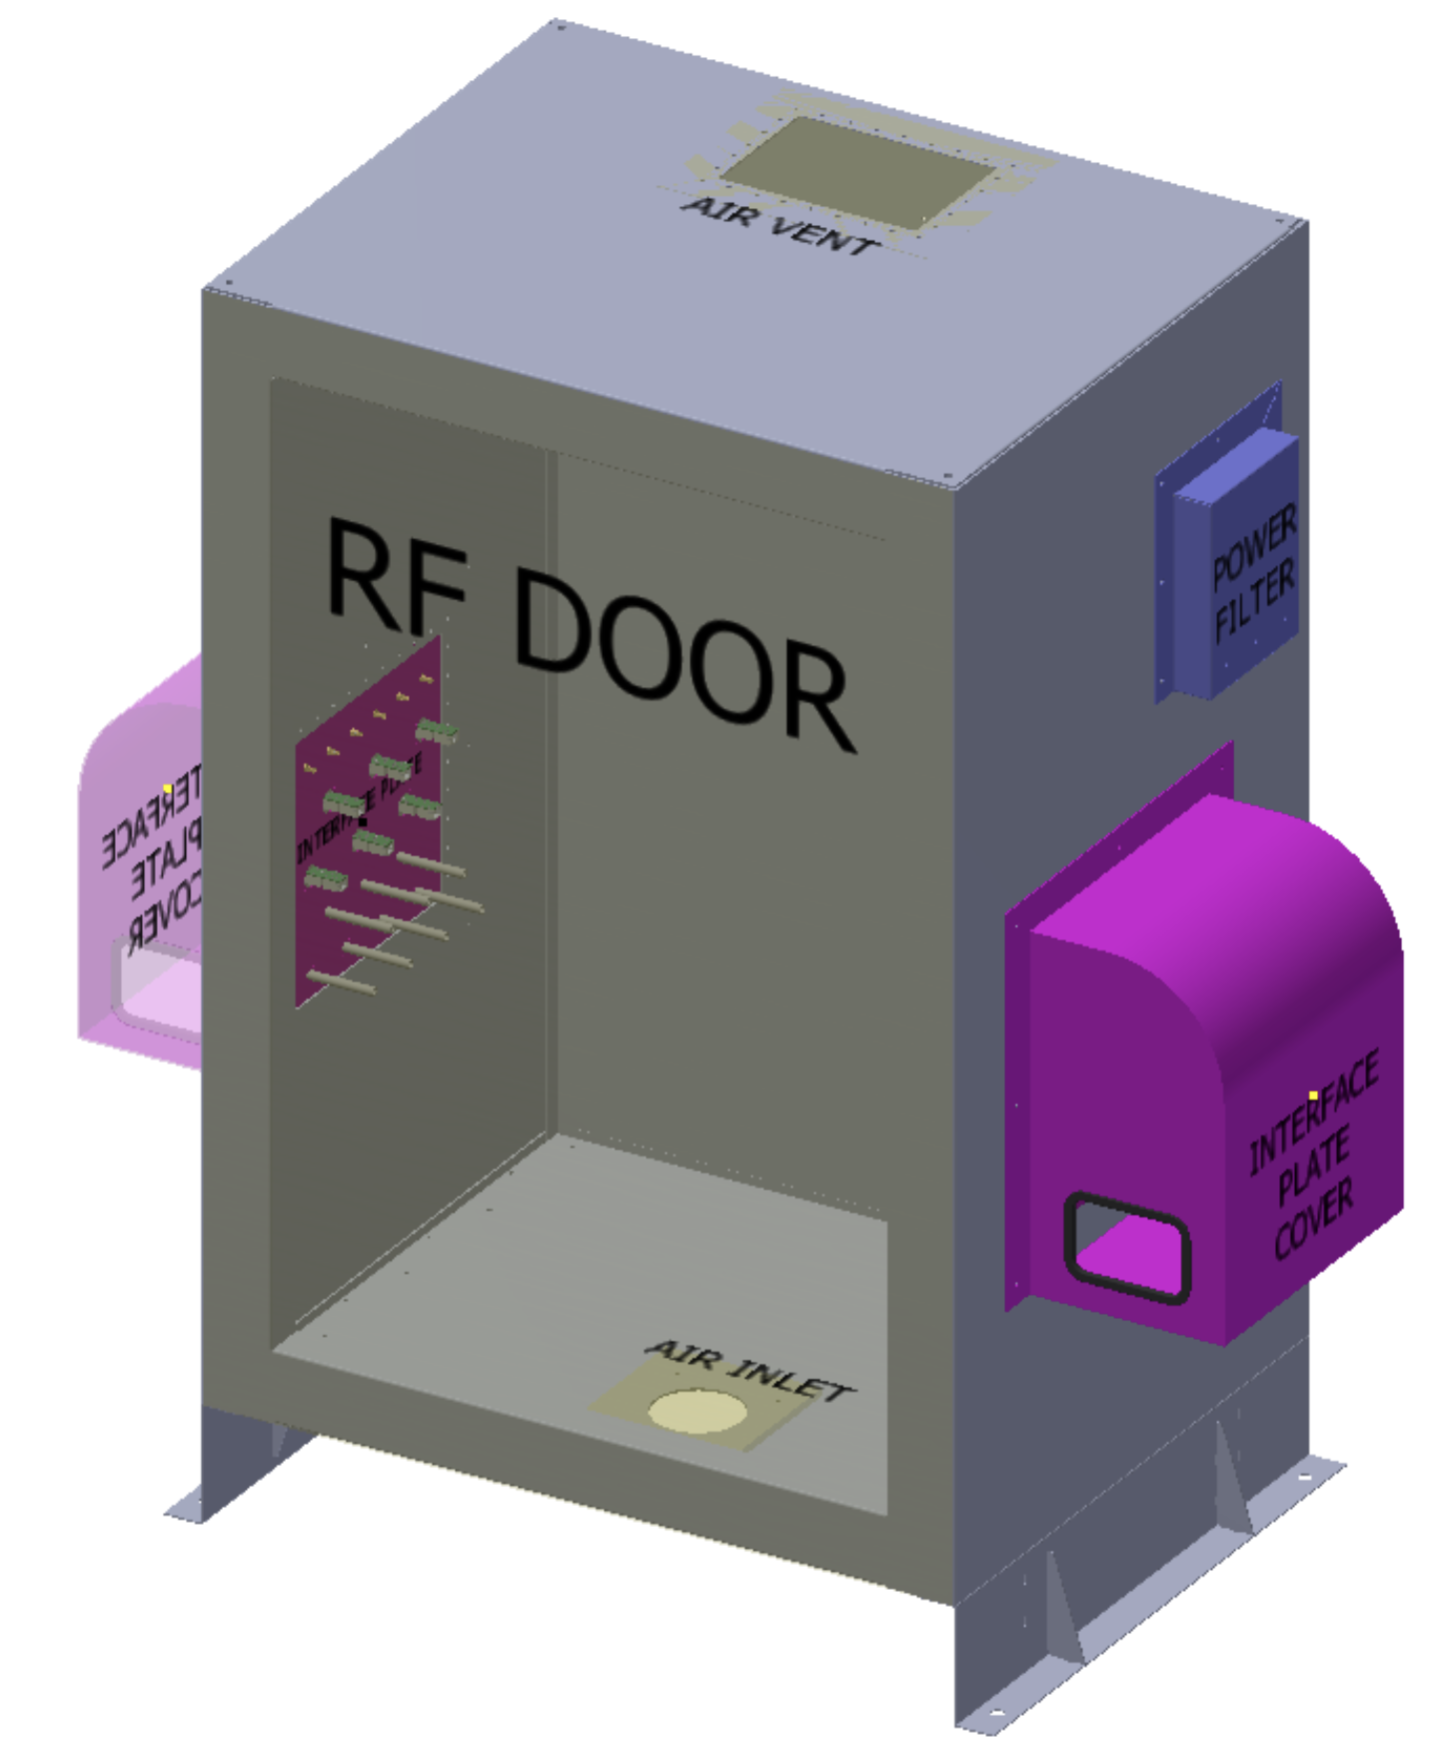
\includegraphics[width=\linewidth]{backend_diag}
    \end{subfigure}
    \hfill
    \begin{subfigure}{.4\textwidth}
    \centering
        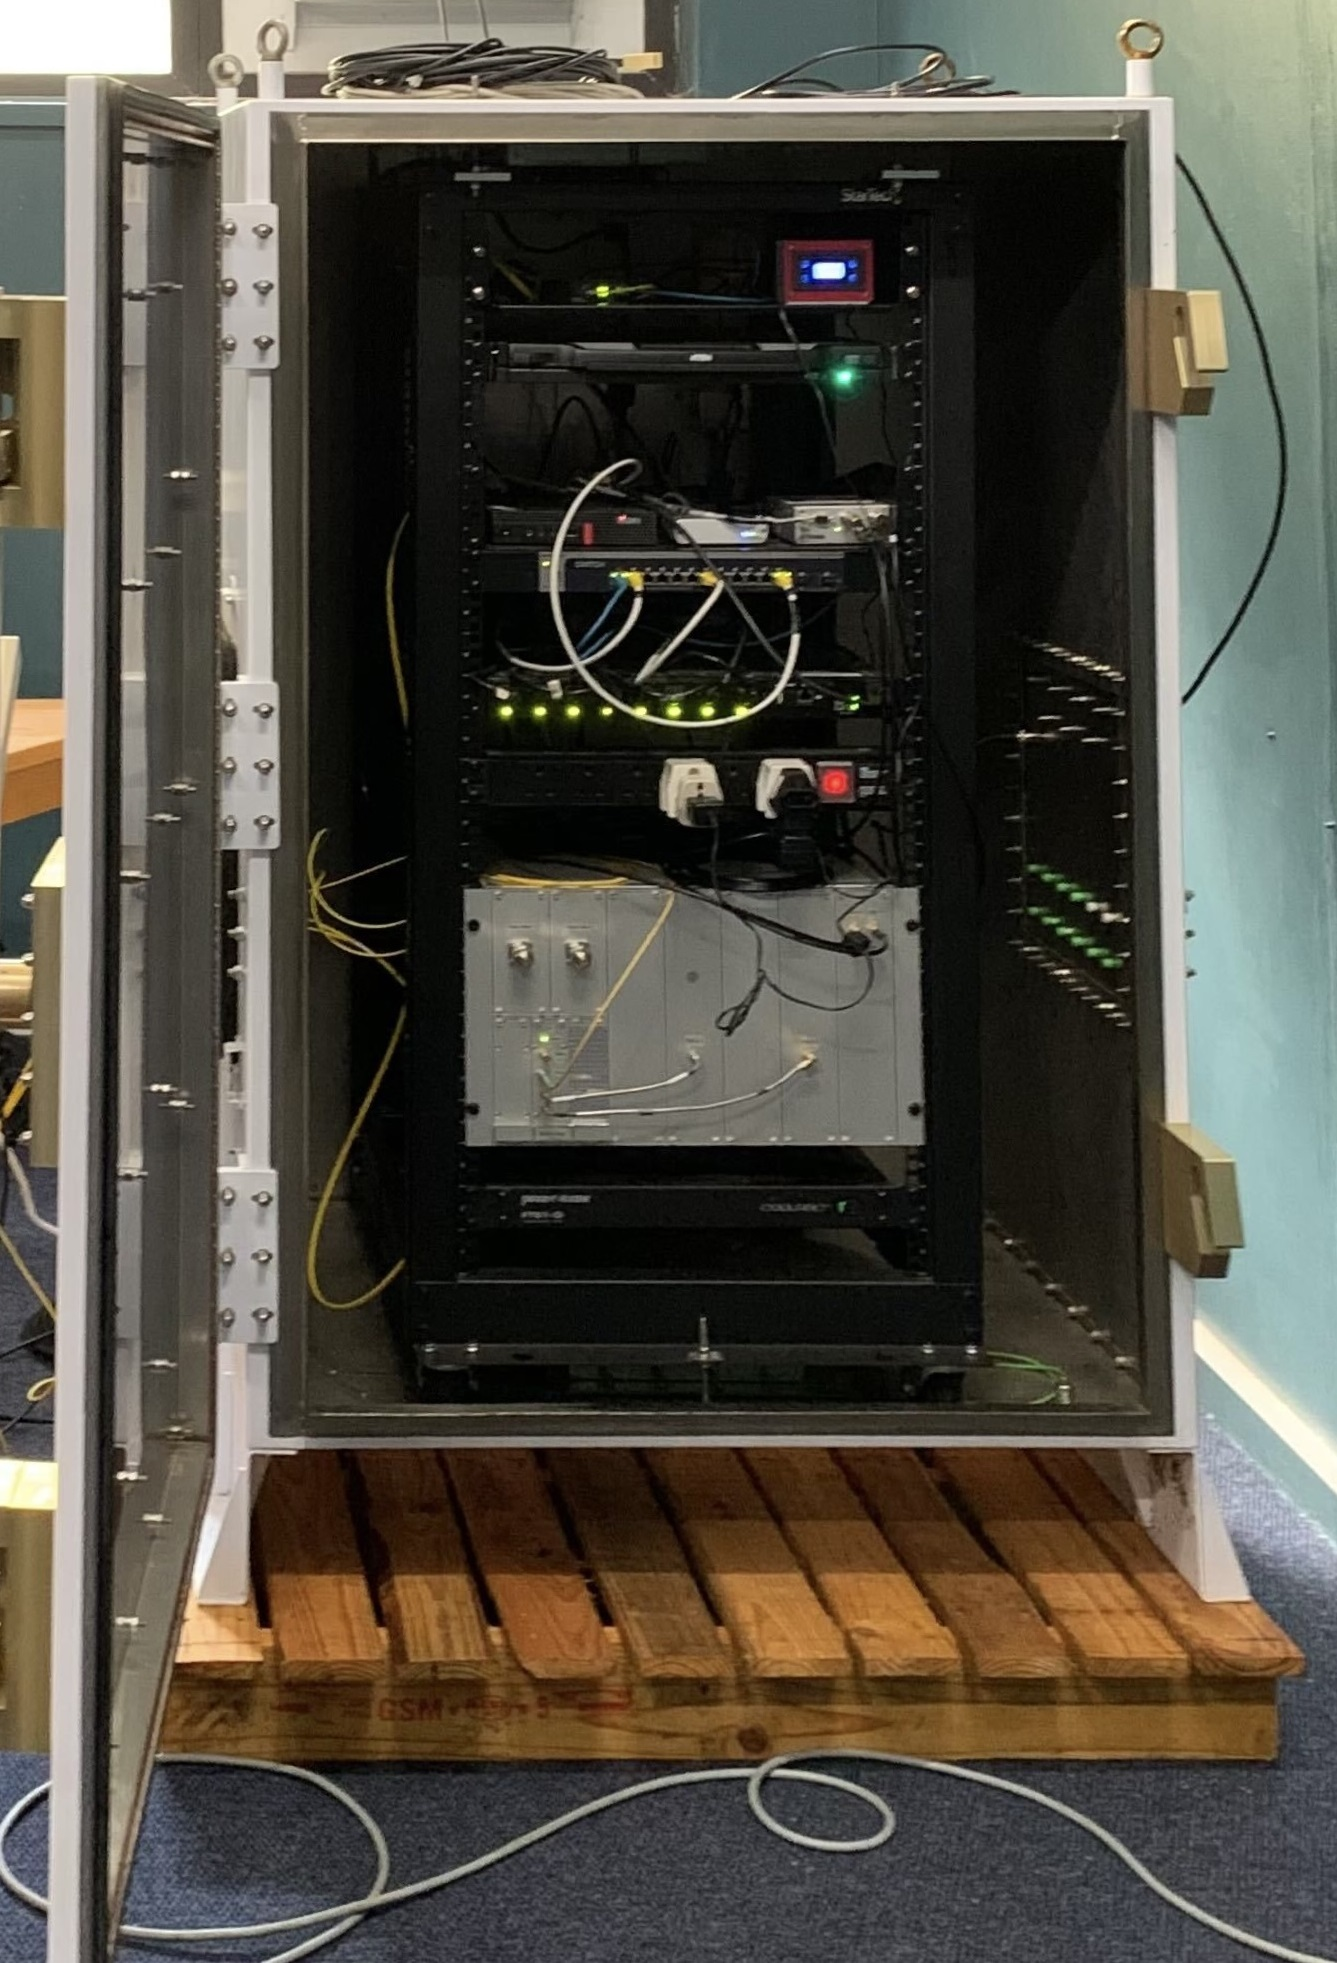
\includegraphics[width=\linewidth]{backend}
    \end{subfigure}
    \caption{A conceptual CAD rendering used as a reference for the REACH back-end RF-EMC enclosure is shown on the left exhibiting various custom assemblies for use in the South African Karoo such as ventilation paths and interference mitigation. The right image shows the completed receiver back-end rack housed inside the RF-EMC enclosure. Rack components such as the amplifier and spectrometer assembly (large silver module), ventilation and power distribution units can be seen.}
    \label{fig:backend}
\end{figure}

Within the RF-EMC enclosure are the various back-end modules mounted on a 36-inch rack\footnote{A StarTech 22U 36in Depth Enclosed Server Cabinet was used in Cambridge but not shipped for deployment.} also shown in \cref{fig:backend} which includes modules for additional signal amplification, conditioning and digitisation, the spectrometer for measurement of power spectral data, the back-end server and GPS system for remote communication and automation of the device, as well as power distribution and cooling units as detailed in this section. The back-end RF-EMC enclosure is accompanied by a smaller similar chamber to house various additional units such as a 7400 Wh SS202 Lithium Iron Phosphate battery made by Solar MD for overnight power storage from the solar panels or during periods of non-ideal weather. This smaller chamber is shown in \cref{fig:power_chamber} for reference but is not strictly a part of the receiver back-end.


% =========================================
\subsubsection{RF signal chain III: Amplifier \#2 and out-of-band injection}


% =========================================
\subsubsection{RF signal chain IV: Simulations}


% =========================================
\subsection{Automation}
\begin{figure}
    \centering
    \includegraphics{controller_pinout}
    \caption{A reference sheet listing the front-end component assignments to the Teensy input/output ports for use in receiver automation. Individual switch positions, power supplies and components can be seen facilitating the creation of new automated routines and on-the-fly system interaction via command line interface. MS‘N’--‘P’ refers to mechanical RF switch number N, port P. MTS is the mechanical transfer switch. TEC is the thermo-electric cooler module.}
    \label{fig:enter-label}
\end{figure}
%\include{Chapter4/chapter4}
%\include{Chapter5/chapter5}
%\include{Chapter6/chapter6}
%\include{Chapter7/chapter7}



% ********************************** Back Matter *******************************
% Backmatter should be commented out, if you are using appendices after References
%\backmatter

% ********************************** Bibliography ******************************
\begin{spacing}{0.9}

% To use the conventional natbib style referencing
% Bibliography style previews: http://nodonn.tipido.net/bibstyle.php
% Reference styles: http://sites.stat.psu.edu/~surajit/present/bib.htm

\bibliographystyle{apalike}
%\bibliographystyle{unsrt} % Use for unsorted references  
%\bibliographystyle{plainnat} % use this to have URLs listed in References
\cleardoublepage
\bibliography{References/references} % Path to your References.bib file


% If you would like to use BibLaTeX for your references, pass `custombib' as
% an option in the document class. The location of 'reference.bib' should be
% specified in the preamble.tex file in the custombib section.
% Comment out the lines related to natbib above and uncomment the following line.

%\printbibliography[heading=bibintoc, title={References}]


\end{spacing}

% ********************************** Appendices ********************************

\begin{appendices} % Using appendices environment for more functunality

% Appendicies =======================================
\ifpdf
    \graphicspath{{Appendix1/Figs/Raster/}{Appendix1/Figs/PDF/}{Appendix1/Figs/}}
\else
    \graphicspath{{Appendix1/Figs/Vector/}{Appendix1/Figs/}}
\fi

\chapter{Supplementary Data} 
\section*{Instrumentation}
\begin{figure}
    \begin{subfigure}{0.49\textwidth}
        \includegraphics[width=\textwidth]{enclosure_back}
    \end{subfigure}
    \hspace*{\fill}
    \begin{subfigure}{0.49\textwidth}
        \includegraphics[width=\textwidth]{enclosure_cross_section}
    \end{subfigure}
    \caption{The completed front-end thermal enclosure is shown on the left. A 3D-rendered cross section in a similar orientation is shown on the right depicting the internal fan, baseplate, Peltier module and heat sink configuration.}
    \label{fig:enclose_supp}
\end{figure}


\begin{table}
    \begin{center}
    \begin{tabular}{ |c|c|c| }
    \hline
    Switch name & Model (Mini-Circuits) & Connection \\
    \hline
    MS1 & 12V MSP8TA-12-12D+ & Calibration sources \\
    MS2 & 24V MSP6TA-12D+& VNA path/calibration components \\
    MS3 & UNKNOWN & 2 metre cable terminations \\
    MS4 & UNKNOWN & 10 metre cable terminations \\
    MTS & 24V MTS-18XL-B+ & Spectrometer/VNA signal path \\
    \hline
    \end{tabular}
    \caption{Switch model number and connections from within the receiver front-end for reference.}
    \label{tab:switches}
    \end{center}
\end{table}

\begin{table}
    \begin{center}
    \begin{tabular}{ |c|c|c| }
        \hline
        {Switch} & {Position} & {Contents}\\
        \hline
        MS1 & 1 & Antenna \\
        MS1 & 2 & Heated $50 \Omega$ load \\
        MS1 & 3 & Reference noise source (diode) \\
        MS1 & 4 & Ambient $50 \Omega$ (cold) load \\
        MS1 & 5 & Ambient $25 \Omega$ load \\
        MS1 & 6 & Ambient $100 \Omega$ load \\
        MS1 & 7 & 2 metre calibration cable \\
        MS1 & 8 & 10 metre calibration cable \\
        \hline
        MS2 & 1 & MTS position 1 (towards calibration sources) \\
        MS2 & 2 & MTS position 3 (towards spectrometer path) \\
        MS2 & 3 & VNA calibration short \\
        MS2 & 4 & VNA calibration open \\
        MS2 & 5 & VNA calibration $50 \Omega$ load \\
        MS2 & 6 & VNA verification $50 \Omega$ test load \\
        \hline
        MS3 & 1 & $36 \Omega$ load \\
        MS3 & 2 & $27 \Omega$ load \\
        MS3 & 3 & $69 \Omega$ load \\
        MS3 & 4 & $91 \Omega$ load \\
        \hline
        MS4 & 1 & Open termination \\
        MS4 & 2 & Shorted termination \\
        MS4 & 3 & $10 \Omega$ load \\
        MS4 & 4 & $250 \Omega$ load \\
        \hline
        MTS & 1 & MS2 position 1 (calibration sources to VNA) \\
        MTS & 2 & MS1 (towards calibration sources) \\
        MTS & 3 & MS2 position 2 (LNA to VNA) \\
        MTS & 4 & Towards LNA (sources to spectrometer)\\
        \hline
    \end{tabular}
    \end{center}
    \caption{The content of each switch position for easy reference. This chart represents the receiver component positions at the time of the December 2022 deployment.}
    \label{tab:switch_content}
\end{table}

\begin{table}
    \centering
    \begin{tabular}{ |c|c|c| }
        \hline
        Power supply & Switchable & Component \\
        \hline
        3.3 V & No & Teensy 3.5 Development Board \\
        5 V & No & Fibre to USB converter \\
        6 V (A) & Yes & Low noise amplifier \\
        6 V (B) & Yes & Low noise amplifier \\
        12 V & Yes & VNA, RF switches \\
        24 V & Yes & Internal fan, RF switches \\
        28 V & Yes & Noise source diode \\
        \hline
    \end{tabular}
    \caption{Power supply considerations for the front-end receiver managed by the microcontroller unit. The ability to toggle the 5 V supply was disabled at the hardware-level in order to prevent accidental user activation which would result in a (catastrophic) completely non-responsive instrument.}
    \label{tab:power_supply}
\end{table}

\begin{figure}
    \centering
    \includegraphics[angle=90,width=0.95\textwidth]{amp1_schematic}
    \caption{Full circuit diagram for amplifier \#1 in the REACH receiver front-end. Credit: John A. Ely and Nima Razavi-Ghods.}
    \label{fig:amp1_schematic}
\end{figure}

\begin{figure}
    \centering
    \includegraphics[scale=0.2]{power_chamber.jpeg}
    \caption{The smaller RF-EMC chamber accompanying the receiver back-end. This chamber houses various additional units for overnight power storage from the solar panels. The black module adorned with the yellow "X" symbol is the Solar MD SS202 Lithium Iron Phosphate battery.}
    \label{fig:power_chamber}
\end{figure}

\begin{figure}
    \centering
    \includegraphics[angle=90,width=0.95\textwidth]{amp2_schematic}
    \caption{Full circuit diagram for amplifier \#2 in the REACH receiver back-end. Credit: John A. Ely and Nima Razavi-Ghods.}
    \label{fig:amp2_schematic}
\end{figure}

\begin{table}
    \begin{center}
    \begin{tabular}{ |c|c| }
    \hline
    Port Number & Device \\
    \hline
    7--24 V DC GND & Penn Elcom FT01-Q Cooling rack\\
    Port 0 & Lenovo ThinkCentre server \\
    Port 1 & ATEN CL6700 MW KVM module \\
    Port 2 & Netgear ProSafe M4100-D12G Ethernet switch \\
    Port 3 & Icron 2244 USB Ranger \\
    Port 4 & Unused \\
    Port 5 & Unused \\
    Port 6 & Readout system TEC controller USB connection \\
    Port 7 & Unused \\
    Port 8 & Unused \\
    Port 9 & Unused \\
    Port 10 & Unused \\
    \hline
    \end{tabular}
    \caption{Receiver back-end StarTech USB hub connections.}
    \label{tab:usb_hub}
    \end{center}
\end{table}

\begin{table}
    \begin{center}
    \begin{tabular}{ |c|c| }
    \hline
    Port Number & Device \\
    \hline
    Port 1 & Unused \\
    Port 2 & Readout system Ethernet output \\
    Port 3 & Unused \\
    Port 4 & Unused \\
    Port 5 & Unused \\
    Port 6 & Unused \\
    Port 7 & Lenovo ThinkCentre Ethernet input \\
    Port 8 & Unused \\
    Port 9 & Unused \\
    Port 10 & Unused \\
    Port 11 & Unused \\
    Port 12 & Tripp Lite PDUMH15HVNET power distribution unit \\
    \hline
    \end{tabular}
    \caption{Receiver back-end Netgear ProSafe M4100-D12G Ethernet switch connections.}
    \label{tab:eth_switch}
    \end{center}
\end{table}

\begin{table}
    \begin{center}
    \begin{tabular}{ |c|c| }
    \hline
    Port Number & Device \\
    \hline
    Port 1 & Penn Elcom FT01-Q cooling rack\\
    Port 2 & Netgear ProSafe M4100-D12G Ethernet switch (power connection) \\
    Port 3 & Lenovo ThinkCentre \\
    Port 4 & Icron 2244 USB Ranger \\
    Port 5 & Trimble Thunderbolt E GPS disciplined clock\\
    Port 6 & Readout enclosure power \\
    Port 7 & Second back-end power distribution unit \\
    Port 8 & ATEN CL6700 MW KVM module \\
    Ethernet port & Netgear ProSafe M4100-D12G Ethernet switch (Ethernet connection) \\
    \hline
    \end{tabular}
    \caption{Receiver back-end Tripp Lite PDUMH15HVNET power distribution unit connections.}
    \label{tab:backend_pdu}
    \end{center}
\end{table}
%!TEX root = ../thesis.tex
% ******************************* Thesis Appendix B ********************************

\chapter{Installing the CUED class file}

\LaTeX.cls files can be accessed system-wide when they are placed in the
<texmf>/tex/latex directory, where <texmf> is the root directory of the user’s \TeX installation. On systems that have a local texmf tree (<texmflocal>), which
may be named ``texmf-local'' or ``localtexmf'', it may be advisable to install packages in <texmflocal>, rather than <texmf> as the contents of the former, unlike that of the latter, are preserved after the \LaTeX system is reinstalled and/or upgraded.

It is recommended that the user create a subdirectory <texmf>/tex/latex/CUED for all CUED related \LaTeX class and package files. On some \LaTeX systems, the directory look-up tables will need to be refreshed after making additions or deletions to the system files. For \TeX Live systems this is accomplished via executing ``texhash'' as root. MIK\TeX users can run ``initexmf -u'' to accomplish the same thing.

Users not willing or able to install the files system-wide can install them in their personal directories, but will then have to provide the path (full or relative) in addition to the filename when referring to them in \LaTeX.

\end{appendices}

% *************************************** Index ********************************
\printthesisindex % If index is present

\end{document}
